\section{Evaluation Design}
\label{sec:eval}
In this section, we describe a series of experiments, which are specifically designed to study the QoE performance of using QUIC and HTTP/2 for ABR video streaming with a focus on segment retransmission. We compare the results of these experiments  with the baseline approach that uses HTTP/1.1. The server nodes (denoted as \textit{Server1 - Server4} in Fig. \ref{fig:clab_topo}) run a Caddy server (version=0.10.10) \cite{caddy} with the experimental QUIC mode enabled such that the clients can stream DASH videos either over TCP or QUIC. We chose the Caddy server as it is a production server which is capable of simultaneously supporting QUIC, HTTP1.1, and HTTP/2 over TCP with TLS1.2. All experiments use an excerpt of the \texttt{BigBuckBunny} dataset \cite{lederer2012dynamic} (unless stated otherwise) that comprises a 300s-long video with a 2s segment duration and the corresponding MPD file. We extended the MPD file by providing the size of each segment in each of the available quality levels.\footnote{We use segment sizes in the MPD file since this was introduced in AStreamer. This can easily be replaced by using byte ranges, which are available in real-world, ABR streaming solutions.} The quality bitrates available in this MPD file are the following: $\{${0.09, 0.13, 0.18, 0.22, 0.26, 0.33, 0.59, 0.79, 1.03, 1.24, 1.54, 2.48, 3.52, 4.21}$\}$Mbps. The client nodes run the SQUAD ABR algorithm~\cite{Wang:TOMM:2017} described above, which is implemented in a Python-based DASH player~\cite{parikshit:icc}.

\begin{figure}
\centering
% \includegraphics[scale=0.40, trim={0mm 120mm 0mm 20mm}]
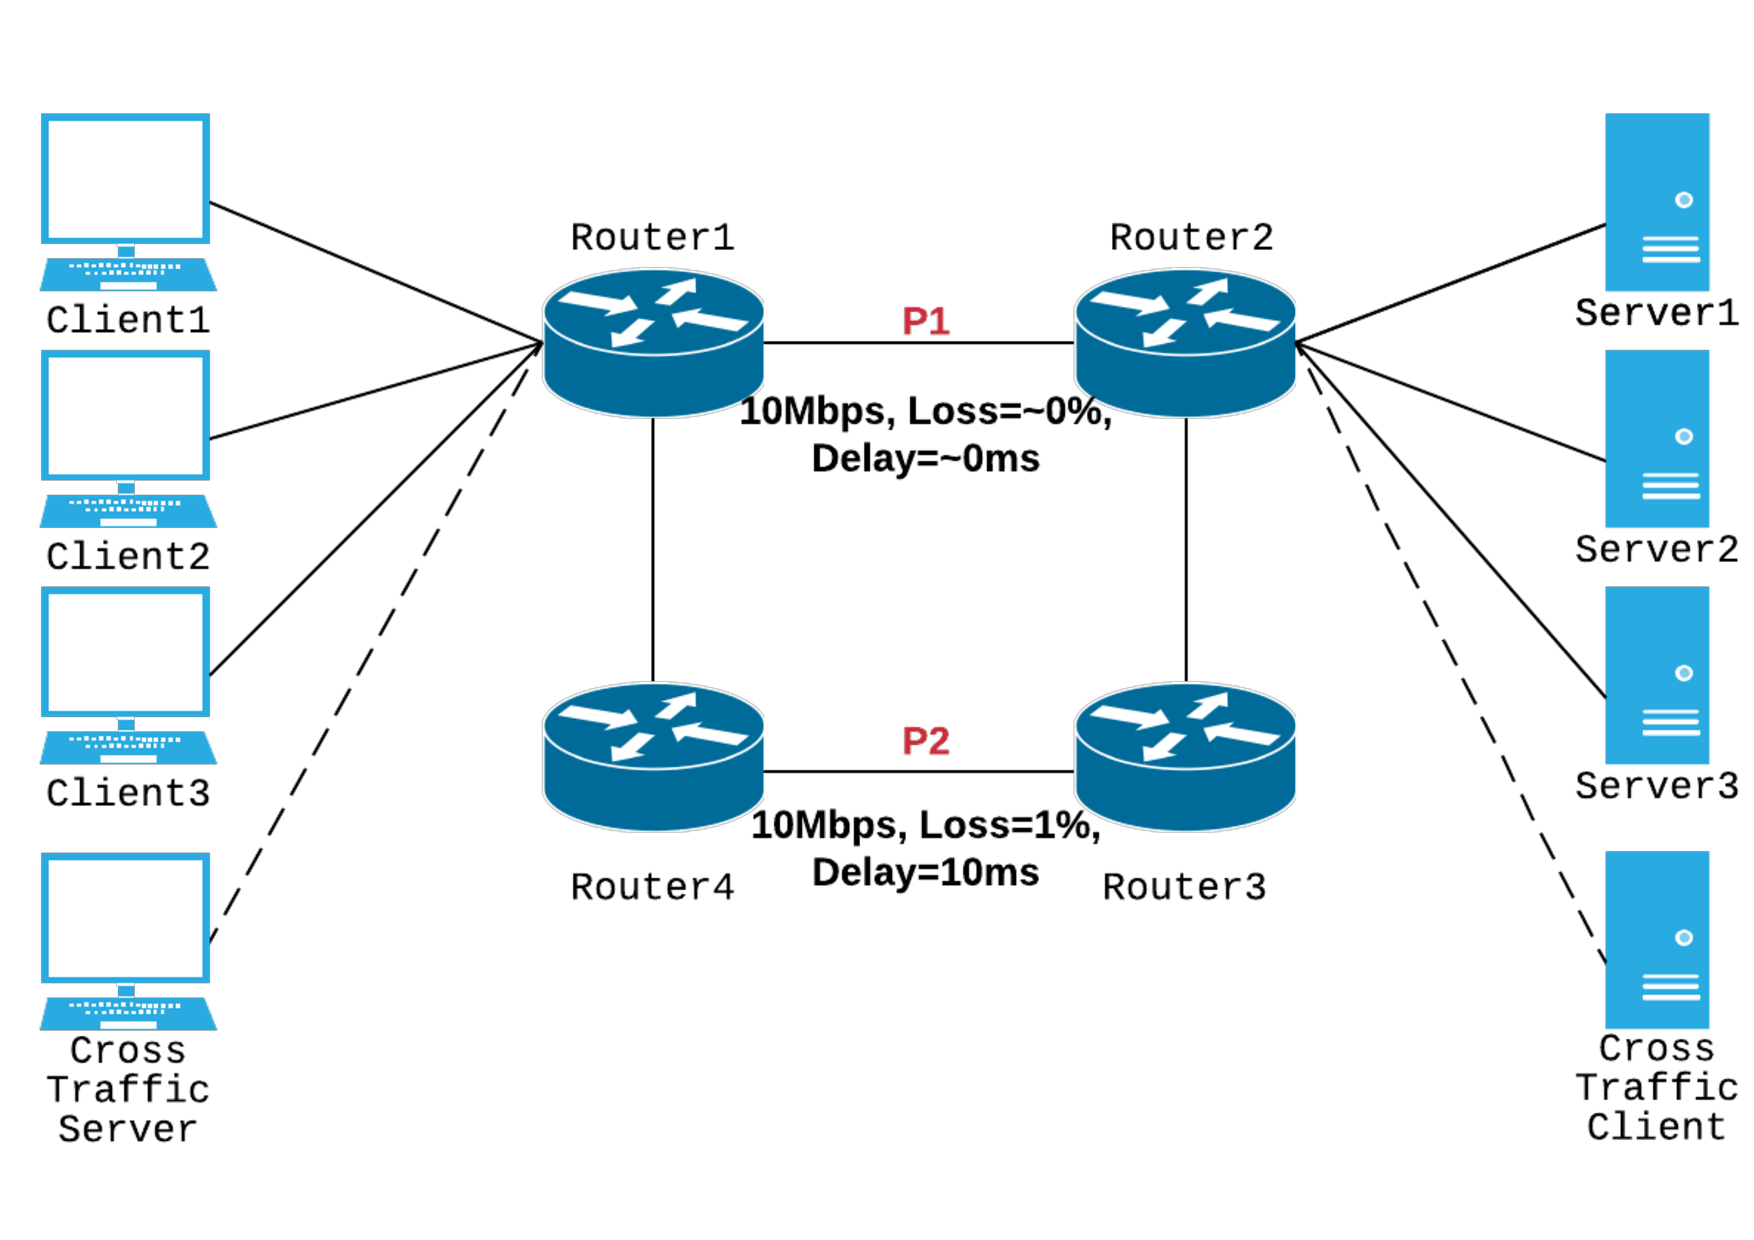
\includegraphics[width=\linewidth,angle=0,scale=0.85, trim={2cm 2cm 2cm 2cm}]{figures/ACM_MM18_topo_v2.pdf}
\caption{Cloudlab topology used for controlled experiments}
\label{fig:clab_topo}
\vspace{-20pt}
\end{figure}

\label{sec:eval}
\begin{comment}
\subsection{Segment Download Time}
As stated in previous work~\cite{Wang:TOMM:2017}{}, the SQUAD algorithm uses the following two equations in order to reliably estimate if the retransmission of a segment can be successfully performed before its playout deadline. 
\DB{Add Eq12 and Eq13 from TOMM paper - should I add these or is it unnecessary?}. Our first set of experiments compares the download times of varying segment sizes, which we believe will lend valuable insight to evaluate the ABR streaming experiments that follow. 
In order to utilize the benefit of the multiplexing feature of HTTP/2 and QUIC for SQUAD, we make slight modifications to the implementation without altering the details of the SQUAD algorithm itself.
\end{comment}
\subsection{Testbed}
For our controlled experiments, we use Cloudlab \cite{RicciEide} which is a geographically distributed testbed for
the development, deployment, and validation of cloud-based services. The CloudLab infrastructure consists of several different racks of varying compute and storage resources designed to provide isolated performance. The topology shown in Fig.~\ref{fig:clab_topo} consists of four clients and four servers connected by two paths \textbf{P1} and \textbf{P2} with the default set to \textbf{P1} unless stated otherwise. All nodes run vanilla Ubuntu 14.04 where all TCP related experiments use TCP Cubic. In order to account for statistical variance, every experiment in the controlled environment is repeated 30 times. For the single client experiments, we use \textit{Client1} and \textit{Server1} as the default pair and include other server and client pairs for parallel client cases.
\begin{figure*}[t!]
\centering
\begin{subfigure}[t]{0.33\textwidth}
   \captionsetup{justification=centering,margin=4.5cm}
    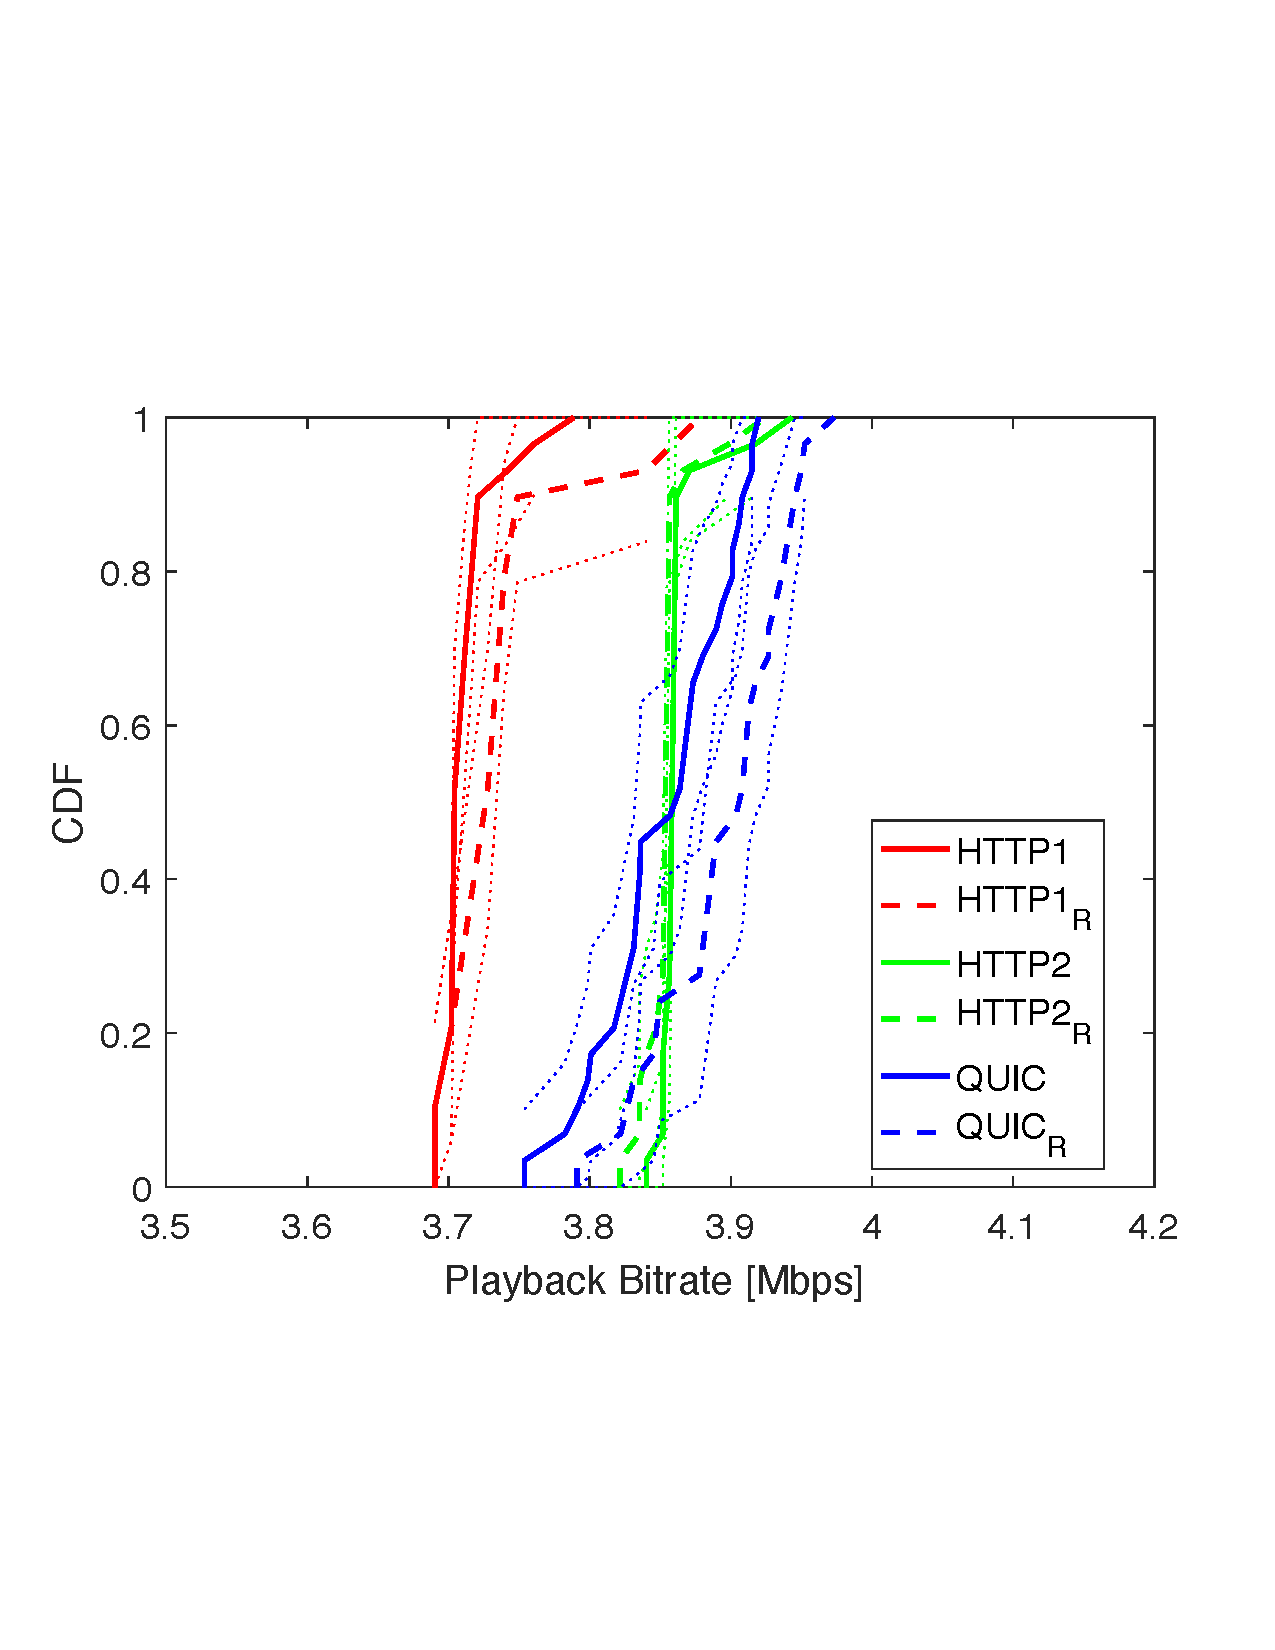
\includegraphics[trim={0 5cm 0 6cm}, scale=0.24]{figures/CDF_bitrat_squad_udpstair_nd18.pdf}
     \caption{}
    \label{fig:udpstairbitrate}
  \end{subfigure}
  \begin{subfigure}[t]{0.33\textwidth}
  \captionsetup{justification=raggedright,singlelinecheck=false,margin=2.5cm}
    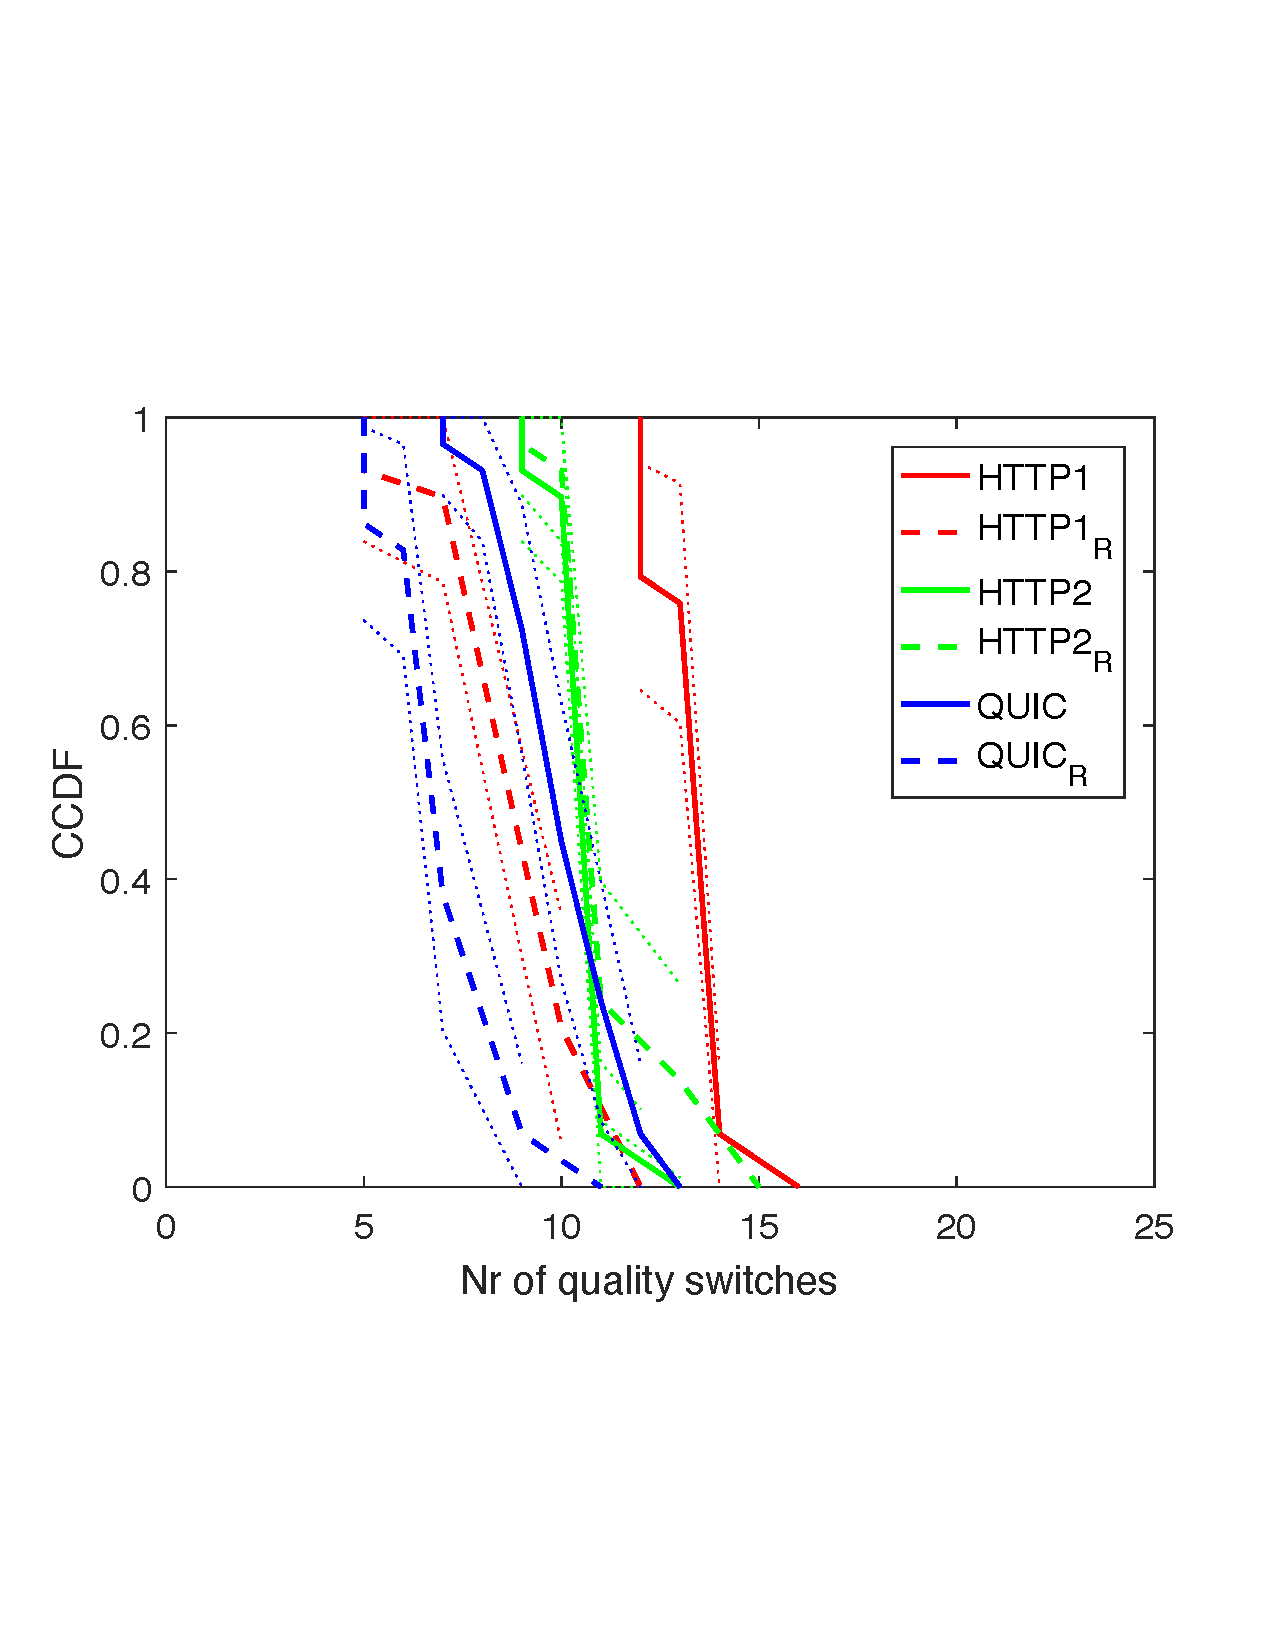
\includegraphics[trim={0 5cm 0 6cm}, scale=0.24]{figures/CDF_cntswitch_squad_udpstair_nd18.pdf}
    \caption{}
    \label{fig:udpstaircntsw}
  \end{subfigure}
  \begin{subfigure}[t]{0.33\textwidth}
  \captionsetup{justification=centering,margin=1.5cm}
    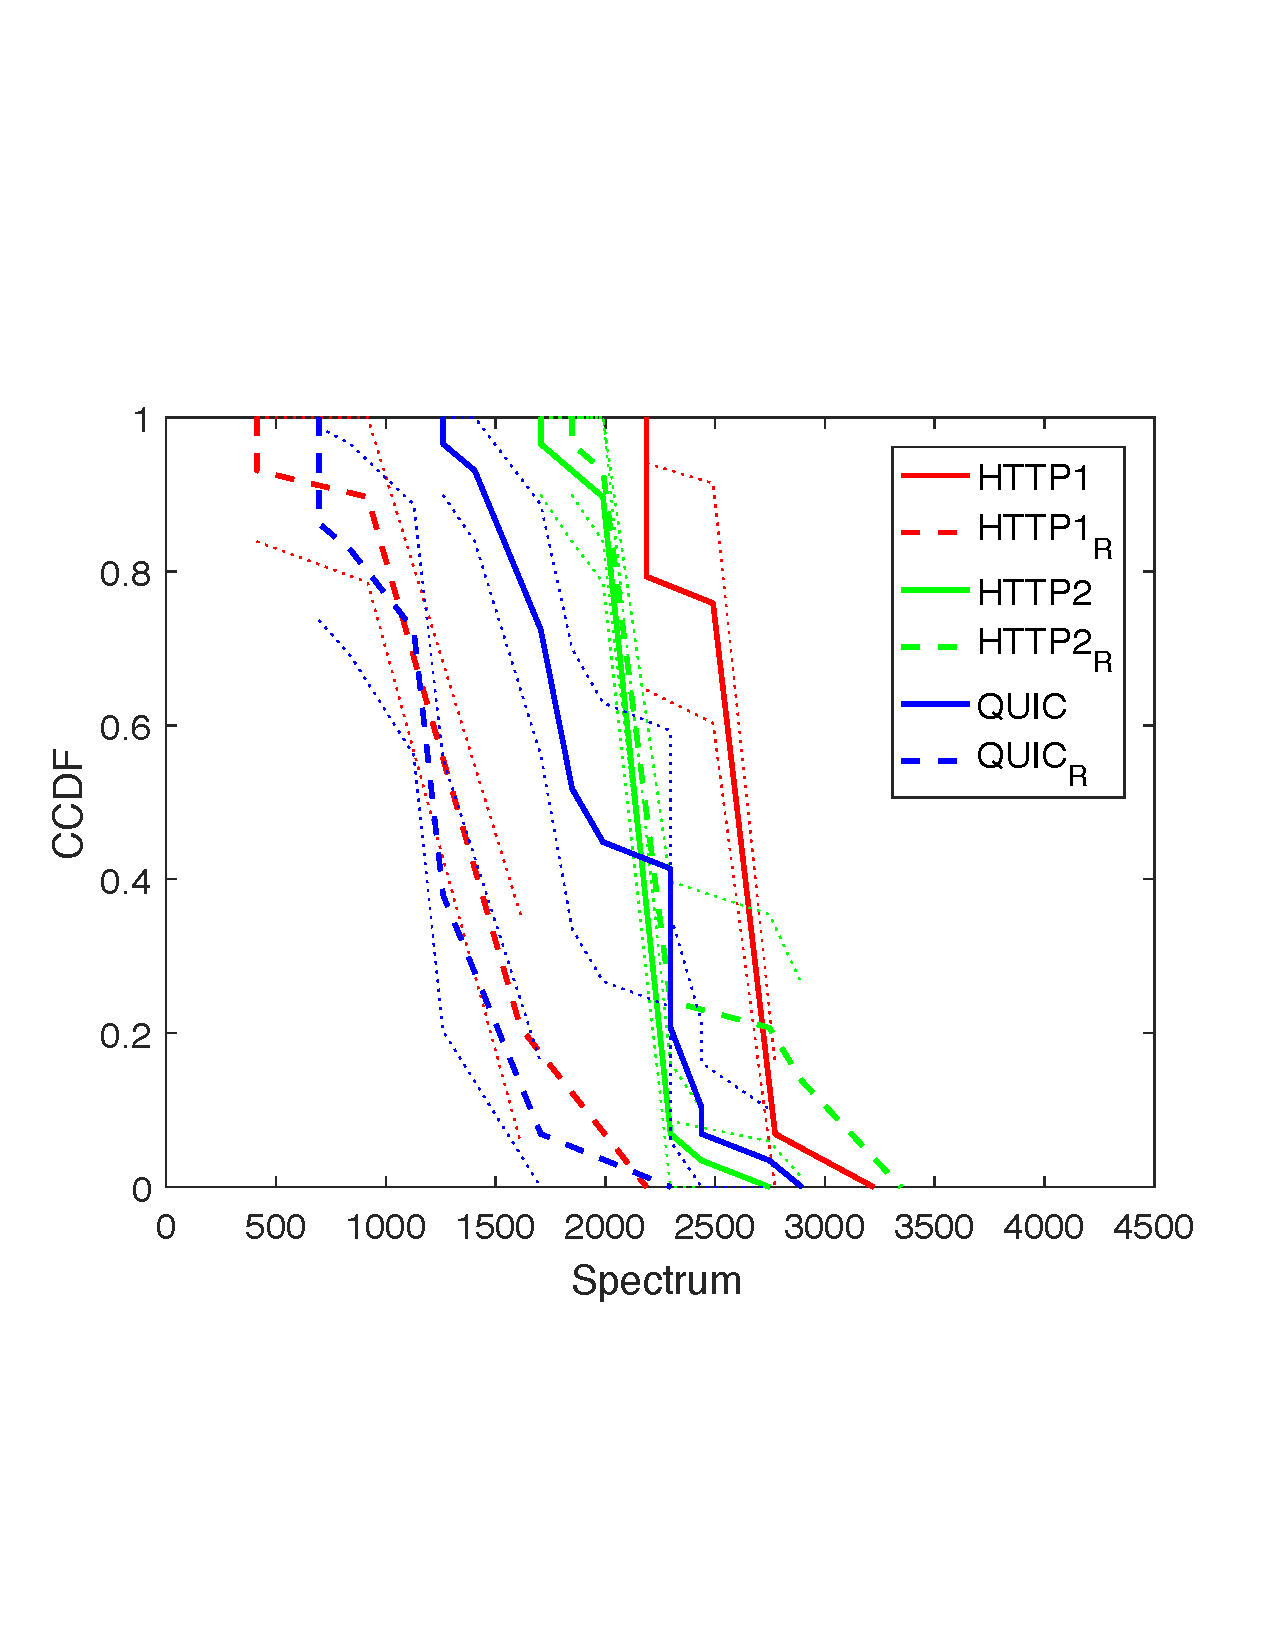
\includegraphics[trim={0 5cm 0 6cm}, scale=0.24]{figures/CDF_magswitch_squad_udpstair_nd18.pdf}
    \caption{}
    \label{fig:udpstairmagsw}
  \end{subfigure}
 \centering
   \vspace{-15pt}
  \caption{Single Client Measurements - Rate Limited with UDP-Staircase cross traffic. 
  %Here, we see results of using a stepwise UDP cross traffic increasing in increments of 3Mbps upto a maximum of 9Mbps where 
  QUIC has a significantly better overall Quality of Experience compared to HTTP/1.1 and HTTP/2, which is further improved by retransmissions. Note, subscript ``R'' denotes ABR segment retransmissions.}
  \label{fig:udpstair}
   \vspace{-10pt}
\end {figure*}
\subsubsection{Single Client: Rate Limiting with UDP}
\label{subsubsec:single_udp}
In order to systematically compare the performance of HTTP/1.1, HTTP/2 and QUIC in a controlled environment, we use the \texttt{Iperf}\footnote{\url{https://iperf.fr/iperf-doc.php}} application to generate competing UDP traffic (denoted cross traffic) of varying amplitudes. The first set of experiments consists of repeating a stepwise variation of cross traffic where the duration of each step is 11s and varies as follows: \{0-11s: 0Mbps, 12-23s: 3Mbps, 24-35s: 6Mbps, 36-55s: 9Mbps, 56-67s: 6Mbps, 68-79s: 3Mbps, 80-91s: 0Mbps\} (then the pattern repeats until t=300s). Fig. \ref{fig:udpstair} shows the CDF and CCDF along with 95\% confidence intervals for upper and lower bounds of the QoE metrics described at the beginning of this section. In Fig. \ref{fig:udpstairbitrate}, we observe that QUIC clients have the highest average quality bitrate or $AQB$ when compared to both HTTP/1.1 and HTTP/2. It is also worth noting that other QoE metrics such as number of quality changes ($\#QS$) and the Spectrum, $H$, are significantly improved with the use of QUIC retransmissions. Figure \ref{fig:udpw9} shows results for the "W" cross traffic case where we use the \texttt{Iperf} application to generate competing UDP cross traffic that creates a "W" shaped bottleneck bandwidth and varies as follows: \{0-20s: 9Mbps, 21-40s: 5Mbps, 41-60s: 9Mbps, 61-80s: 0Mbps\} (then the pattern repeats until t=300s). Although, in terms of $AQB$, $\#QS$ and $H$, HTTP/2 clients appear to experience the best QoE, we observed that the clients also experience a relatively high rebuffering ratio, $RB$, of 4\% while using HTTP/2 for ABR streaming. Since it is well known that the foremost objective of any ABR client streaming algorithm is to eliminate or reduce rebuffering, we conclude that QUIC, especially with the use of segment retransmissions, also performs significantly better than HTTP/1.1 and HTTP/2 for the "W" cross traffic case. 
\begin{figure*}[htb!]
\centering
\begin{subfigure}[t]{0.33\textwidth}
   \captionsetup{justification=centering,margin=4.5cm}
    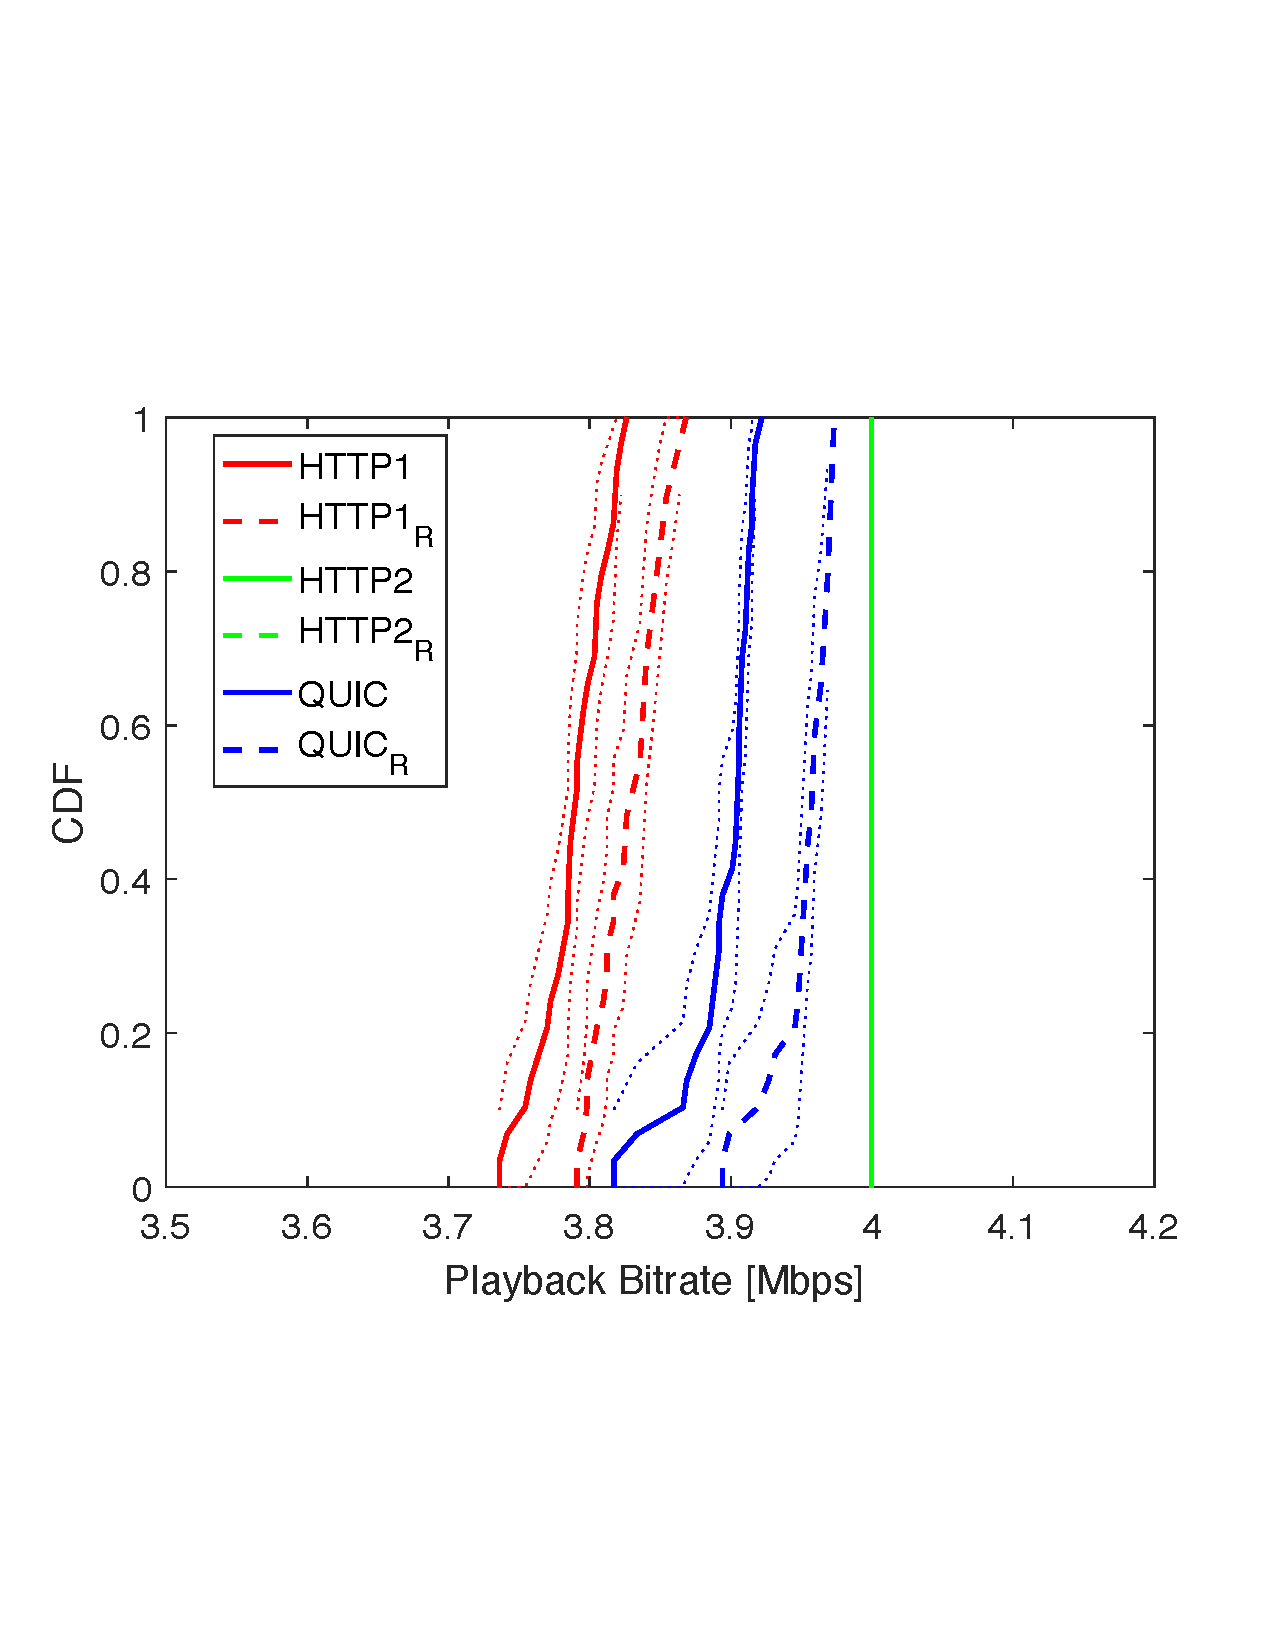
\includegraphics[trim={0 5cm 0 7cm}, scale=0.24]{figures/CDF_bitrat_squad_udpw9_nd18.pdf}
     \caption{}
    \label{fig:udpw9bitrate}
  \end{subfigure}
  \begin{subfigure}[t]{0.33\textwidth}
  \captionsetup{justification=raggedright,singlelinecheck=false,margin=2.5cm}
    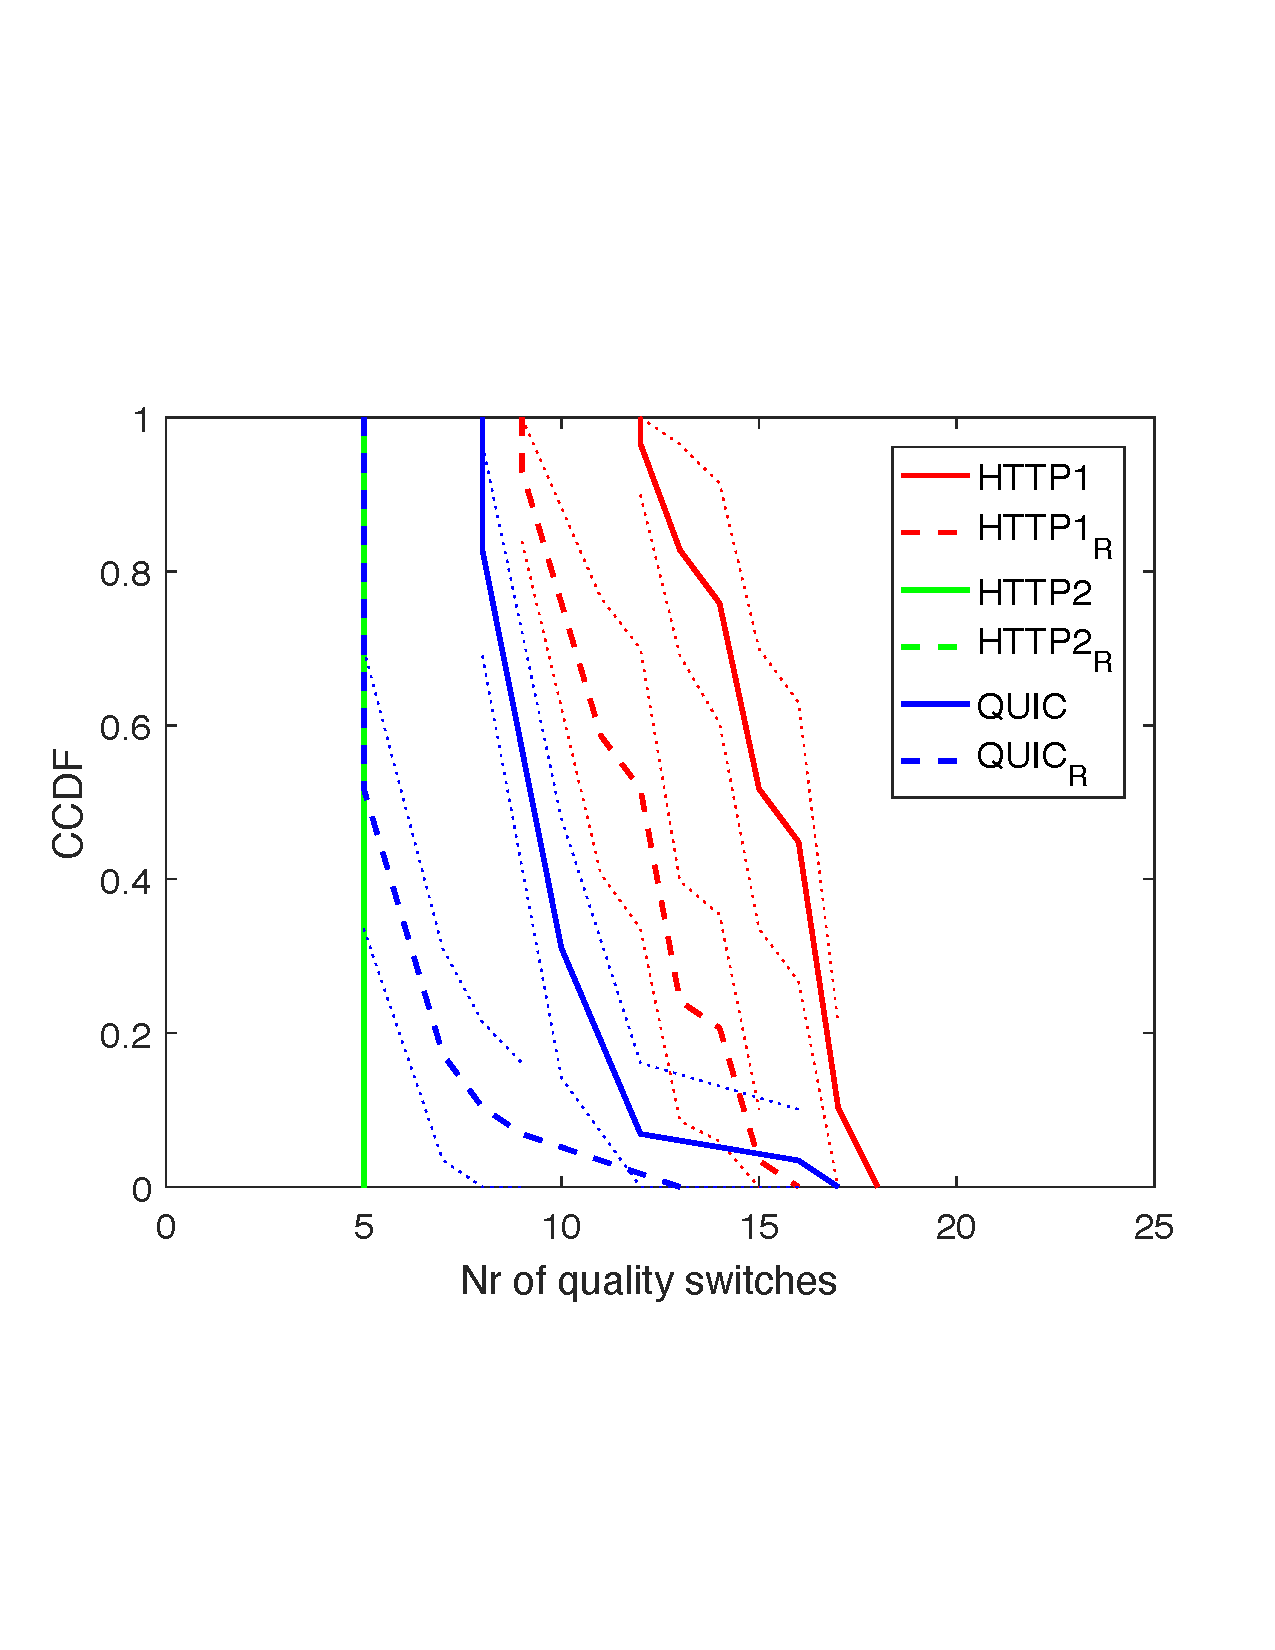
\includegraphics[trim={0 5cm 0 7cm}, scale=0.24]{figures/CDF_cntswitch_squad_udpw9_nd18.pdf}
    \caption{}
    \label{fig:udpw9cntsw}
  \end{subfigure}
  \begin{subfigure}[t]{0.33\textwidth}
  \captionsetup{justification=centering,margin=1.5cm}
    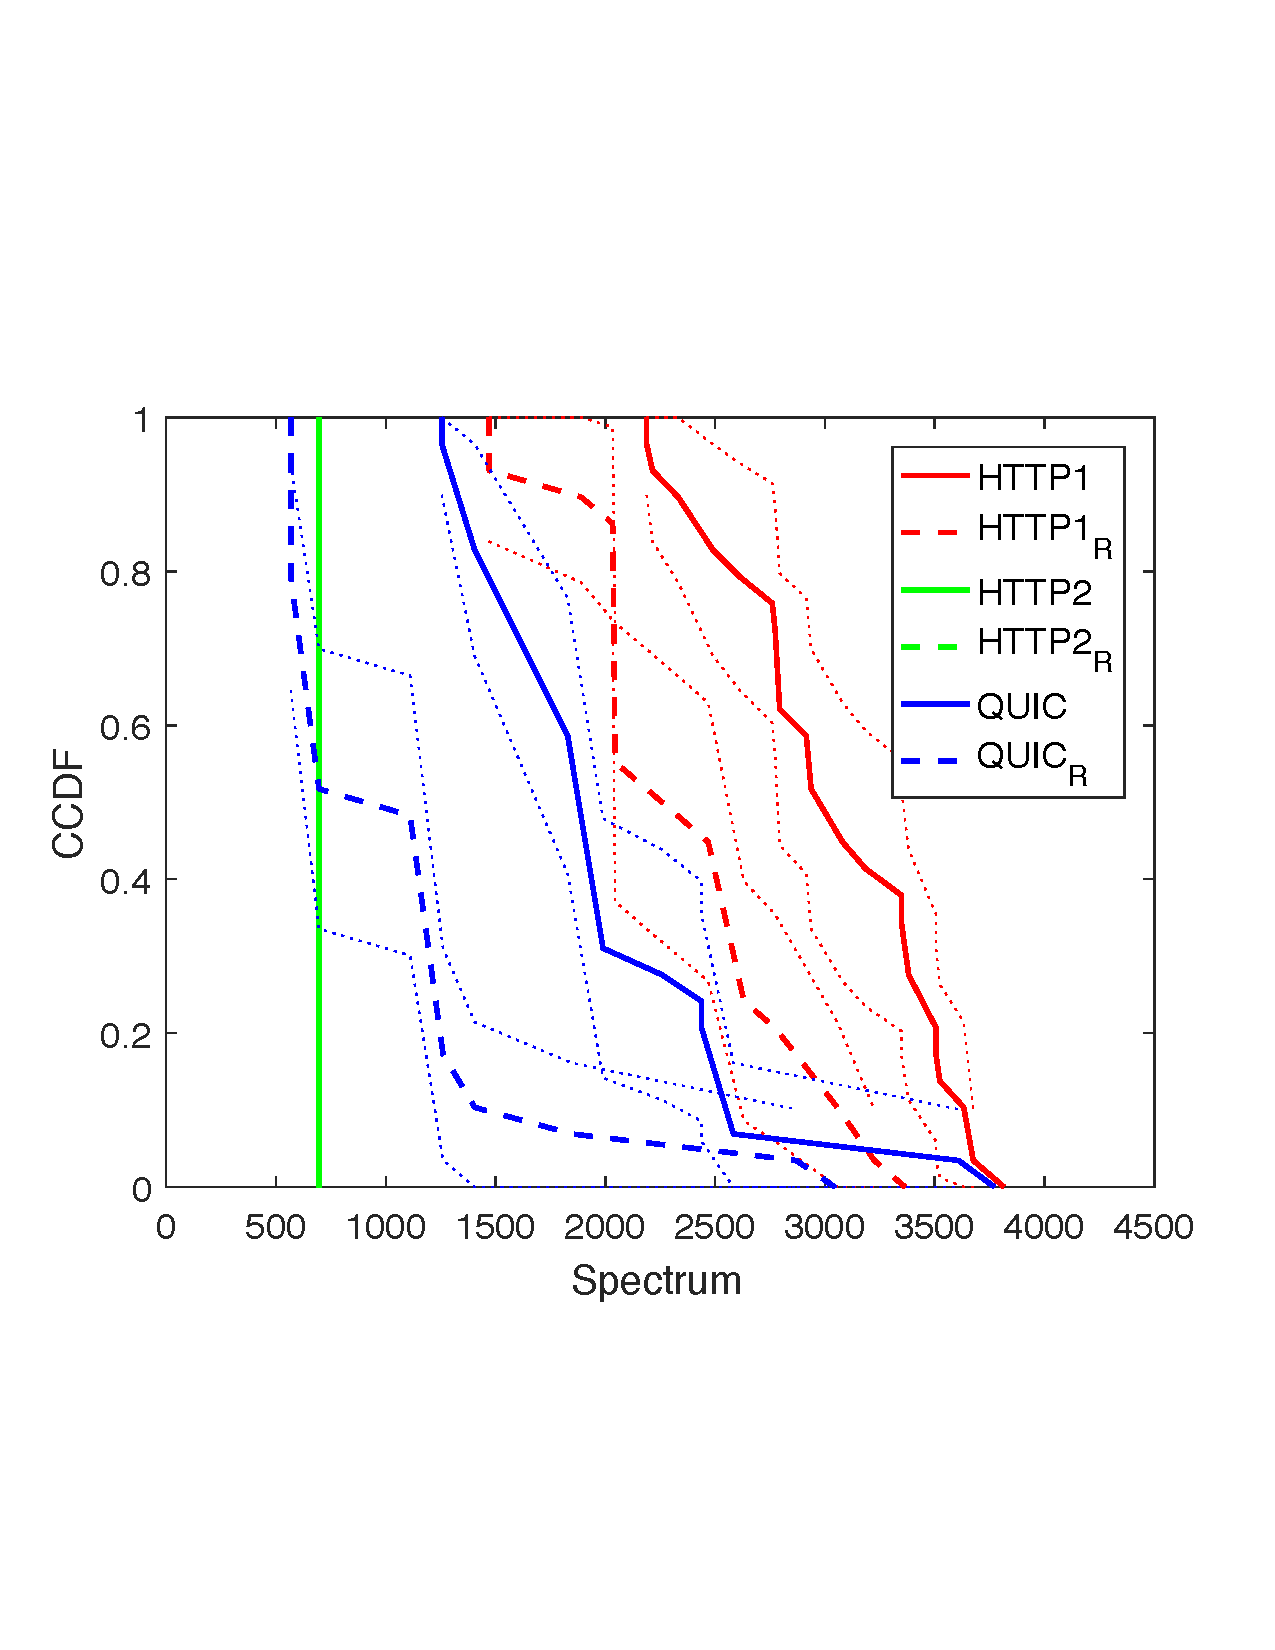
\includegraphics[trim={0 5cm 0 7cm}, scale=0.24]{figures/CDF_magswitch_squad_udpw9_nd18.pdf}
    \caption{}
    \label{fig:udpw9magsw}
  \end{subfigure}
 \centering
  \vspace{-12pt}
  \caption{Single Client Measurements - Rate Limited with UDP-W cross traffic. 
  % Here, we see results of using UDP with a "W" shaped bandwidth as cross traffic varying in amplitude between 9Mbps and 5Mbps. 
  QUIC has a significantly better overall QoE compared to HTTP/1.1. Although HTTP/2 sessions appear to be having a higher QoE, all clients experience 4\% rebuffering. Note, subscript ``R'' denotes ABR segment retransmissions.}
  \label{fig:udpw9}
   \vspace{-15pt}
\end {figure*}

\subsubsection{Single Client: Re-ordering and HOL}
\label{subsubsec:hol}
\begin{figure*}[htb!]
\centering
\begin{subfigure}[t]{0.33\textwidth}
   \captionsetup{justification=centering,margin=0.5cm}
    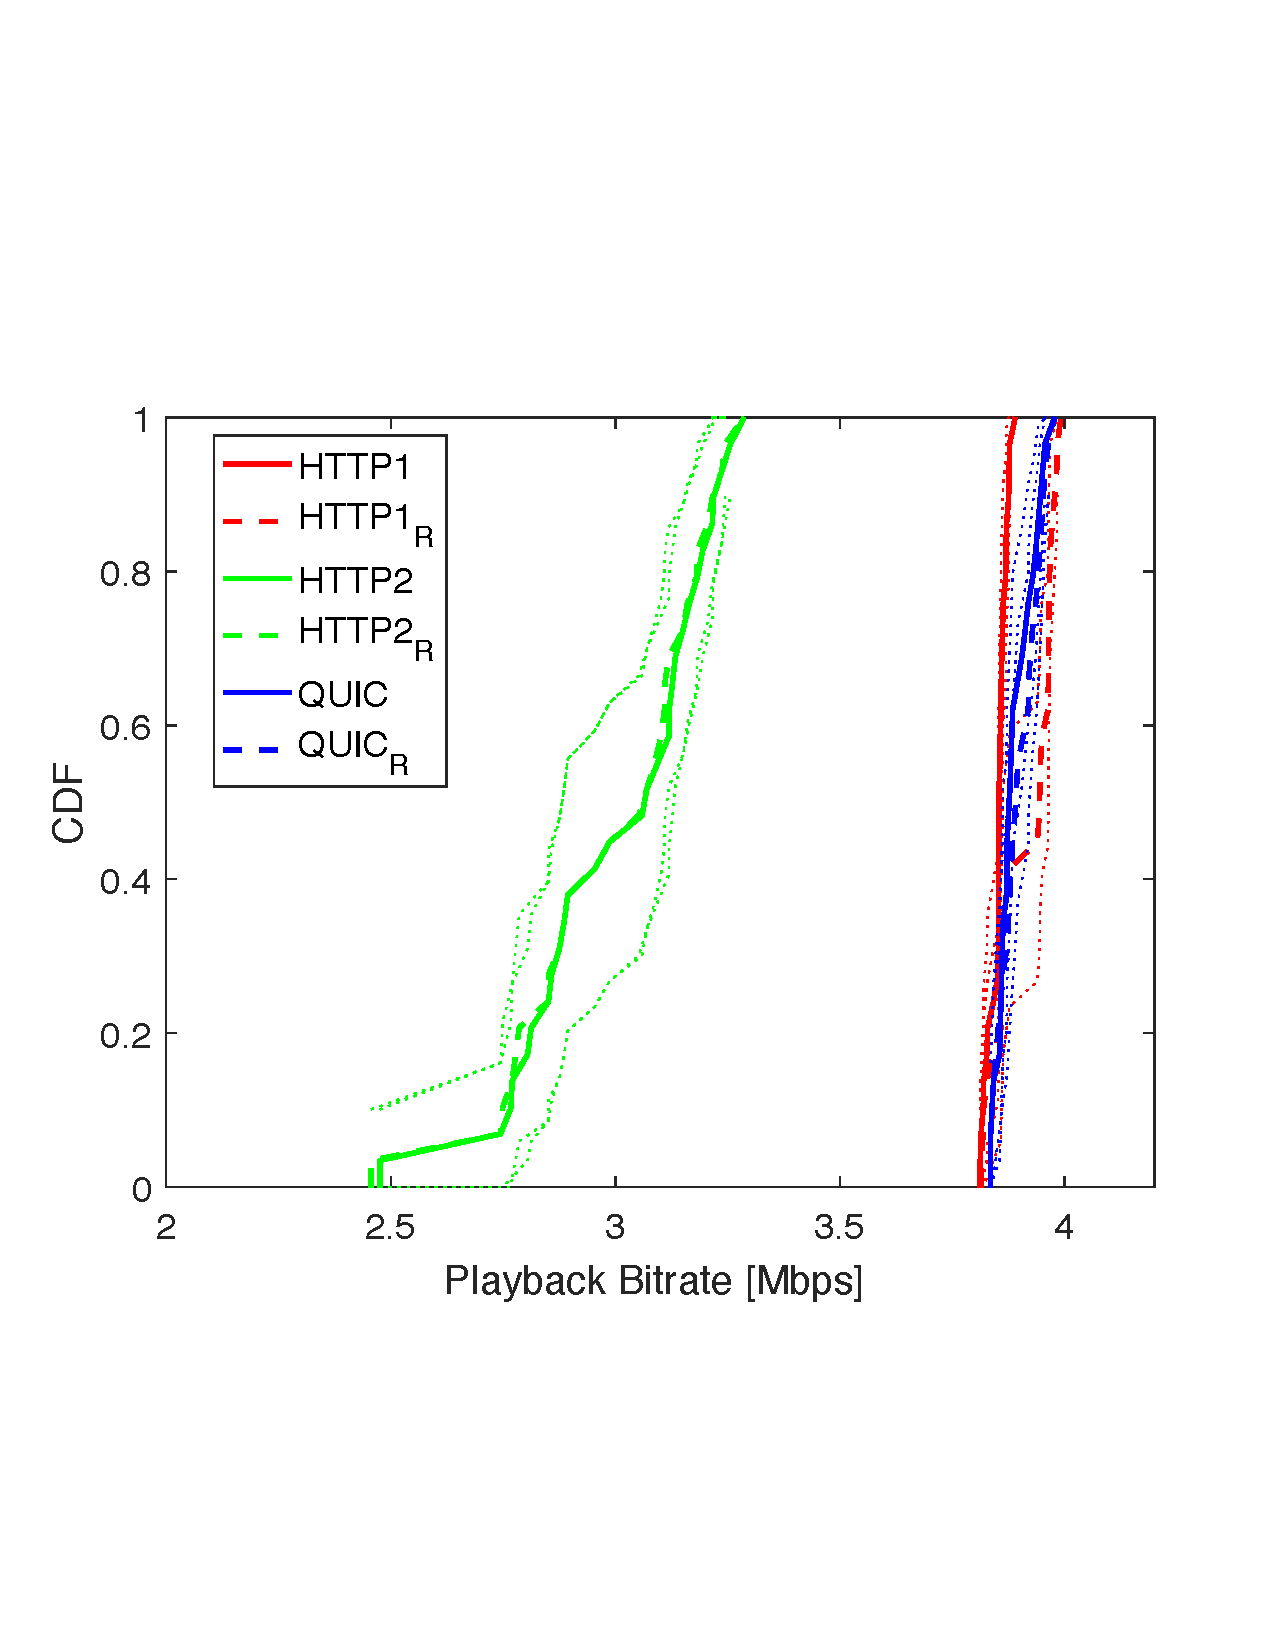
\includegraphics[trim={0 5cm 0 7cm}, scale=0.246]{figures/CDF_bitrat_squad_sdn_p1p2_nd18.pdf}
     \caption{}
    \label{fig:sdn_p1_p2bitrate}
  \end{subfigure}
  \begin{subfigure}[t]{0.33\textwidth}
  \captionsetup{justification=raggedright,singlelinecheck=false,margin=2.5cm}
    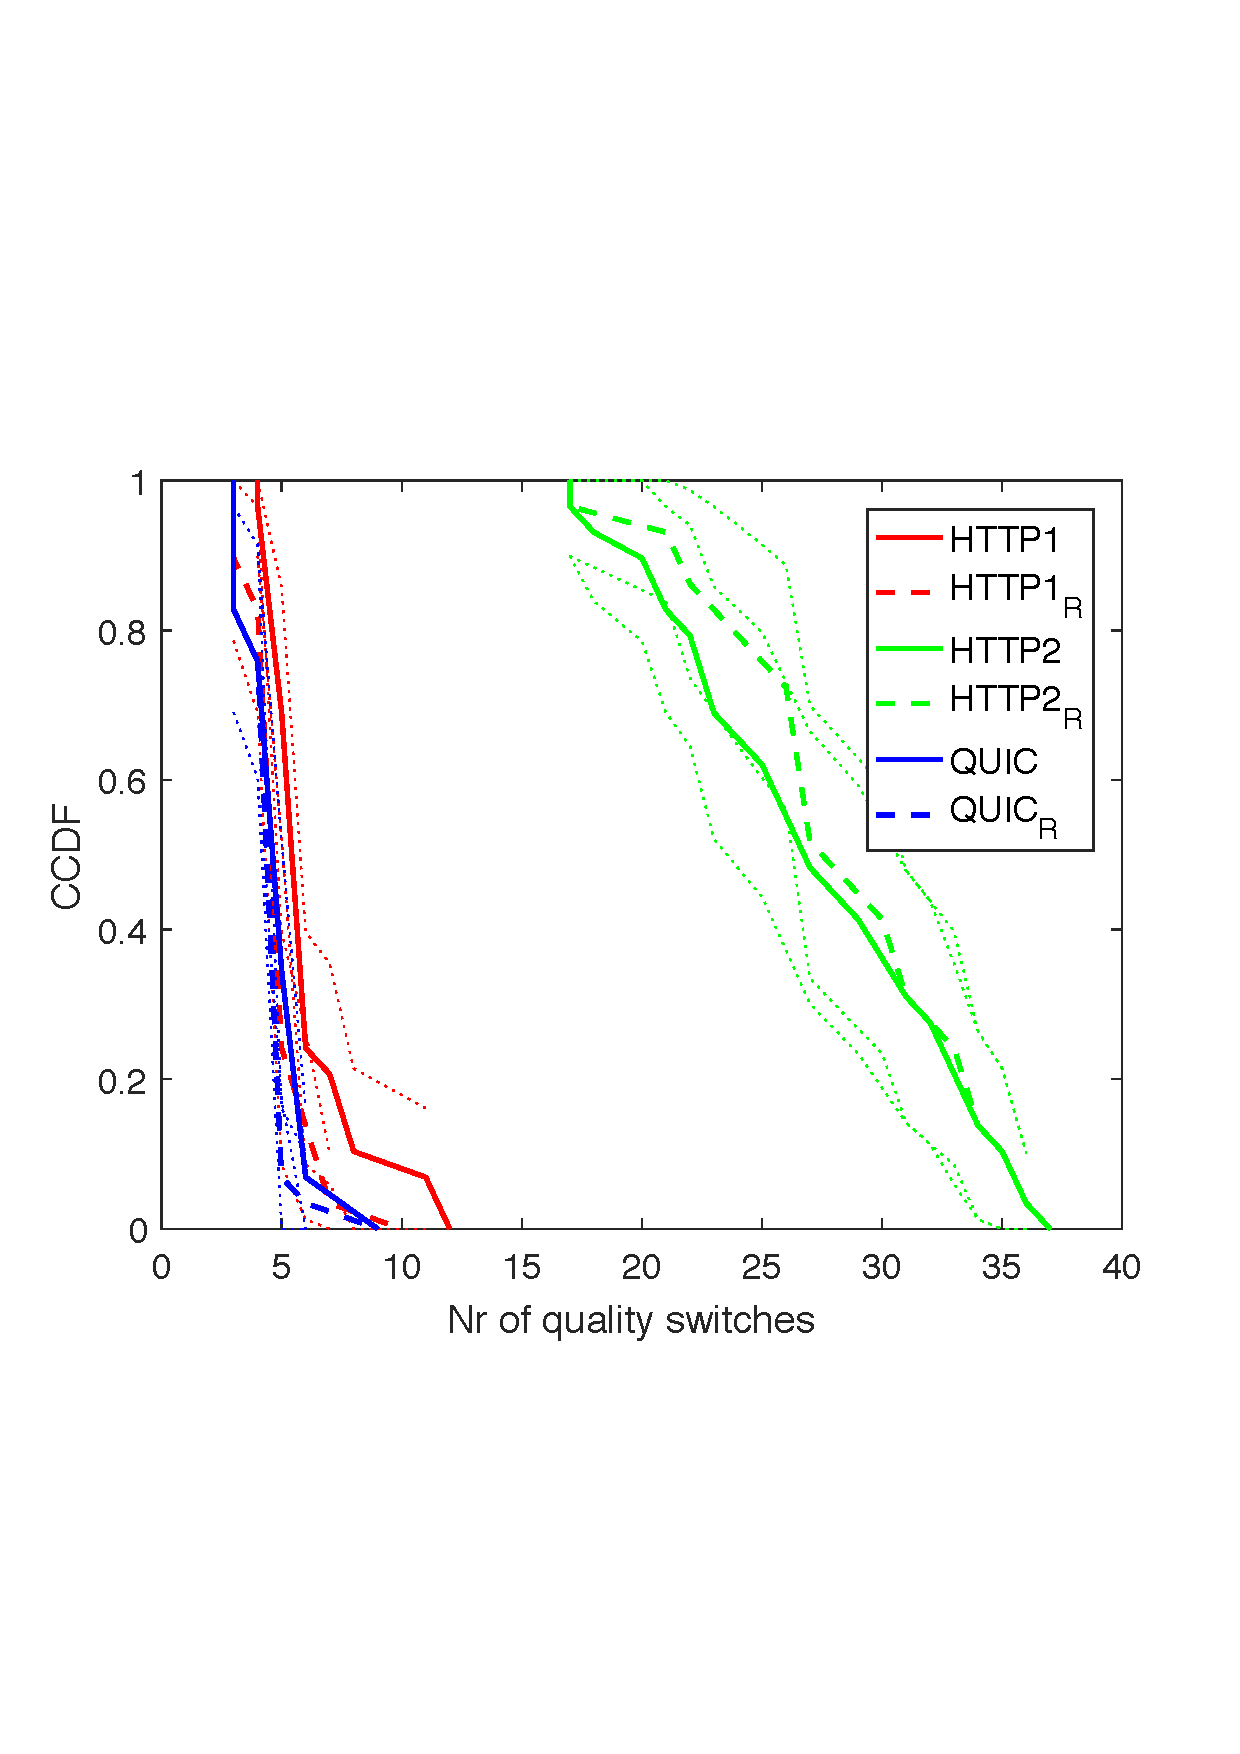
\includegraphics[trim={0 6cm 0 7cm}, scale=0.25]{figures/CDF_cntswitch_squad_sdn_p1p2_nd18.pdf}
    \caption{}
    \label{fig:sdn_p1_p2cntsw}
  \end{subfigure}
 % \begin{subfigure}[t]{0.4\textwidth}
  %\captionsetup{justification=centering,margin=0.5cm}
    %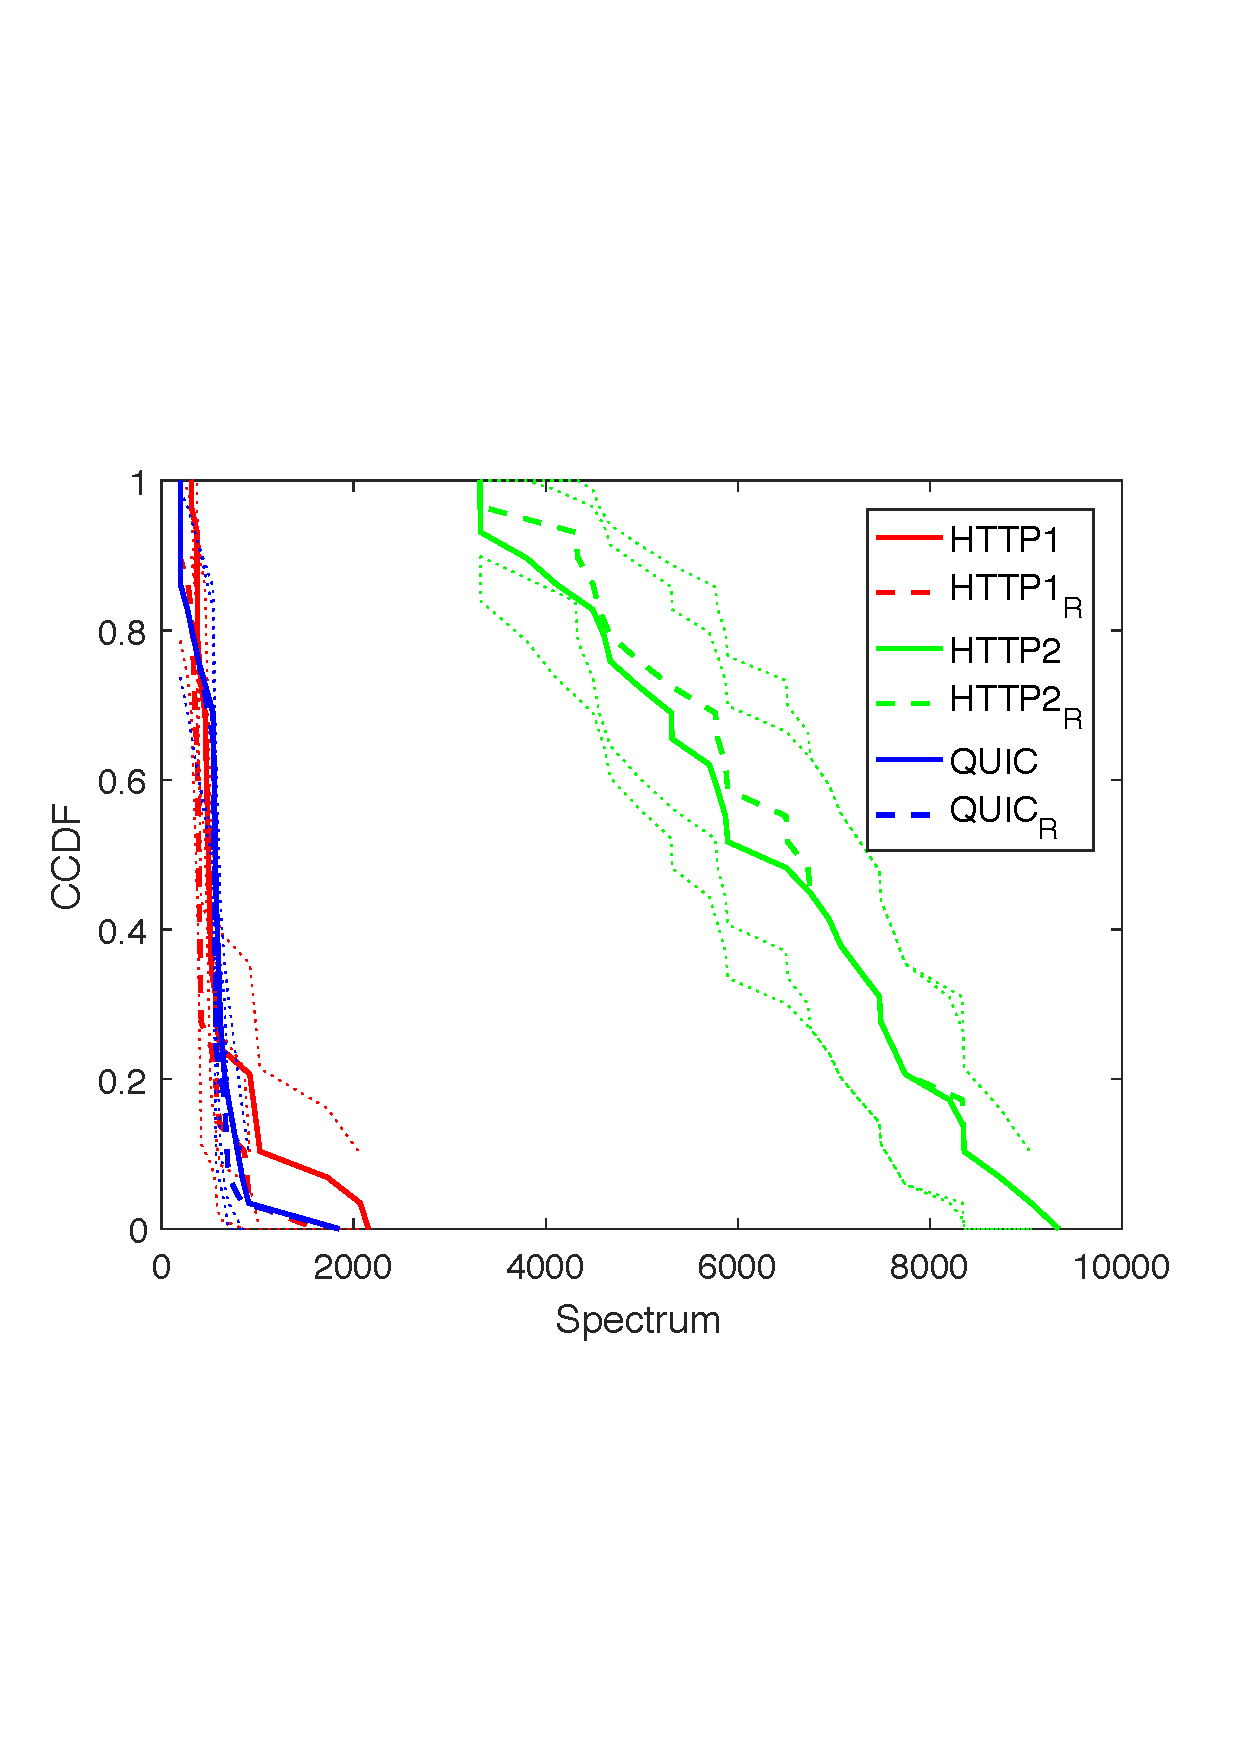
\includegraphics[trim={0 7cm 0 7cm}, scale=0.30]{figures/CDF_magswitch_squad_sdn_p1p2_nd18.pdf}
    %\caption{}
    %\label{fig:sdn_p1_p2magsw}
  %\end{subfigure}
    \begin{subfigure}[t]{0.33\textwidth}
  \captionsetup{justification=centering,margin=1.5cm}
    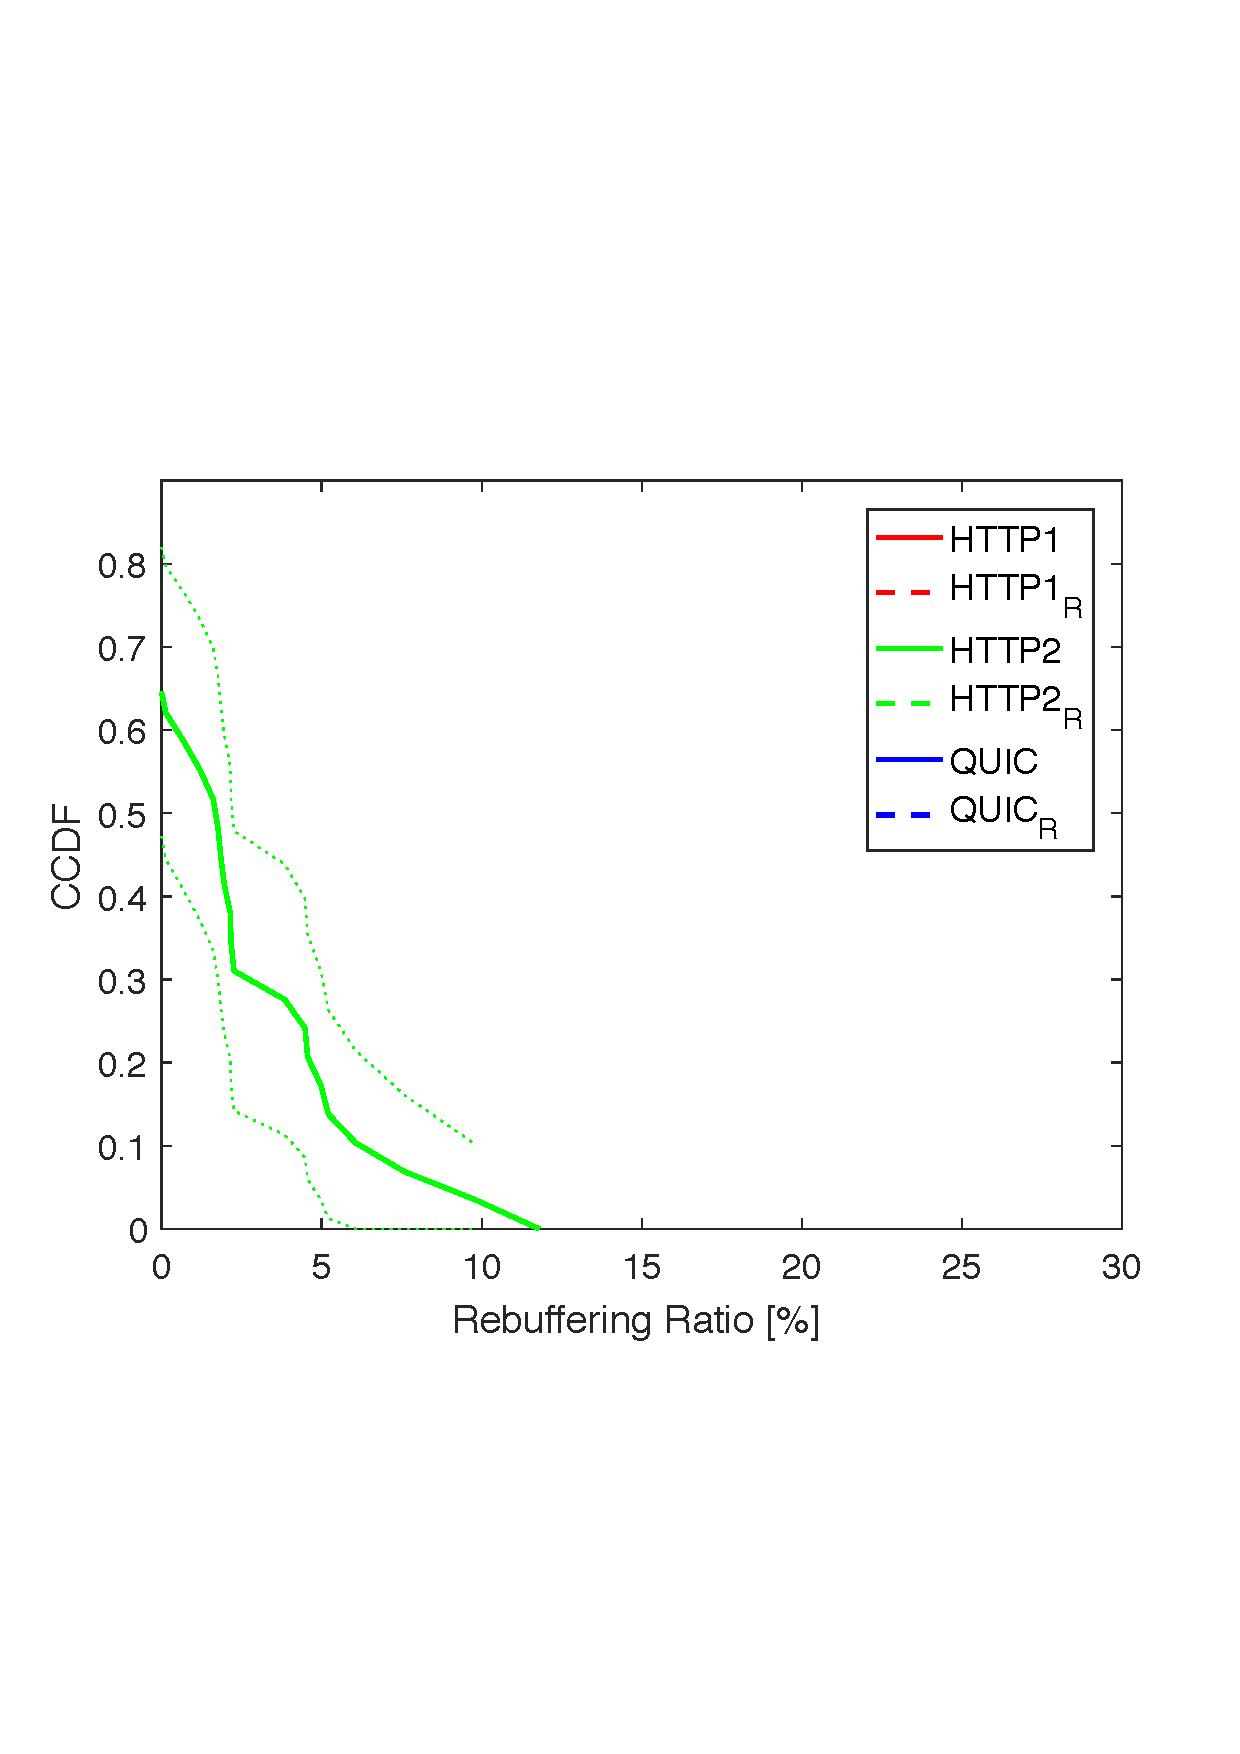
\includegraphics[trim={0 6cm 0 7cm}, scale=0.25]{figures/CDF_rebuffer_squad_sdn_p1p2_nd18.pdf}
    \caption{}
    \label{fig:sdn_p1_p2rebuf}
  \end{subfigure}
 \centering
  \vspace{-20pt}
  \caption{Single Client Measurements - Re-ordering and Head-of-Line Blocking. Re-ordering has an adverse effect on HTTP/2 causing significant degradation of QoE metrics, especially with respect to rebuffering which can be as high as 10\% in spite of selecting lower quality bitrates as seen from (a). Note, subscript ``R'' denotes ABR segment retransmissions.}
  \label{fig:sdn_p1_p2}
  \vspace{-10pt}
\end {figure*}
\ifdefined\flagTech
\begin{figure*}[htb!]
\centering
\begin{subfigure}[t]{0.35\textwidth}
   \captionsetup{justification=centering,margin=0cm}
     \hspace{-55pt}
    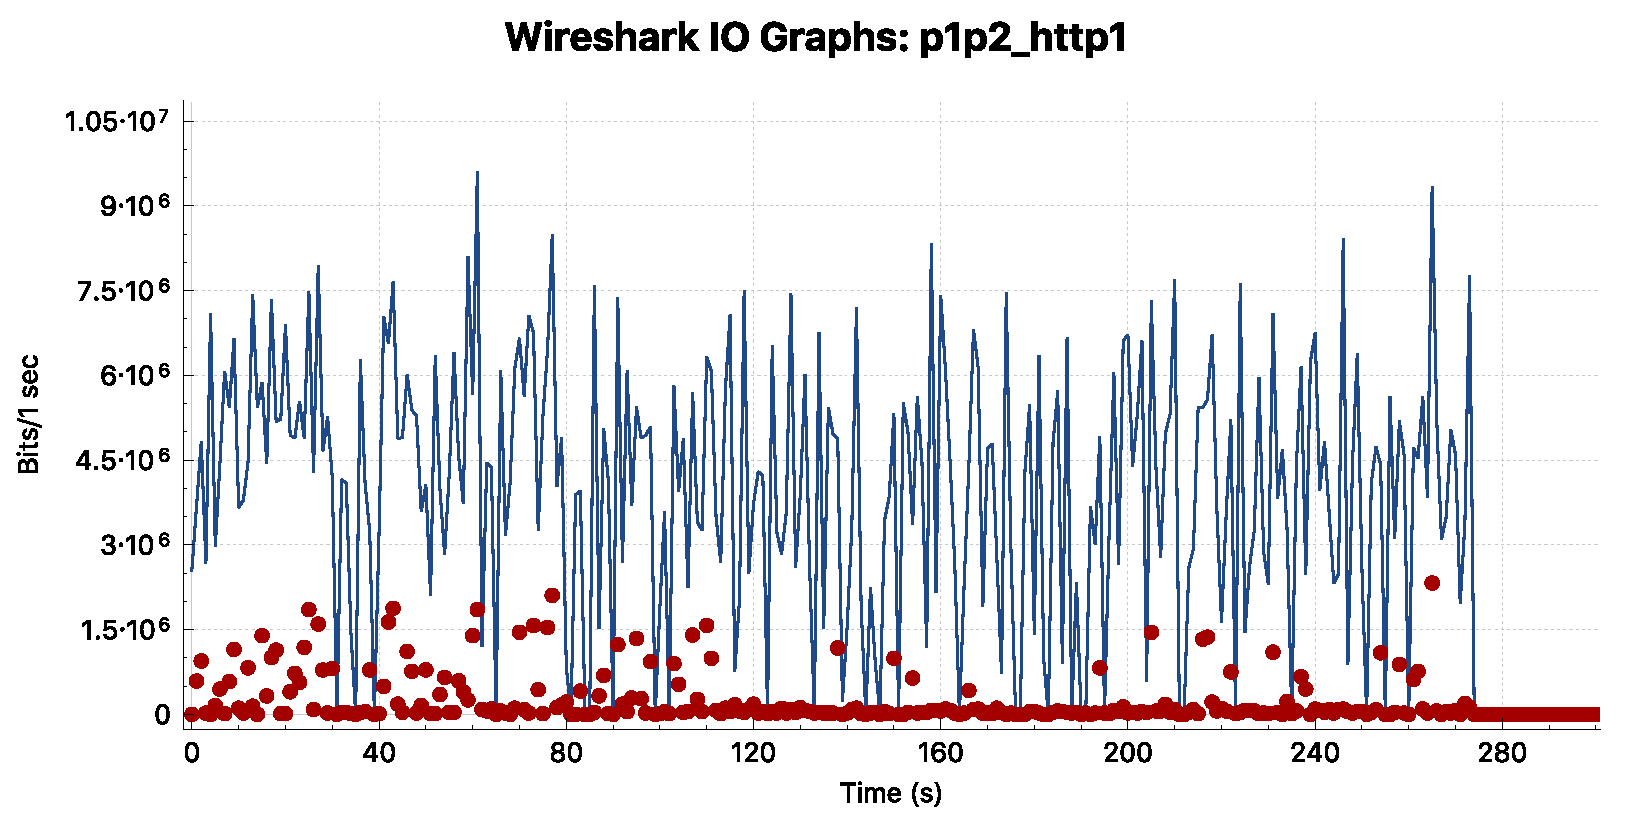
\includegraphics[scale=0.33, trim={100 0 0 0}]{figures/p1p2_http1.pdf}
     \caption{}
    \label{fig:sdn_p1_p2http1}
  \end{subfigure}
  \begin{subfigure}[t]{0.35\textwidth}
  \captionsetup{justification=raggedright,singlelinecheck=false,margin=2.5cm}
    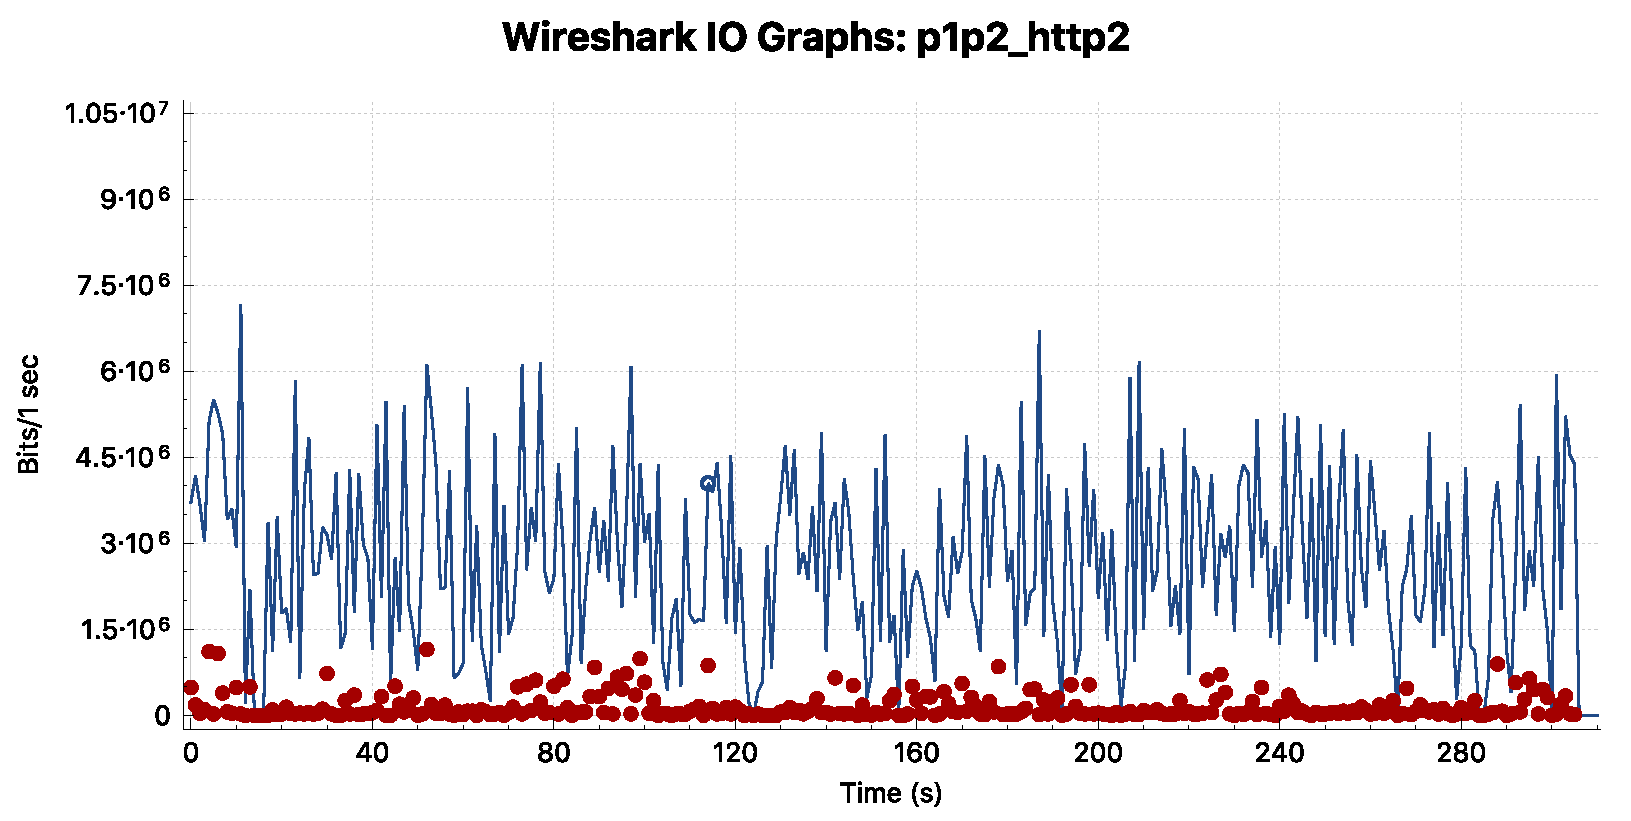
\includegraphics[scale=0.33, trim={25 0 0 0}]{figures/p1p2_http2.pdf}
    \caption{}
    \label{fig:sdn_p1_p2http2}
  \end{subfigure}
    \begin{subfigure}[t]{0.35\textwidth}
  \captionsetup{justification=centering,margin=1.5cm}
    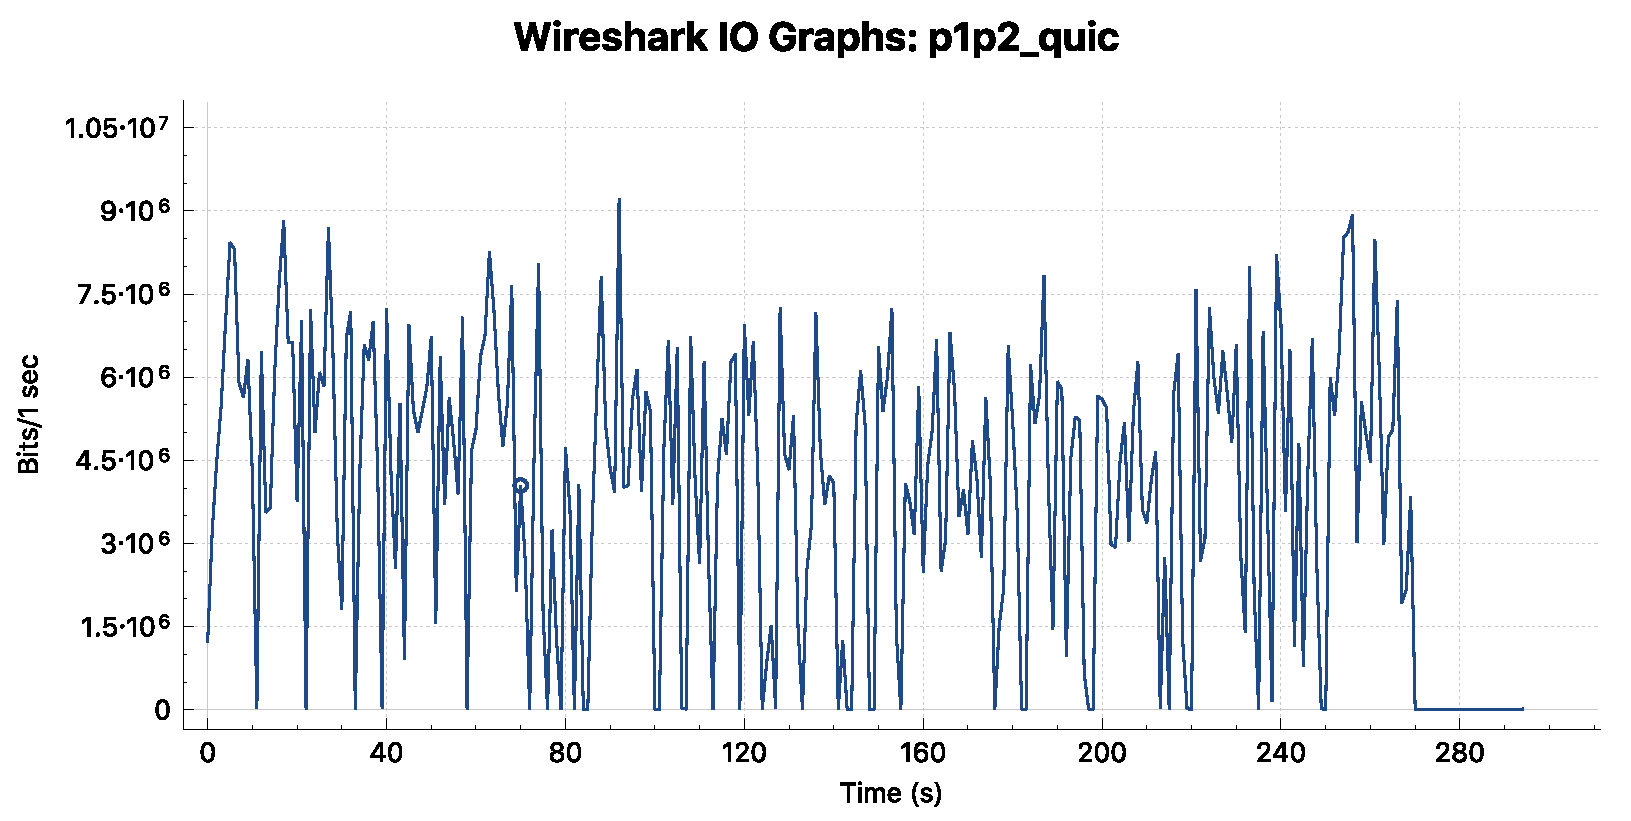
\includegraphics[scale=0.33,trim={150 0 0 0}]{figures/p1p2_quic.pdf}
    \caption{}
    \label{fig:sdn_p1_p2quic}
  \end{subfigure}
 \centering
  \caption{Single Client Measurements - Re-ordering and Head-of-Line Blocking. \texttt{Tshark} traces for one sample show that HTTP1.1 and HTTP2 experience significant TCP fast retransmits which cause QoE degradation when compared to QUIC.}
  \label{fig:sdn_p1_p2_wireshark}
 \vspace{-10pt}
\end {figure*}
\fi
Since packet reordering in the Internet is not uncommon~\cite{Jaiswal:TON:2007}, protocols for ABR streaming should be robust in the face of such reordering. Here, we study the ability of HTTP1.1, HTTP/2, and QUIC to recover from re-ordering of packets. This is the only experiment where we use the second path (denoted \textbf{P2} in Fig. \ref{fig:clab_topo}) to carry video streams. In order to induce re-ordering of packets, we switch between a low latency, low loss path, \textbf{P1}, and a high latency, high loss path, \textbf{P2}, every second using SDN, namely the OpenFlow \cite{mckeown2008openflow} implementation, which provides fine-grained, dynamic traffic engineering for application packets. As shown in Fig. \ref{fig:clab_topo}, \textbf{P2} is characterized by 1\% loss and 10ms delay implemented using \texttt{tc}\footnote{\url{http://lartc.org/manpages/tc.txt}} and \texttt{netem}\footnote{\url{http://man7.org/linux/man-pages/man8/tc-netem.8.html}} utilities. For the experiments presented in Sect.~\ref{subsubsec:single_udp}, we find that HTTP/2 is either comparable or marginally worse than HTTP/1.1 and QUIC. In the case of packet reordering (shown in Figure \ref{fig:sdn_p1_p2}), we see that HTTP/2 performs significantly worse than QUIC and HTTP/1.1 . Not only is the $AQB$ significantly lower with a high variation between runs, but also the rebuffering is as high as 10\% where over 60\% of clients experience an $RB$ of ~2.5\%. Further analysis using the \texttt{tshark}\footnote{\url{https://www.wireshark.org/docs/man-pages/tshark.html}} utility reveals that a HTTP/2 session experiences 9.5\% fast TCP retransmits. In comparison, HTTP/1.1 experiences 7.1\%, and QUIC sessions experience no UDP retransmissions since they use NACKs (c.f. Sect. \ref{subsubsec:quicvstcp}). More details on the \texttt{tshark} data can be found in~\cite{QUIC_TR:2018}
\ifdefined\flagTech \DB{Fig. \ref{fig:sdn_p1_p2_wireshark}. Here, we take the example of one run to show that HTTP1.1 and HTTP/2 experience several fast retransmits as compared to QUIC.} \fi Additionally, QUIC uses a higher initial congestion window size=32 (the Linux default for TCP is 10) and also grows the window more aggressively, thus, allowing more unacknowledged bytes in flight. This results in a more reliable download rate measurement and a stable buffer level for the ABR client and consequently, a reduction in the quality variations $\#QS$ as observed in Fig. \ref{fig:sdn_p1_p2cntsw}. 

\subsubsection{Parallel Clients: Competing Traffic}
For this experiment we use the additional client and server pairs (denoted as \textit{Client2}/\textit{Server2} and \textit{Client3}/\textit{Server3} in Figure \ref{fig:clab_topo}) to initiate three simultaneous sessions of QUIC-based SQUAD clients. Although all three clients enjoy a smooth playback experience without rebuffering as shown in Figure \ref{fig:pquic}, we note that the bandwidth sharing can result in unfair behavior in the case of ABR streaming sessions. This is contrary to the analysis presented by the authors of \cite{Kakhki:IMC:2017} where they observe that QUIC flows are fair to each other but only unfair to TCP flows when downloading a file. While we similarly observe that QUIC does tend to "starve out" TCP flows, we note that ABR streaming over QUIC with the use of retransmissions can result in unfair behavior for competing ABR streams since multiplexing due to retransmissions can occur at different points throughout the streaming session. In order to corroborate this analysis, we present the percentage of retransmissions in Table \ref{tab:retx_parallel_quic}, which shows that the three clients experience varying number of ABR segment retransmissions per run. Since these retransmissions occur asynchronously, the clients observe different buffer levels and rate measurements throughout a streaming session. We also perform similar experiments with three HTTP/2 clients and observe that HTTP/2 shows a nearly equal distribution of $AQB$ and closer inspection reveals that the $AQB$ of \textit{Client1} is 0.5Mbps higher on average as compared to the other two clients. Since TCP is more conservative about setting the initial congestion window size and has a less aggressive window growth it enables all three clients to have a "fair" share of the bottleneck bandwidth. Further details on the TCP-based experiments can be found in~\cite{QUIC_TR:2018}.
\ifdefined\flagTech \DB{Figure \ref{fig:phttp1} shows the QoE metrics for a case with three concurrent ABR clients and Figure \ref{fig:phttp2} shows similar results for three parallel HTTP/2 clients. Although none of the clients experience rebuffering in both cases, for HTTP1.1 clients, we see that one client obtains a very high bitrate compared to the others. Since the retransmissions do not occur simultaneously with original segment downloads in the HTTP1.1 case, we note that this creates significant heterogeneity in the bitrate of sequential requests made by various clients. We do not observe such an affect in the case of HTTP/2 since the retransmissions are multiplexed with original segments and TCP naturally ensures fairness. After understanding the concurrent behavior of HTTP1.1, HTTP2 and QUIC individually, we present one case where each of these three protocols compete with each other in Fig. \ref{fig:pmixed} which reveals that  HTTP1.1 and QUIC sessions have a relatively high QoE when compared to HTTP/2 sessions, which experience rebuffering as high as 23\% in addition to low quality bitrates, which leads us to conclude that the multiplexing feature of HTTP/2 is severely limited by underlying TCP parameters that need to be better tuned to support such a feature in order to obtain a better QoE performance.}\fi
\label{subsubsec:parallel}
\begin{figure*}[t!]
\centering
\begin{subfigure}[t]{0.33\textwidth}
   \captionsetup{justification=centering,margin=4.5cm}
    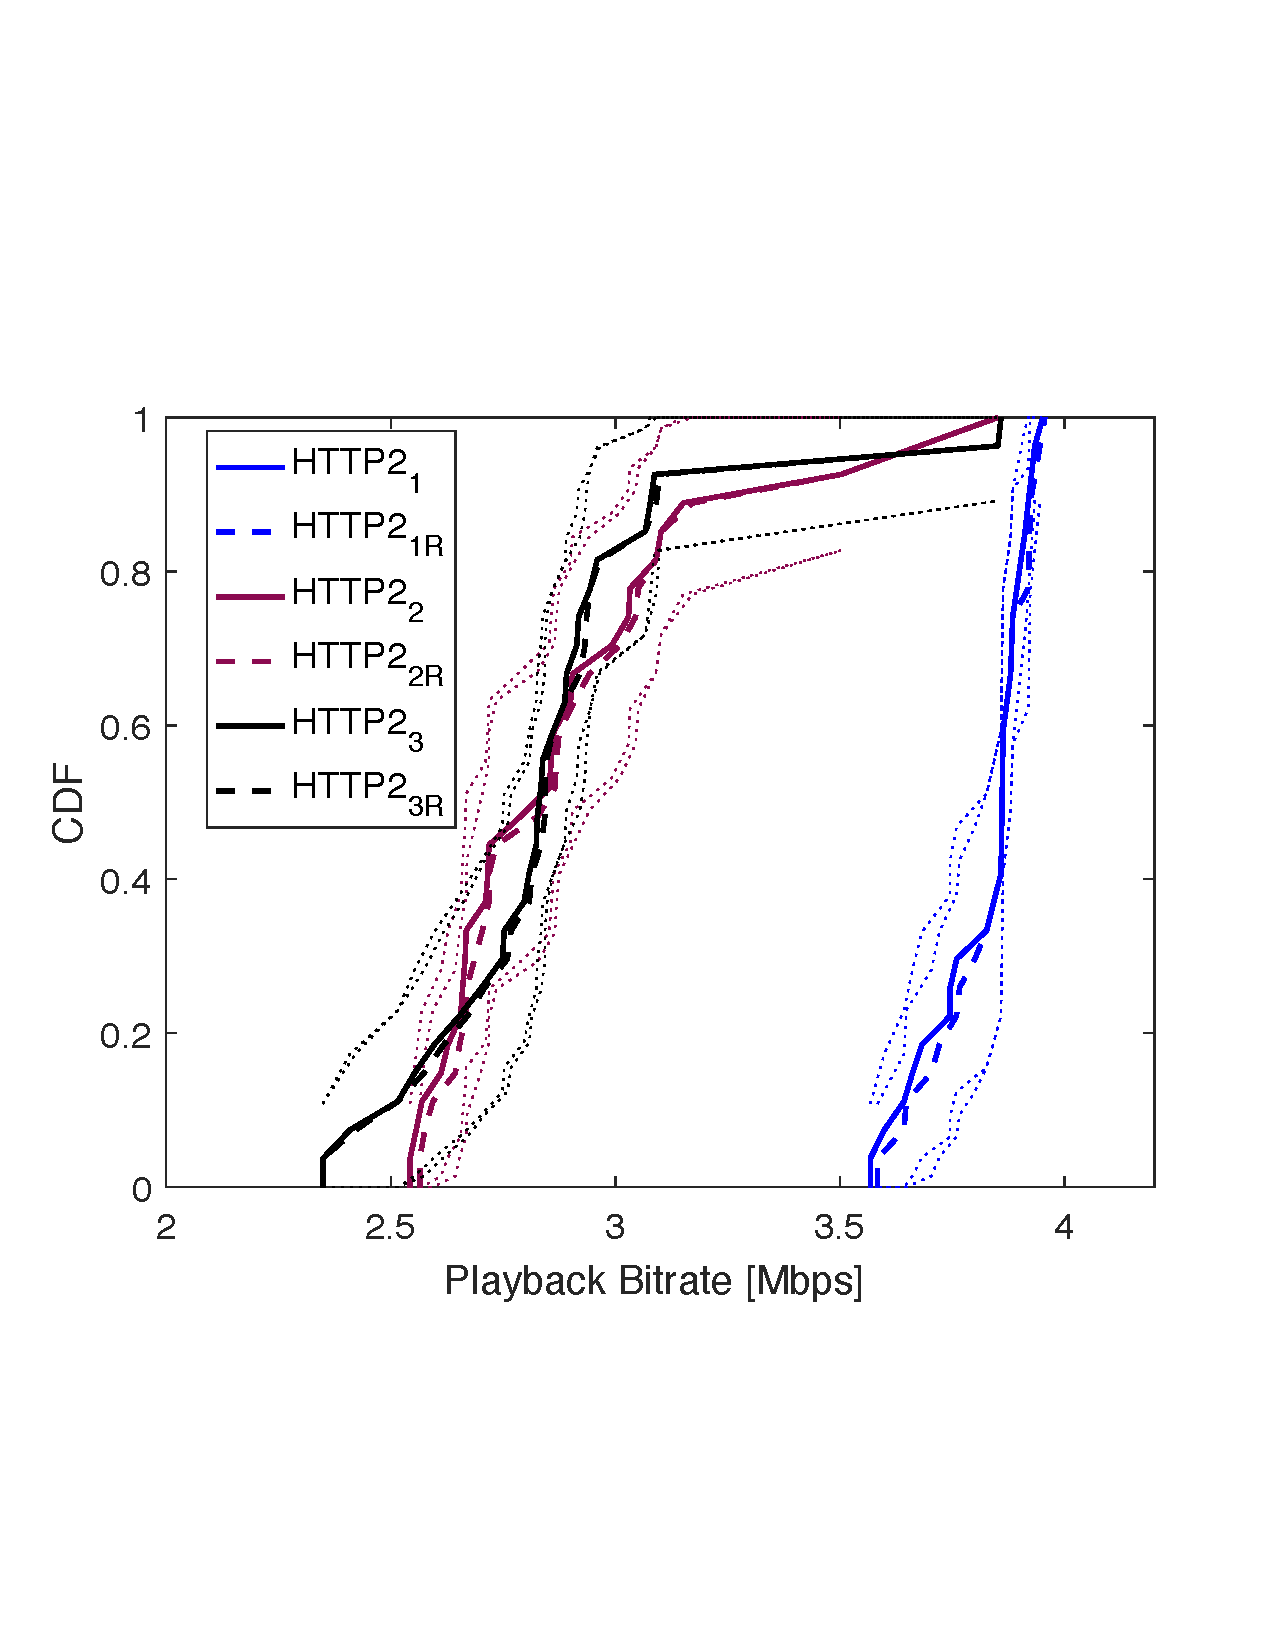
\includegraphics[trim={0 6cm 0 7cm}, scale=0.246]{figures/CDF_bitrat_squad_parallel_quic_nd18.pdf}
     \caption{}
    \label{fig:pquicbitrate}
  \end{subfigure}
  \begin{subfigure}[t]{0.33\textwidth}
  \captionsetup{justification=raggedright,singlelinecheck=false,margin=2.5cm}
    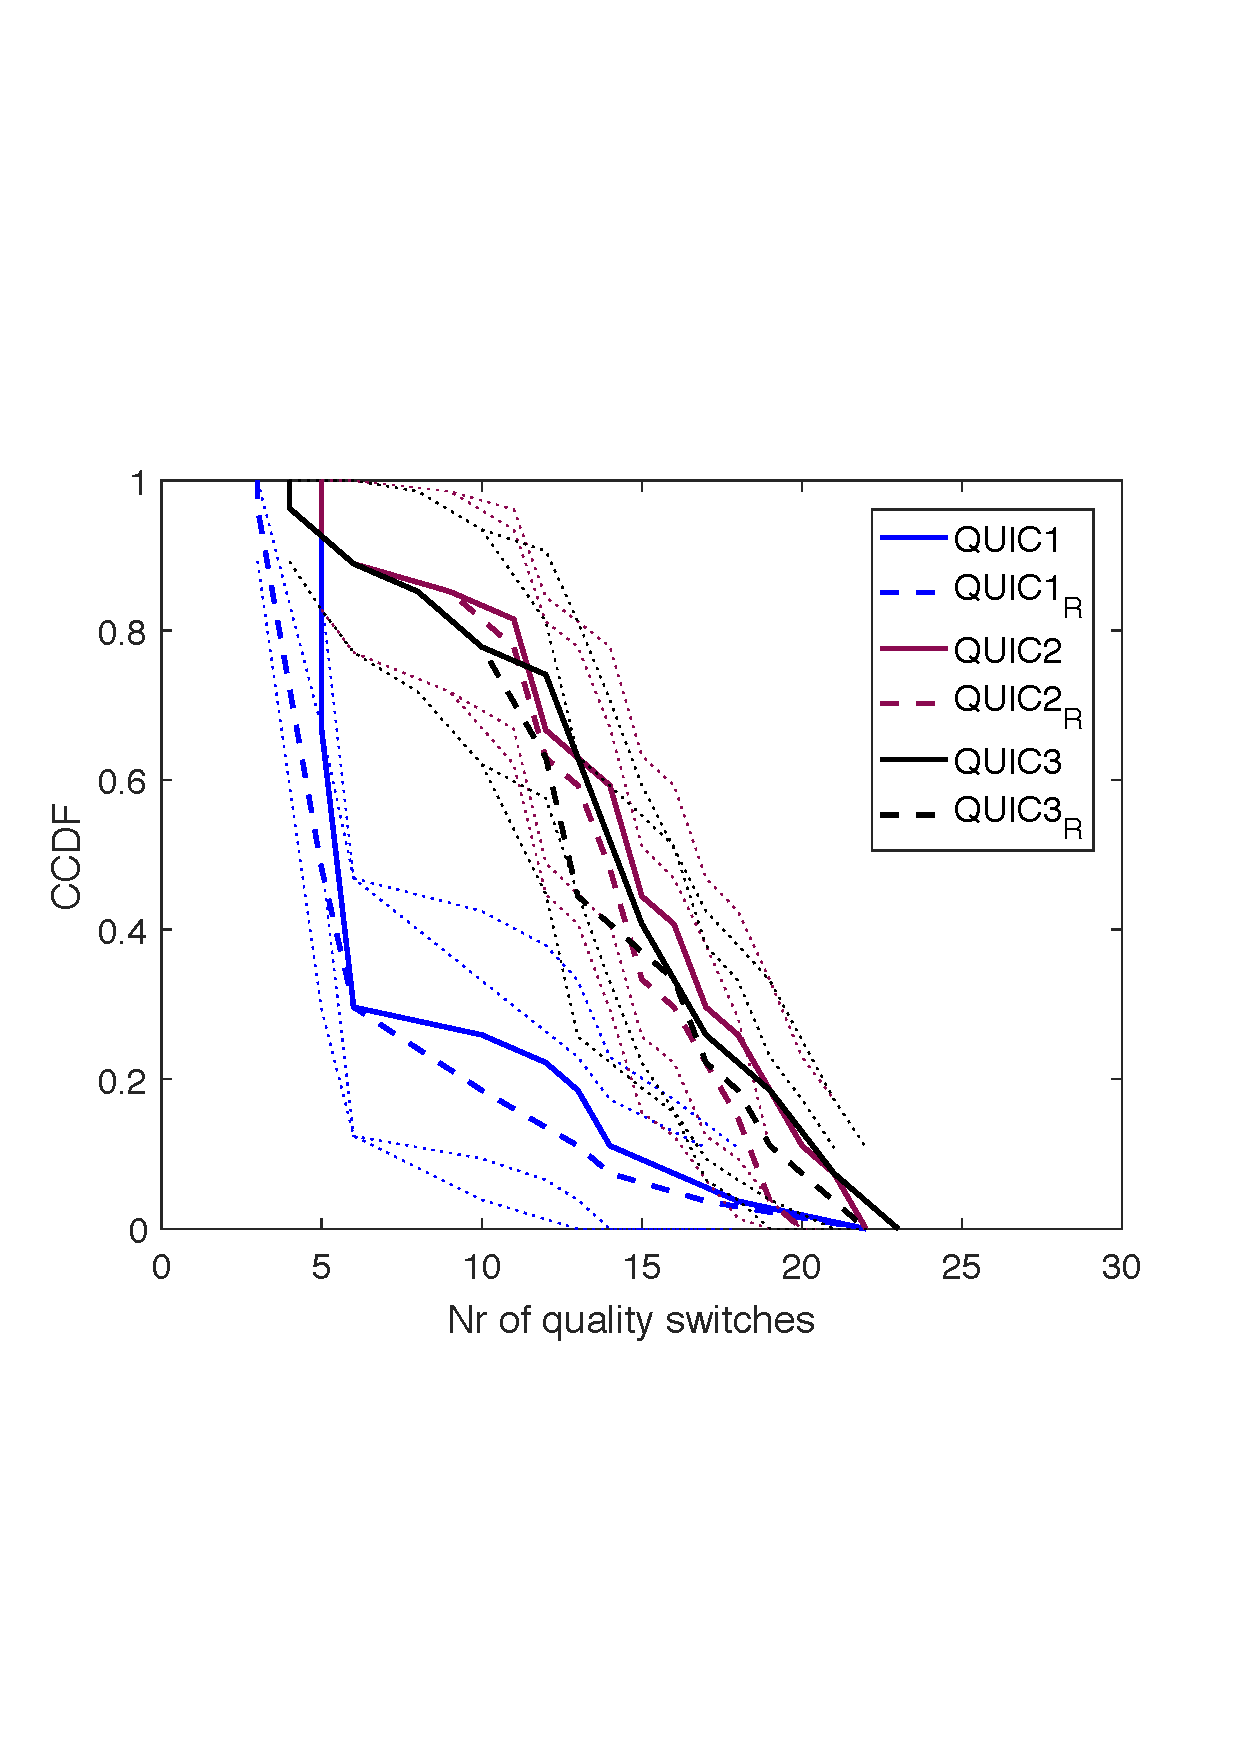
\includegraphics[trim={0 7cm 0 7cm}, scale=0.25]{figures/CDF_cntswitch_squad_parallel_quic_nd18.pdf}
    \caption{}
    \label{fig:pquiccntsw}
  \end{subfigure}
  \begin{subfigure}[t]{0.33\textwidth}
  \captionsetup{justification=centering,margin=1.5cm}
    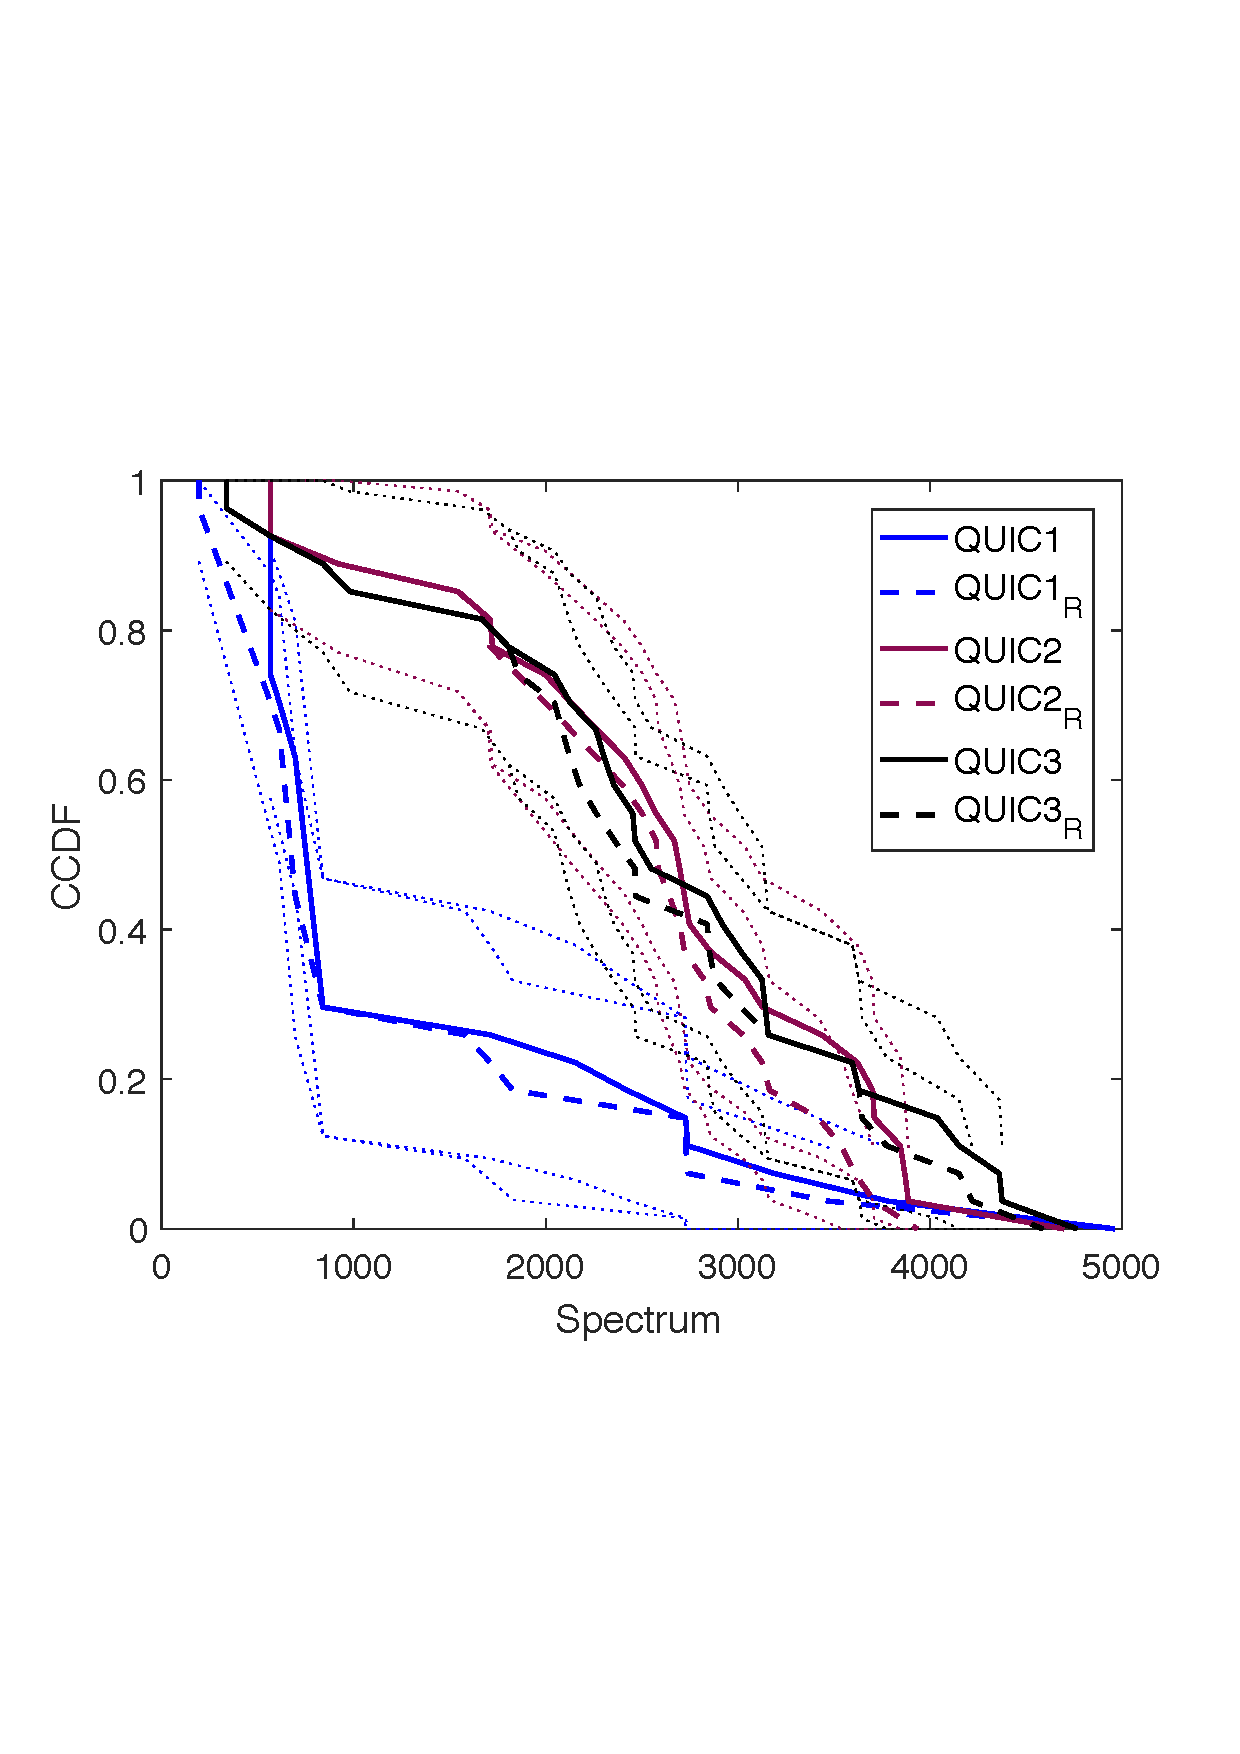
\includegraphics[trim={0 7cm 0 7cm}, scale=0.25]{figures/CDF_magswitch_squad_parallel_quic_nd18.pdf}
    \caption{}
    \label{fig:pquicmagsw}
  \end{subfigure}
 \centering
    \vspace{-15pt}
  \caption{Parallel Client Measurements - Three QUIC Clients. Competing QUIC clients show an unfair behavior where two clients experience relatively similar QoE but one client has a significantly better QoE than others.}
  \label{fig:pquic}
  \vspace{-10pt}
\end {figure*}
\ifdefined\flagTech
\begin{figure*}[t!]
\centering
\begin{subfigure}[t]{0.33\textwidth}
   \captionsetup{justification=centering,margin=4.5cm}
    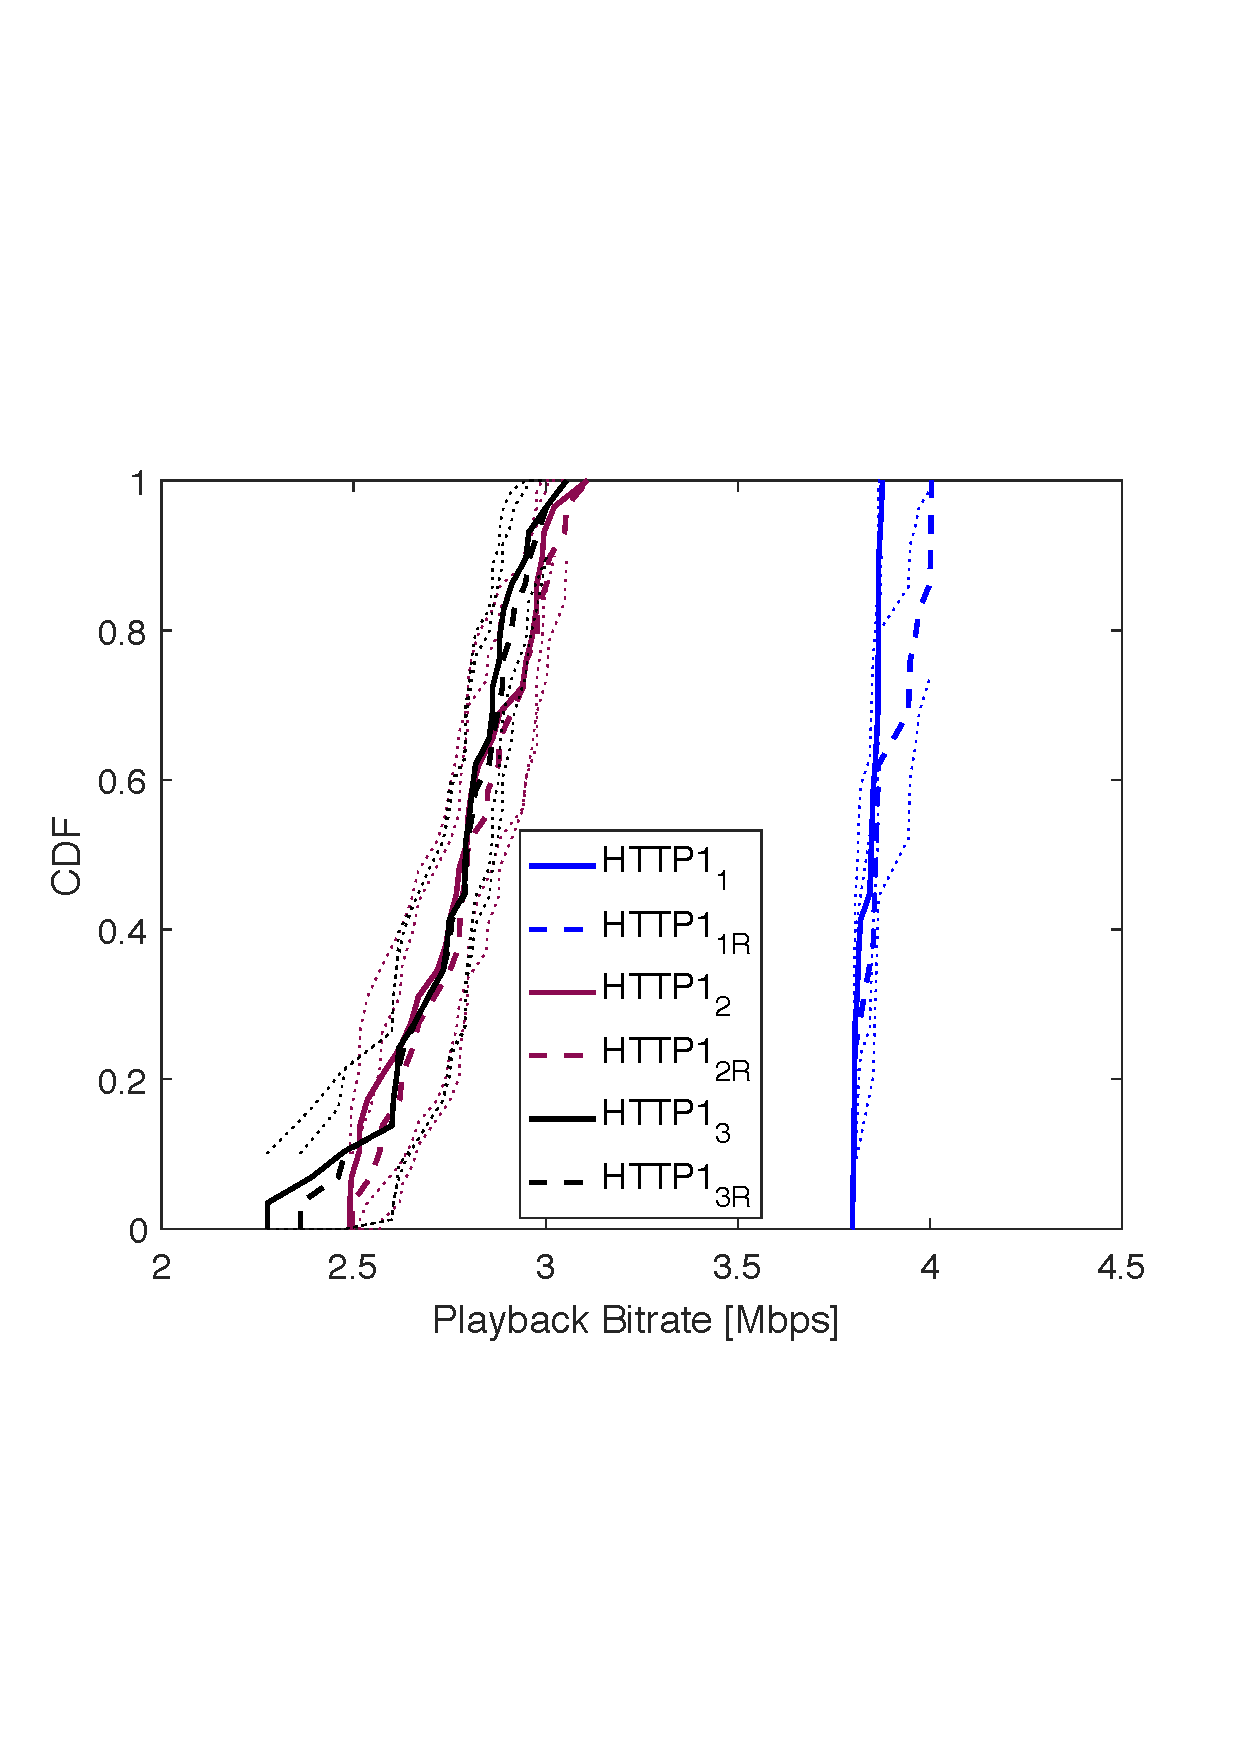
\includegraphics[trim={0 7cm 0 7cm}, scale=0.25]{figures/CDF_bitrat_squad_parallel_http1_nd18.pdf}
     \caption{}
    \label{fig:phttp1bitrate}
  \end{subfigure}
  \begin{subfigure}[t]{0.33\textwidth}
  \captionsetup{justification=raggedright,singlelinecheck=false,margin=2.5cm}
    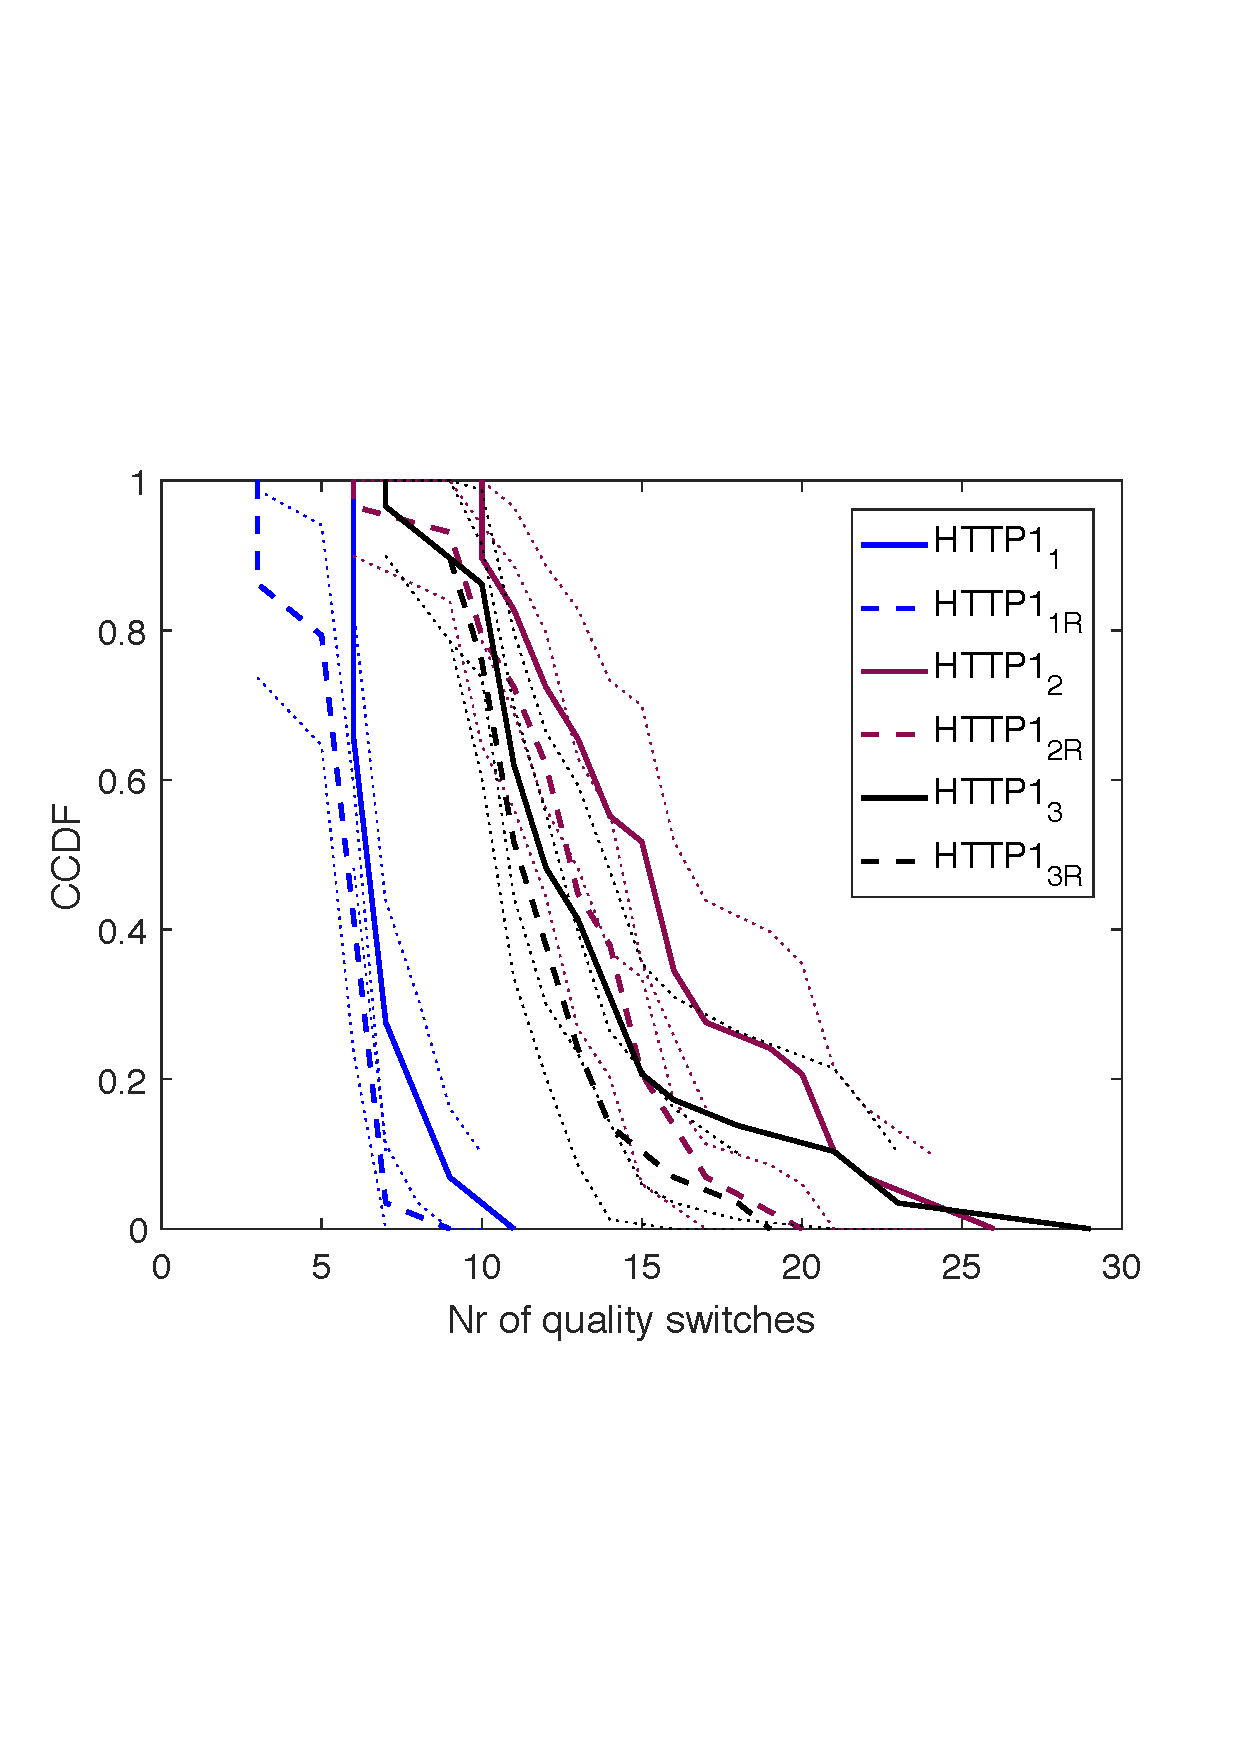
\includegraphics[trim={0 7cm 0 7cm}, scale=0.25]{figures/CDF_cntswitch_squad_parallel_http1_nd18.pdf}
    \caption{}
    \label{fig:phttp1cntsw}
  \end{subfigure}
  \begin{subfigure}[t]{0.33\textwidth}
  \captionsetup{justification=centering,margin=1.5cm}
    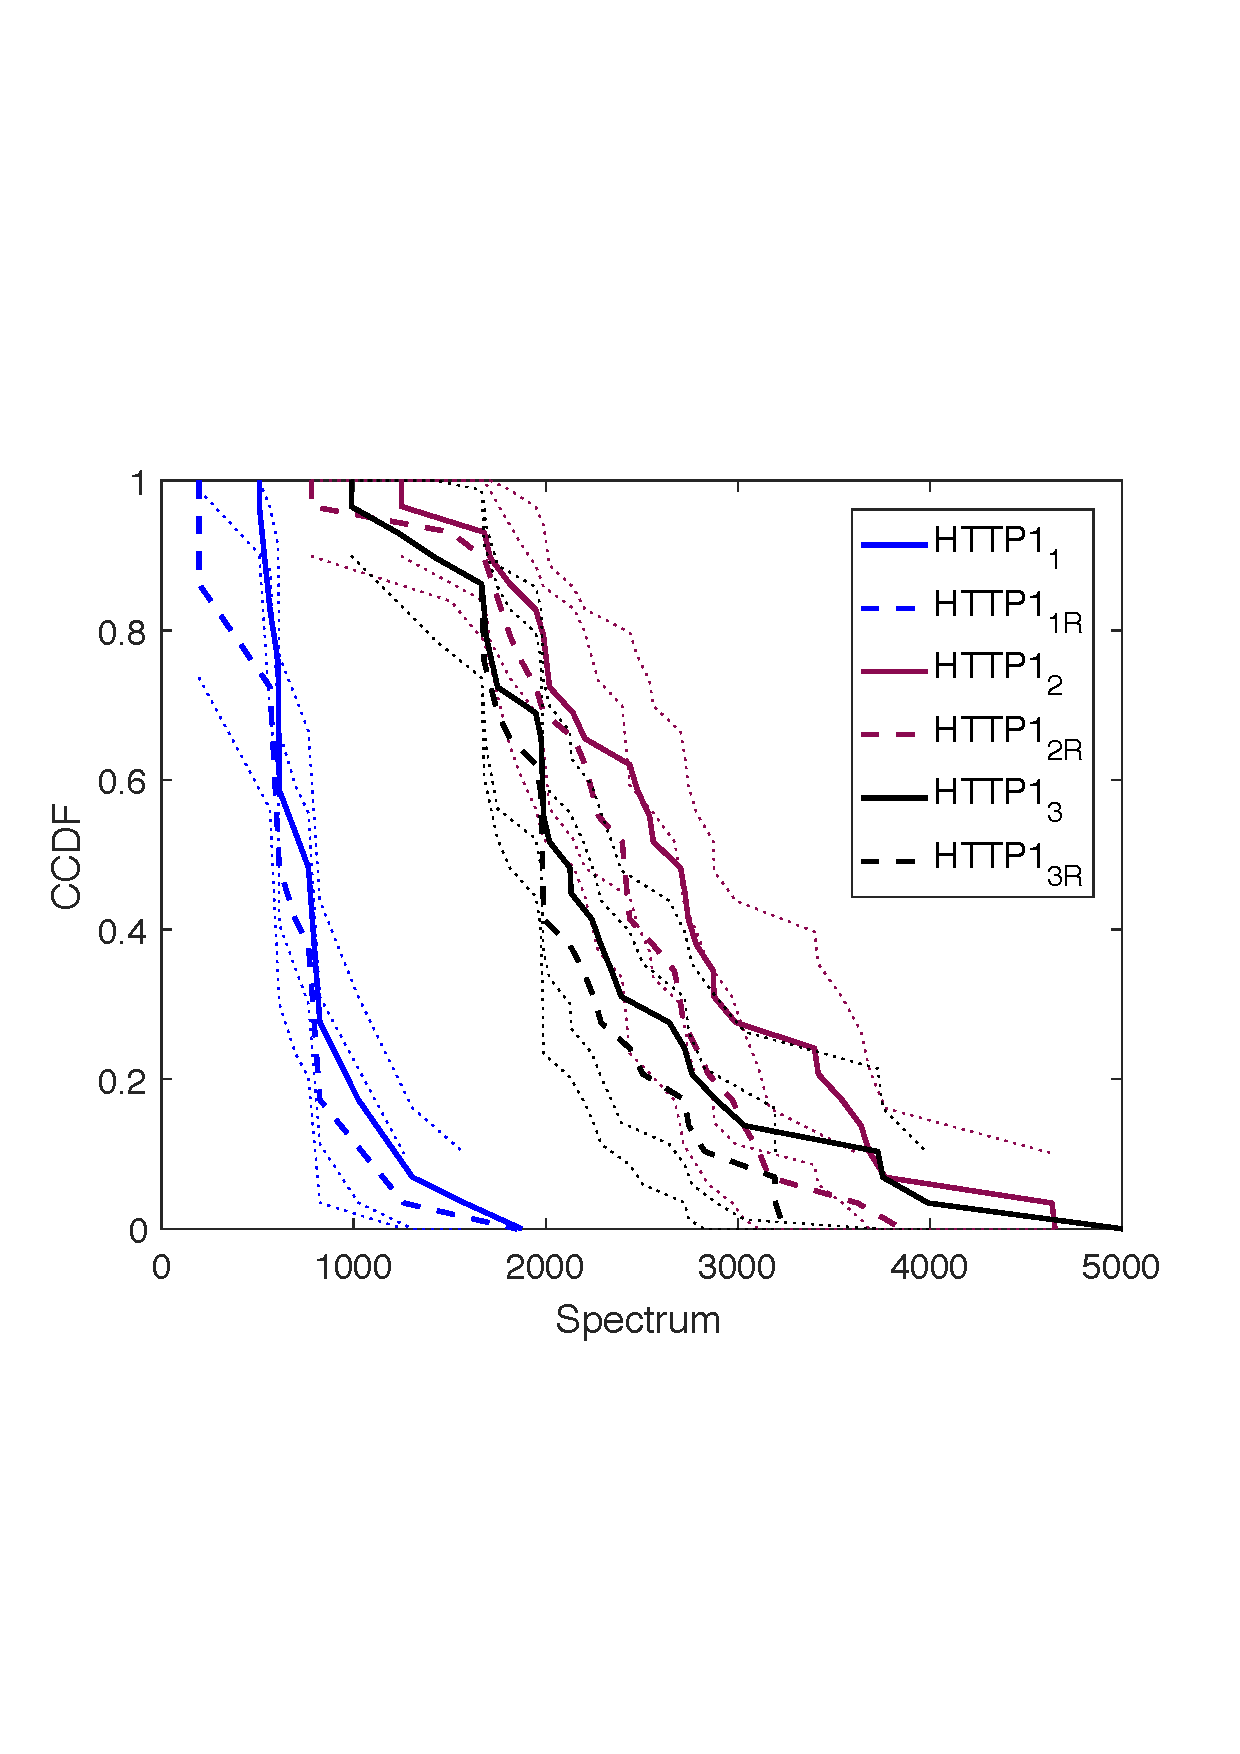
\includegraphics[trim={0 7cm 0 7cm}, scale=0.25]{figures/CDF_magswitch_squad_parallel_http1_nd18.pdf}
    \caption{}
    \label{fig:phttp1magsw}
  \end{subfigure}
 \centering
  \caption{Parallel Client Measurements - Three HTTP1.1 Clients. Client 1 experiences a significantly higher QoE. Since HTTP1.1 does not support multiplexing, the clients request segments of heterogenous quality bitrates sequentially causing the QoE performance to be significantly different.}
  \label{fig:phttp1}
\end {figure*}
\begin{figure*}[t!]
\centering
\begin{subfigure}[t]{0.33\textwidth}
   \captionsetup{justification=centering,margin=4.5cm}
    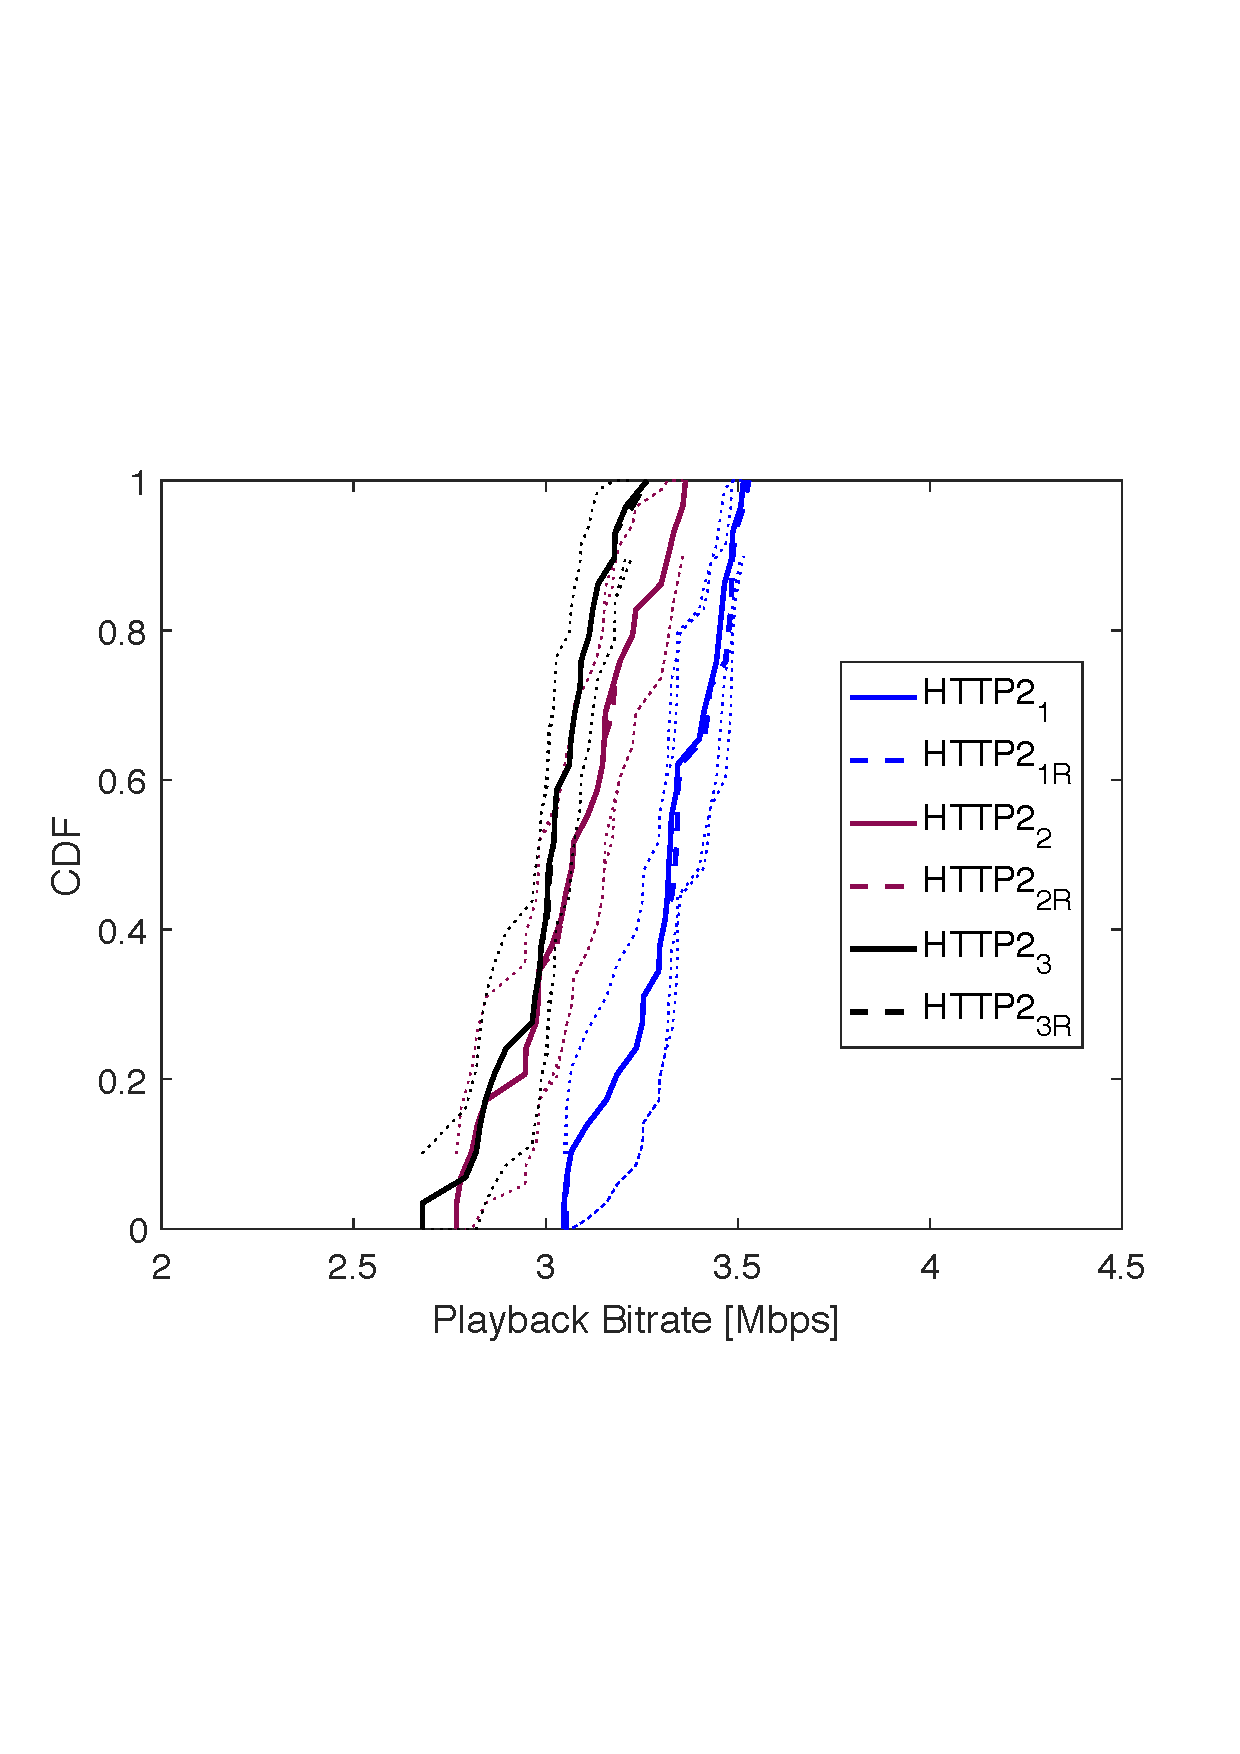
\includegraphics[trim={0 7cm 0 7cm}, scale=0.25]{figures/CDF_bitrat_squad_parallel_http2_nd18.pdf}
     \caption{}
    \label{fig:phttp2bitrate}
  \end{subfigure}
  \begin{subfigure}[t]{0.33\textwidth}
  \captionsetup{justification=raggedright,singlelinecheck=false,margin=2.5cm}
    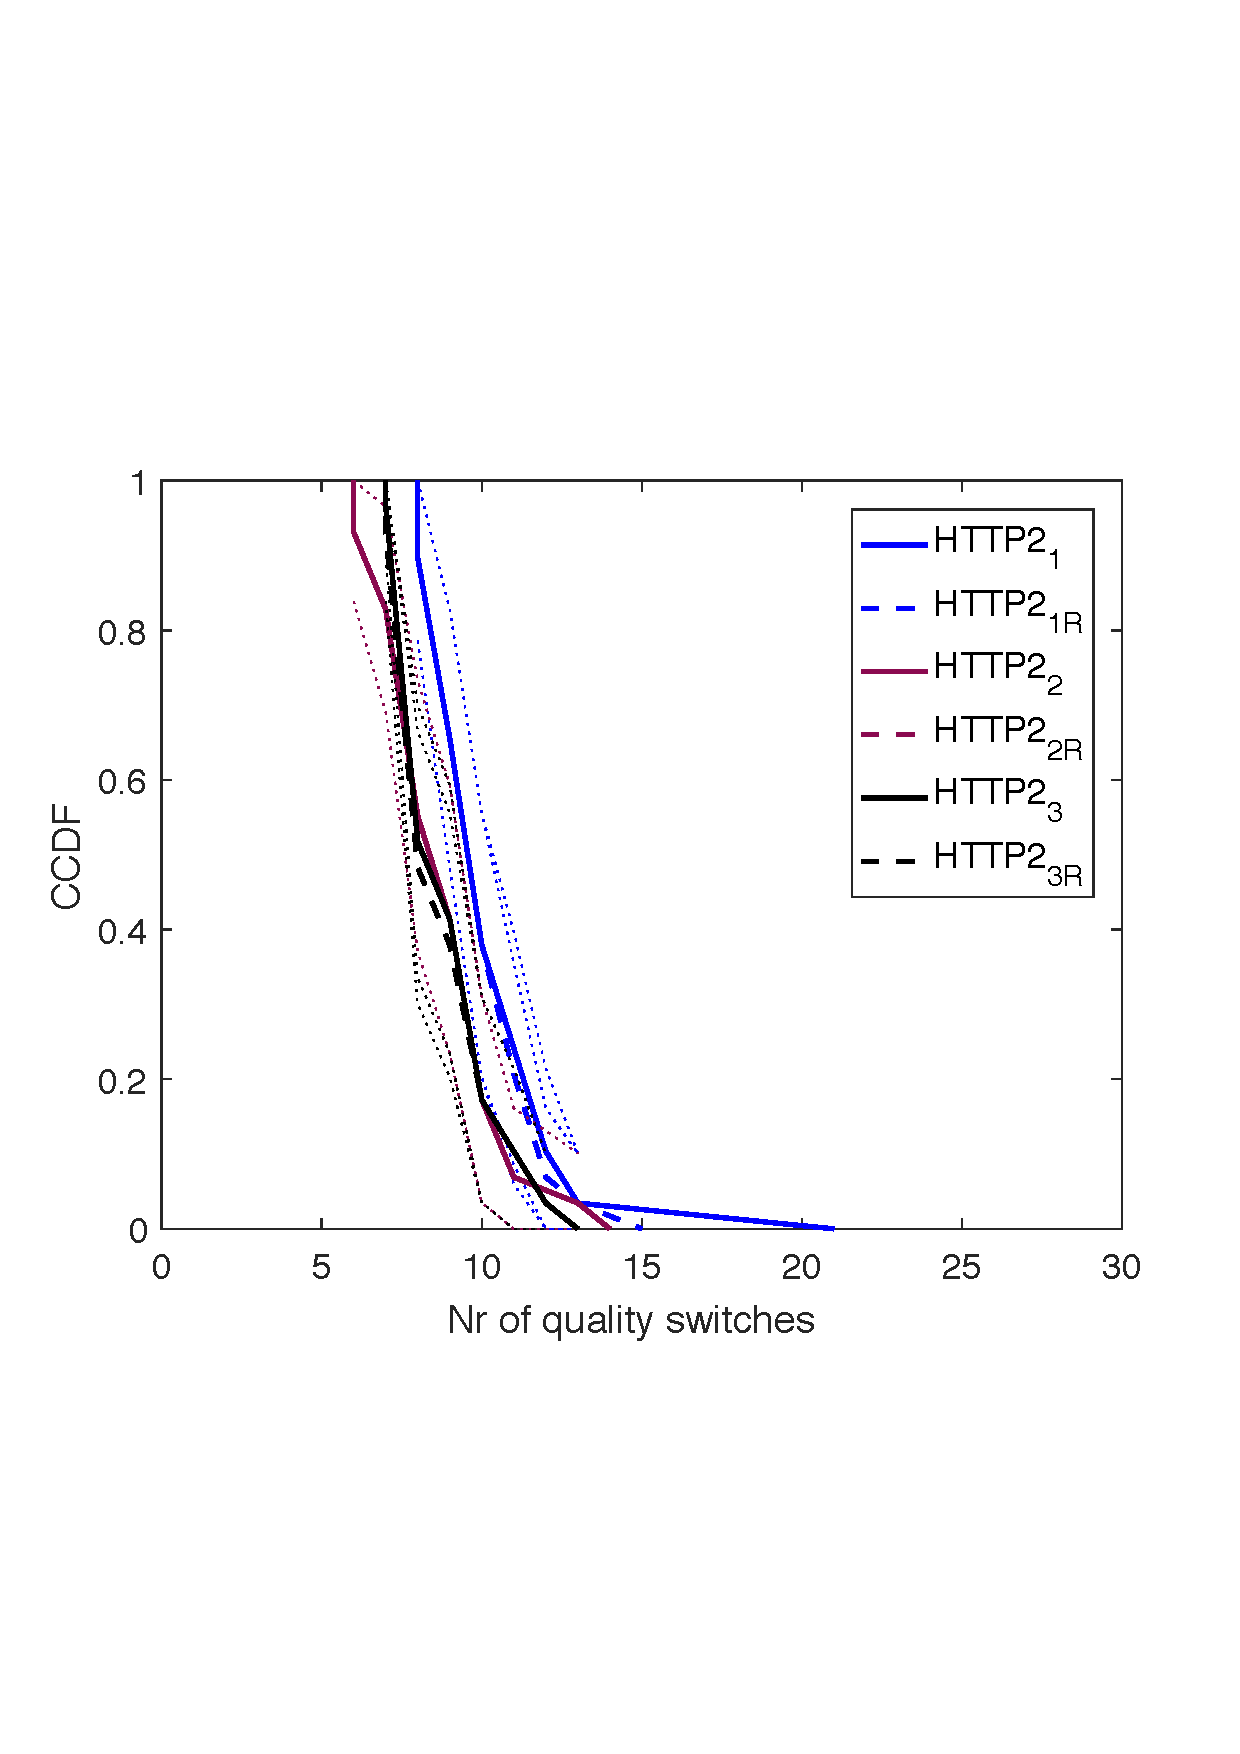
\includegraphics[trim={0 7cm 0 7cm}, scale=0.25]{figures/CDF_cntswitch_squad_parallel_http2_nd18.pdf}
    \caption{}
    \label{fig:phttp2cntsw}
  \end{subfigure}
  \begin{subfigure}[t]{0.33\textwidth}
  \captionsetup{justification=centering,margin=1.5cm}
    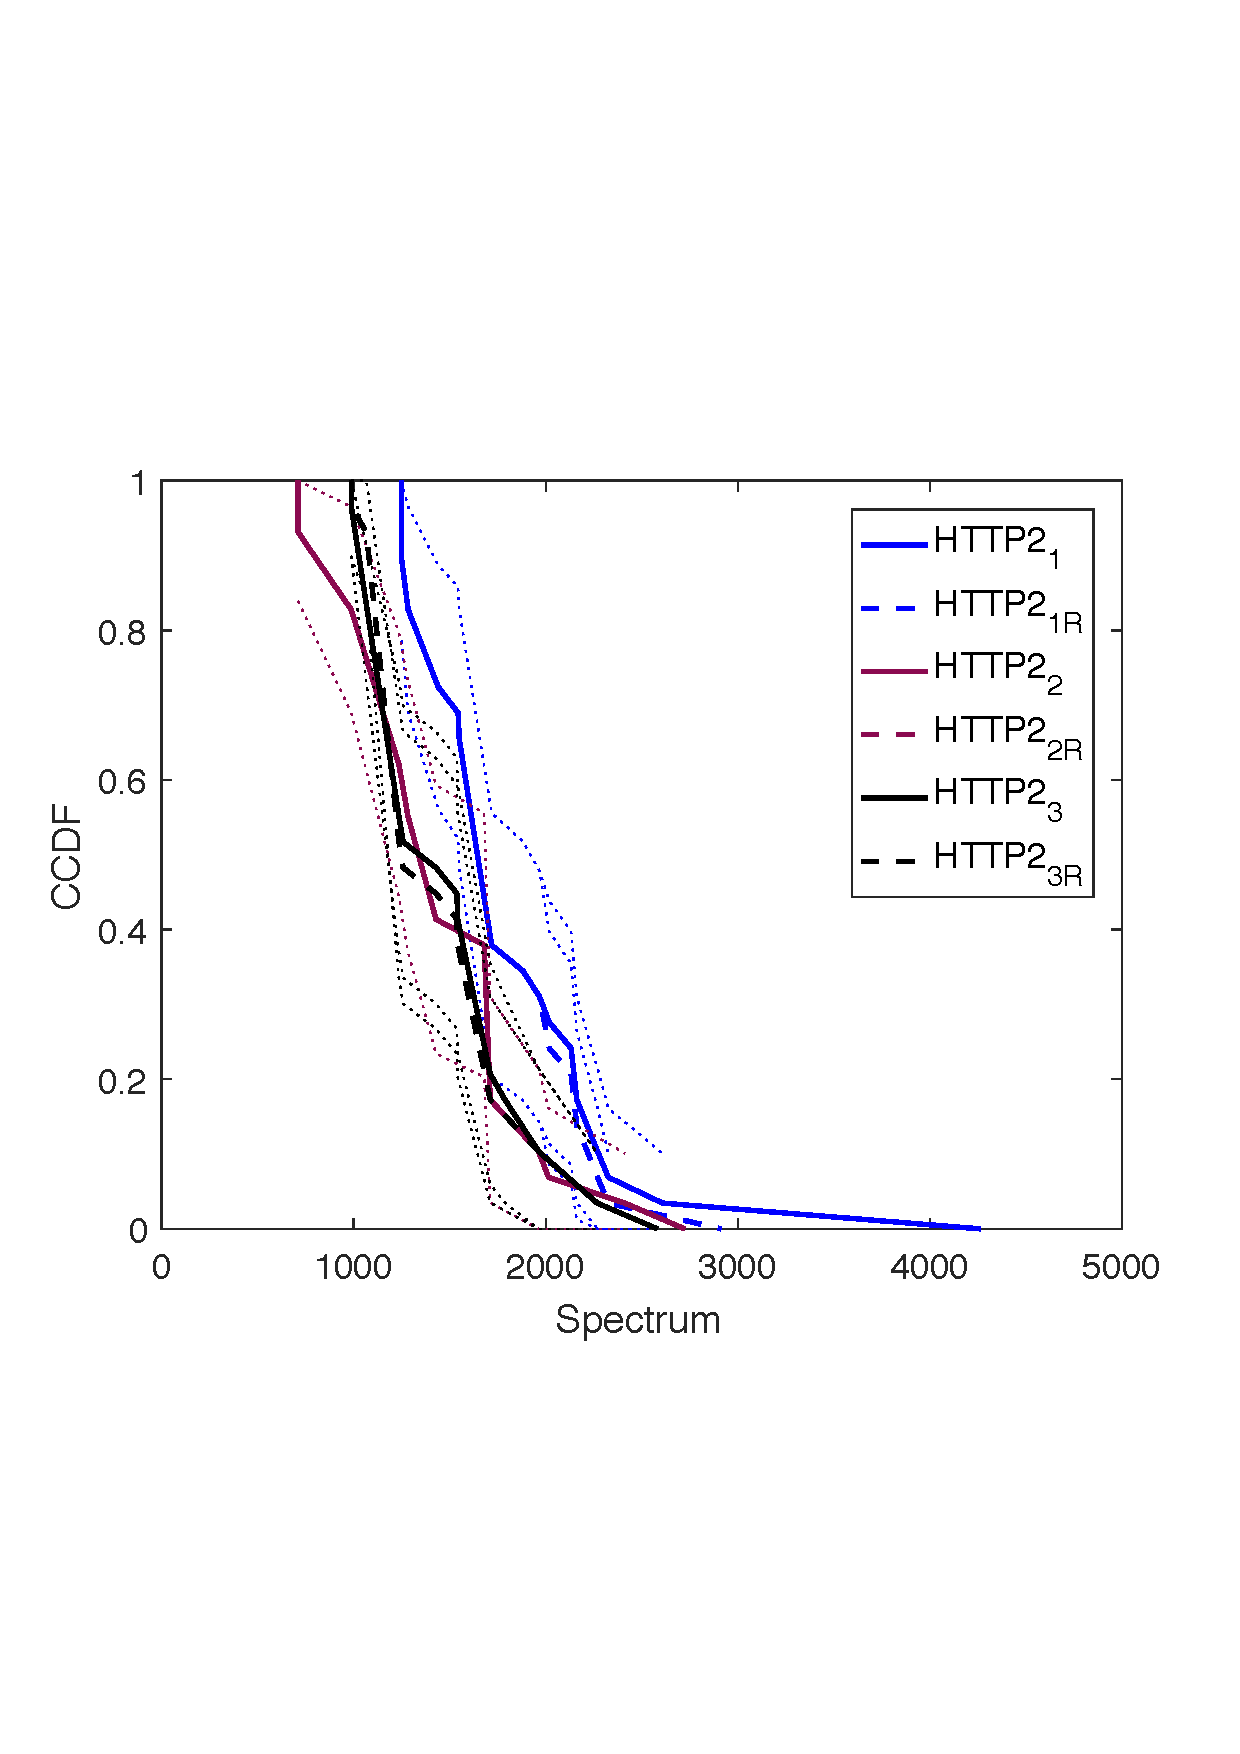
\includegraphics[trim={0 7cm 0 7cm}, scale=0.25]{figures/CDF_magswitch_squad_parallel_http2_nd18.pdf}
    \caption{}
    \label{fig:phttp2magsw}
  \end{subfigure}
 \centering
  \caption{Parallel Client Measurements - Three HTTP2 Clients. All three clients experience comparable QoE and HTTP/HTTP/2 exhibits fairness compared to QUIC. However, the average bitrate is low since HTTP/2 supports multiplexing but continues to be limited by TCP parameters, which leads to conservative behavior.}
  \label{fig:phttp2}
\end {figure*}
\begin{figure*}[t!]
\centering
\begin{subfigure}[t]{0.33\textwidth}
   \captionsetup{justification=centering,margin=4.5cm}
    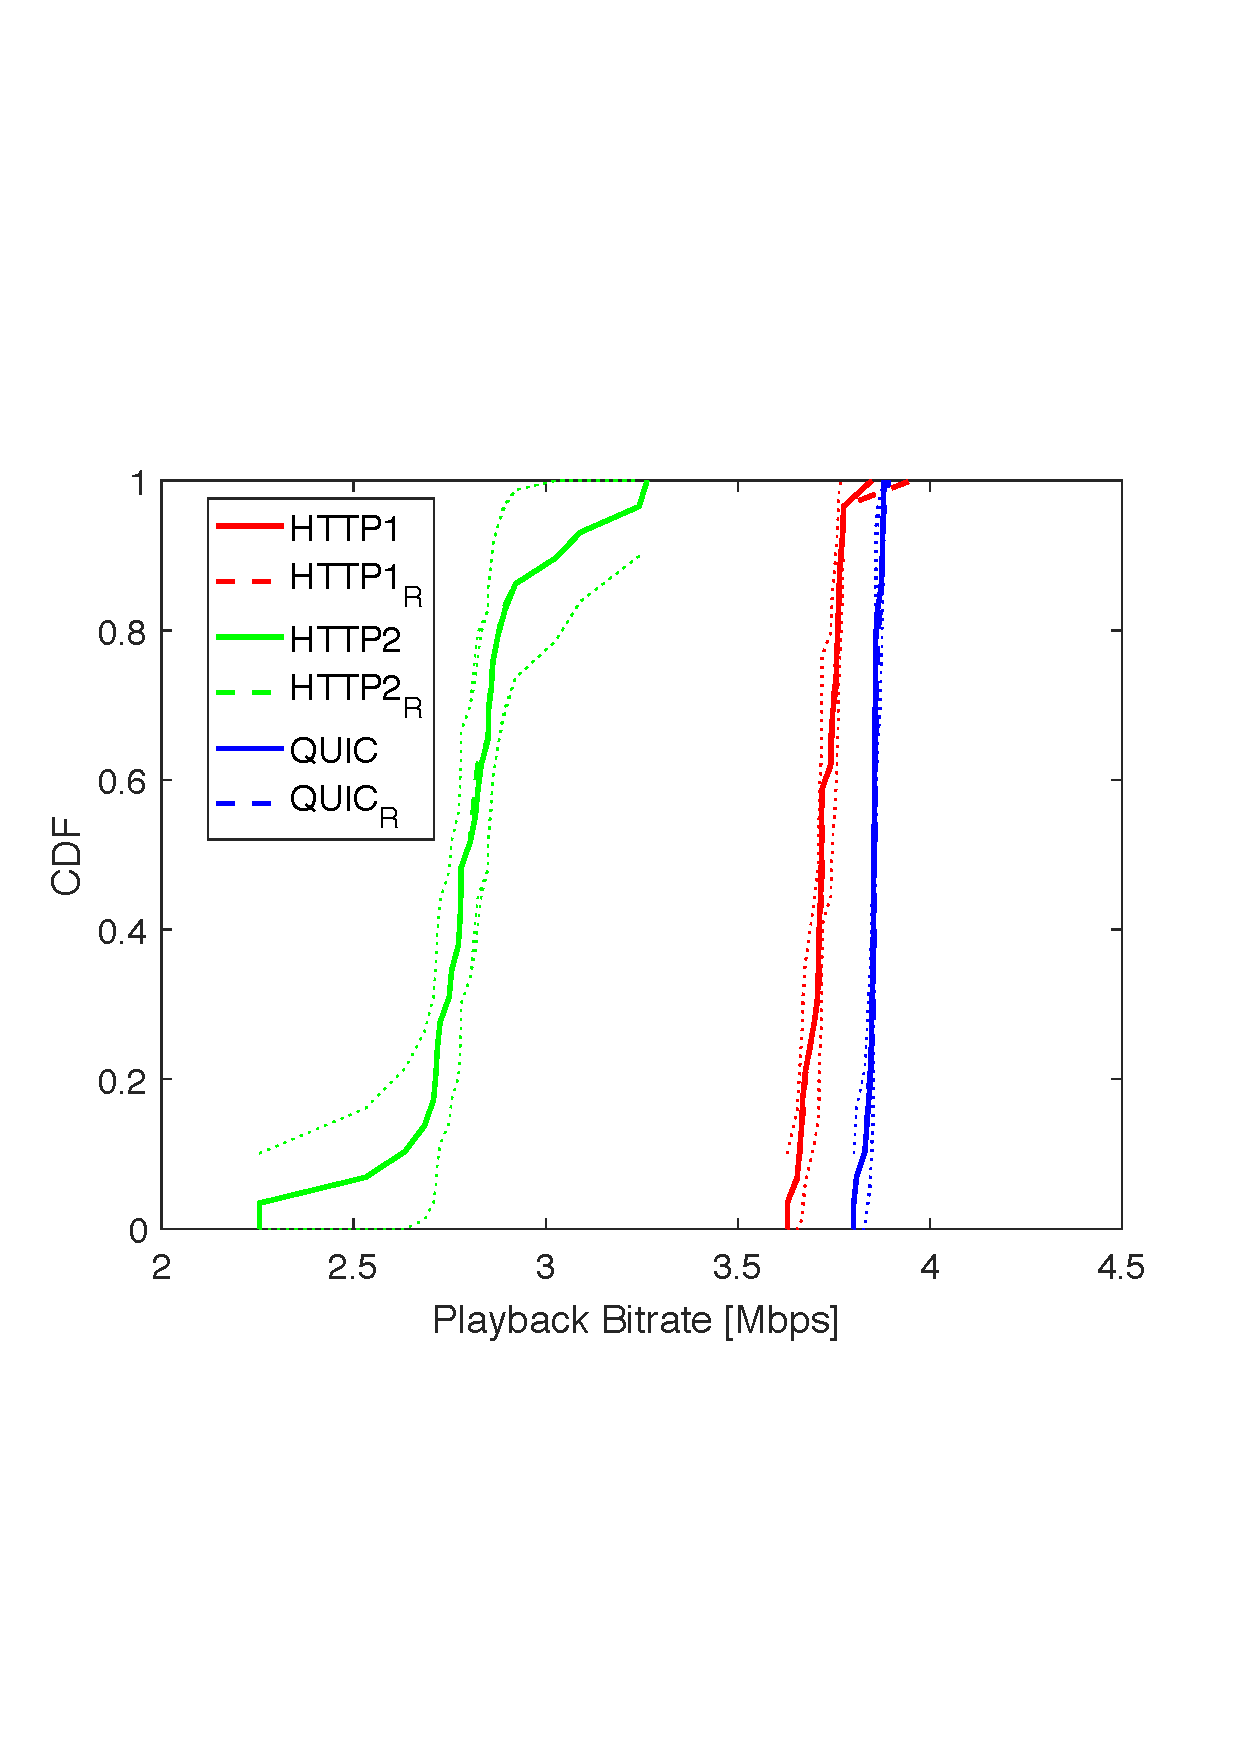
\includegraphics[trim={0 7cm 0 7cm}, scale=0.25]{figures/CDF_bitrat_squad_mixed_clients_nd18.pdf}
     \caption{}
    \label{fig:pmixedbitrate}
  \end{subfigure}
  \begin{subfigure}[t]{0.33\textwidth}
  \captionsetup{justification=raggedright,singlelinecheck=false,margin=2.5cm}
    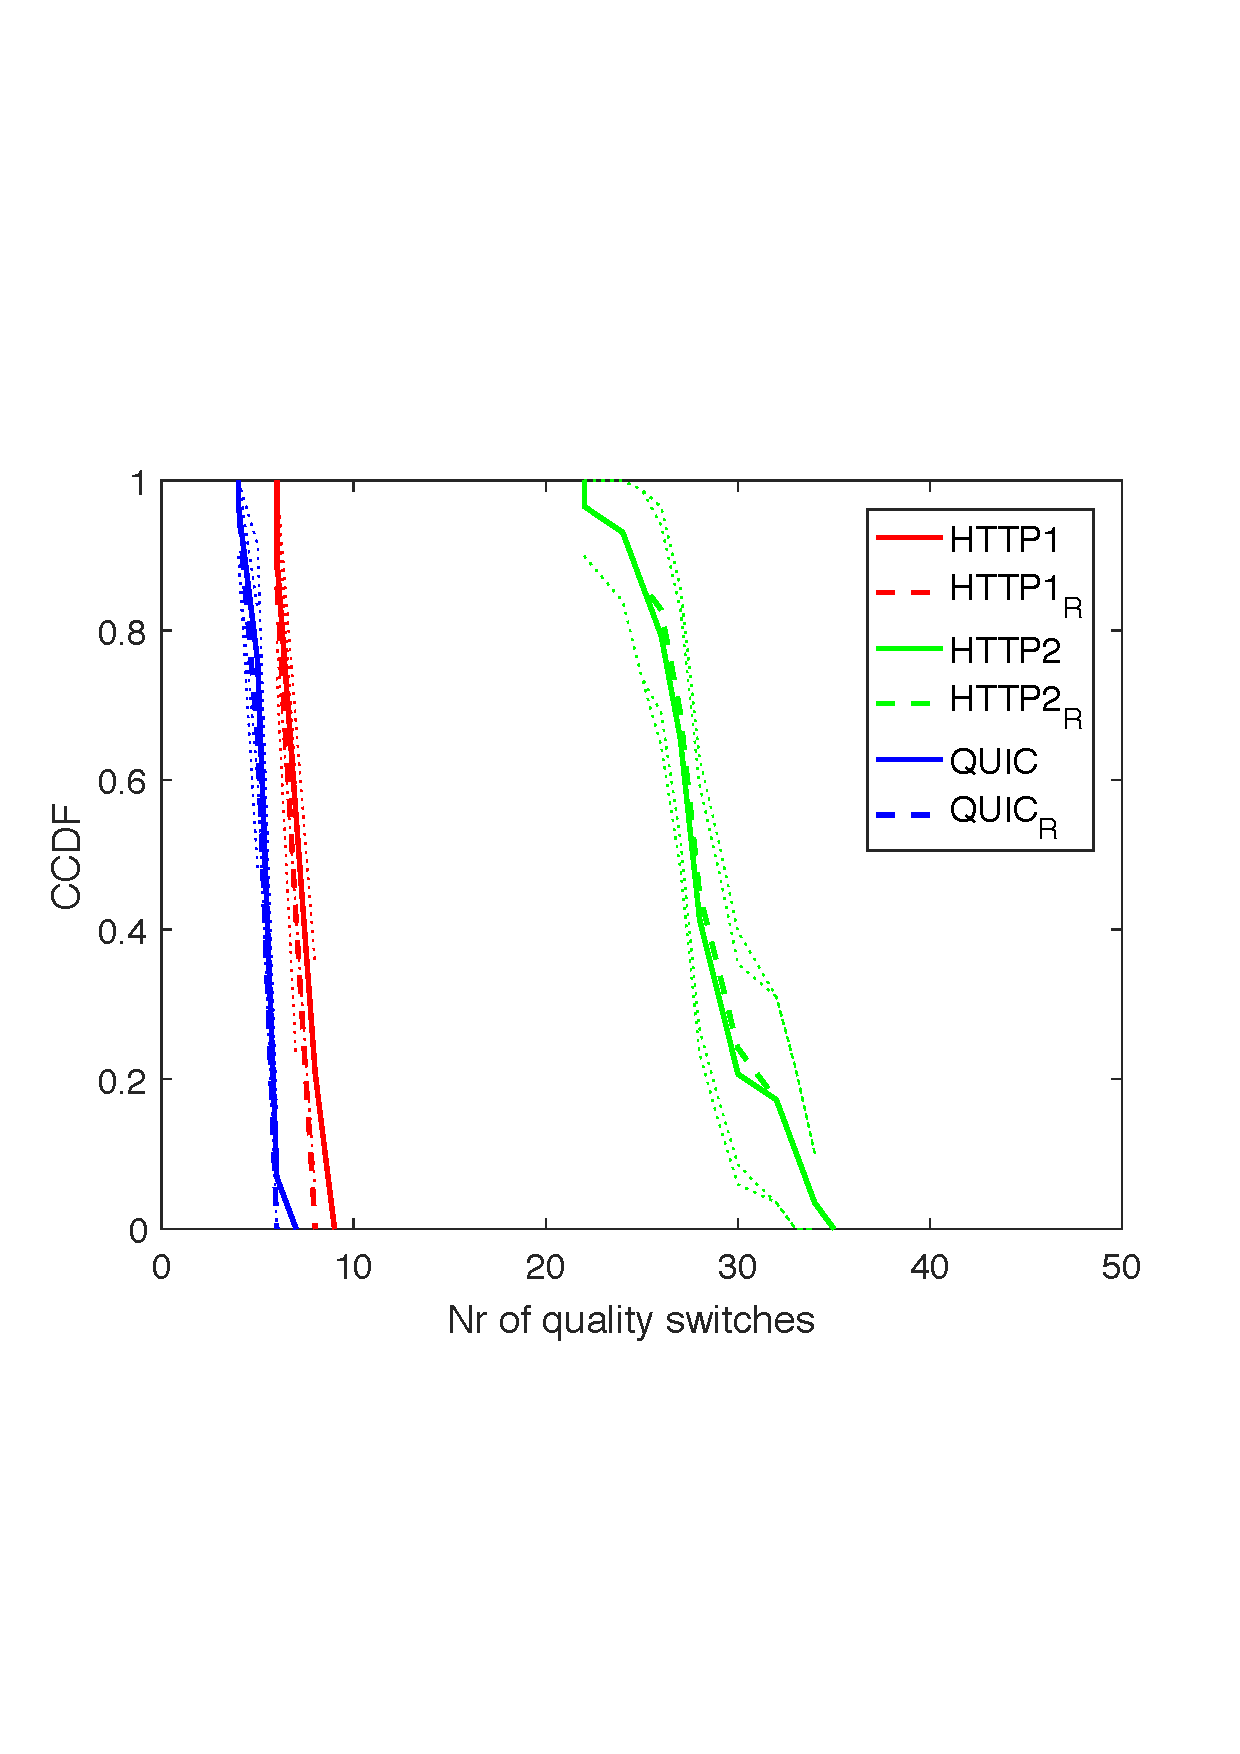
\includegraphics[trim={0 7cm 0 7cm}, scale=0.25]{figures/CDF_cntswitch_squad_mixed_clients_nd18.pdf}
    \caption{}
    \label{fig:pmixedcntsw}
  \end{subfigure}
  \begin{subfigure}[t]{0.33\textwidth}
  \captionsetup{justification=centering,margin=1.5cm}
    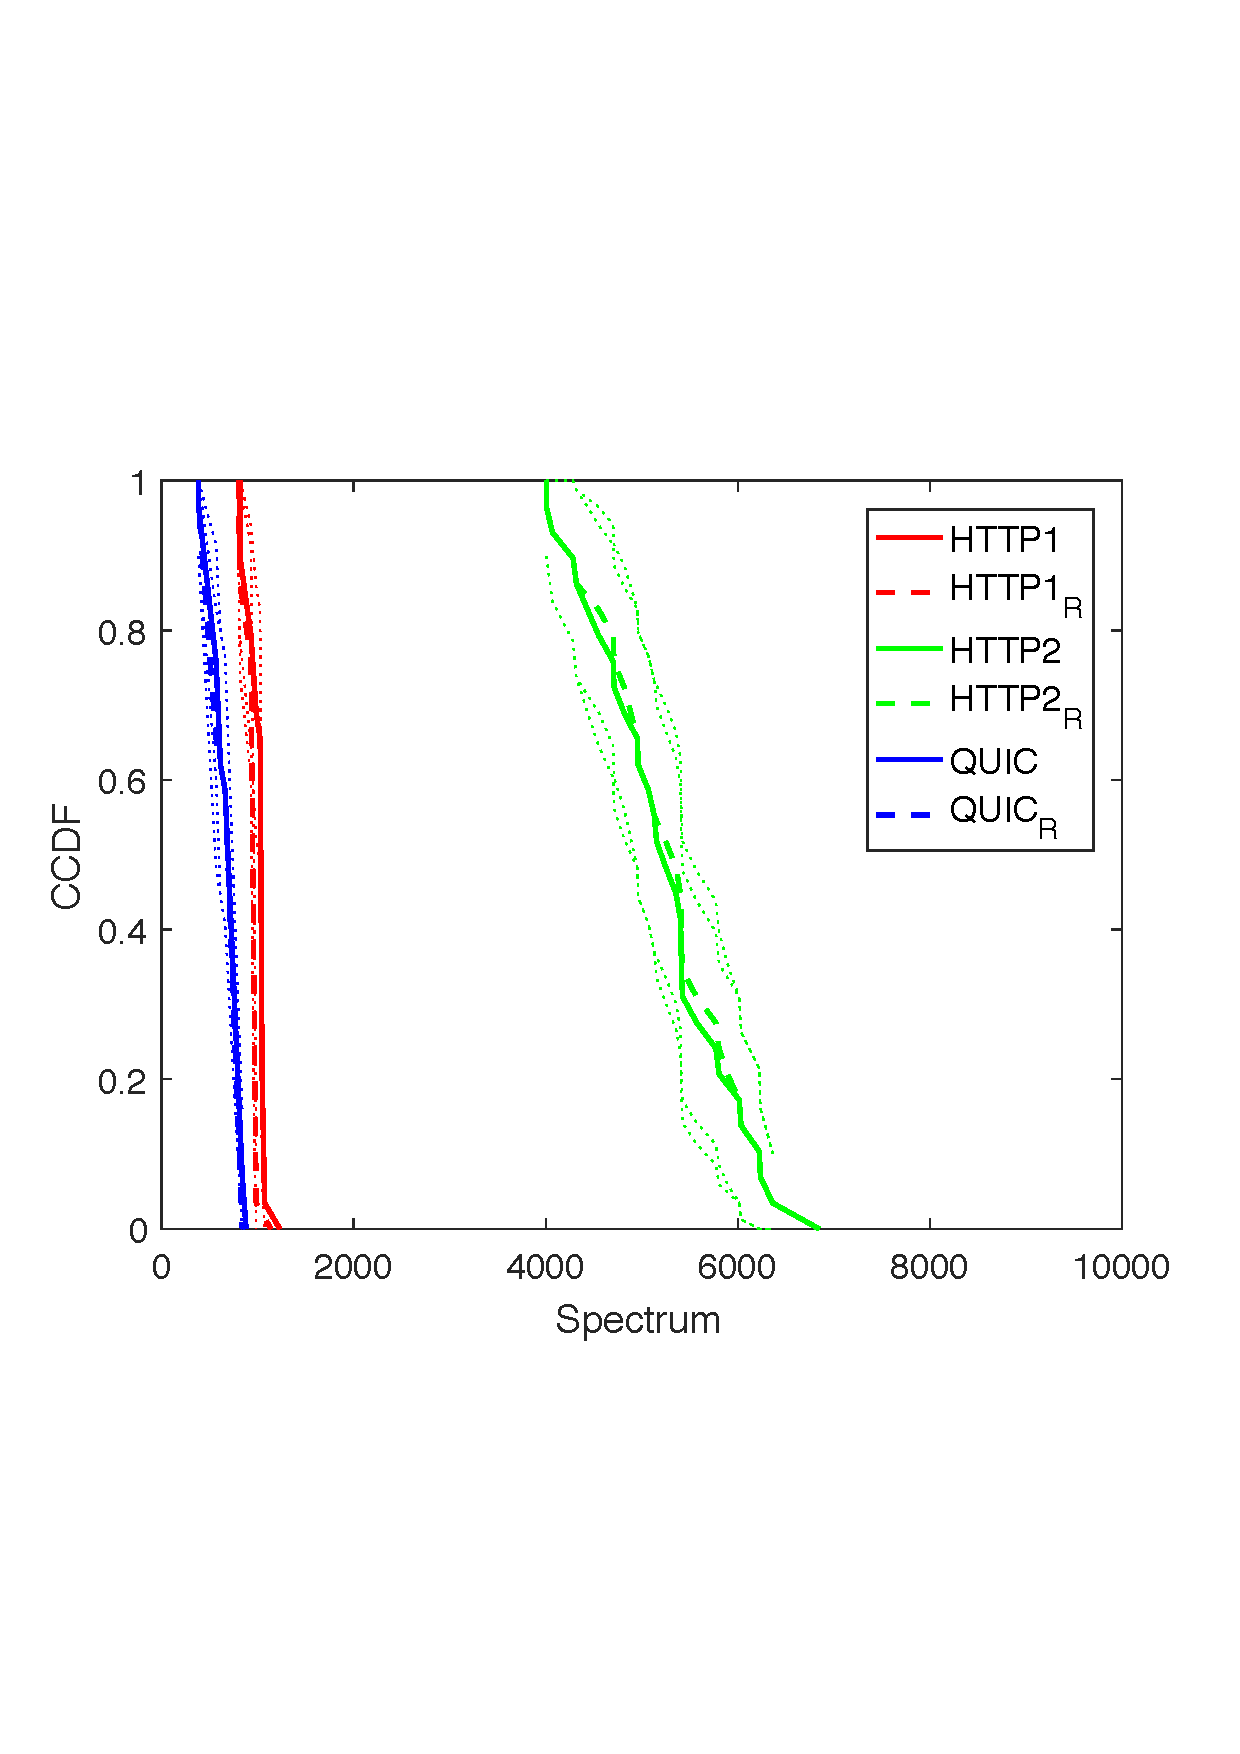
\includegraphics[trim={0 7cm 0 7cm}, scale=0.25]{figures/CDF_magswitch_squad_mixed_clients_nd18.pdf}
    \caption{}
    \label{fig:pmixedmagsw}
  \end{subfigure}
    \begin{subfigure}[t]{0.33\textwidth}
  \captionsetup{justification=raggedright,singlelinecheck=false,margin=2.5cm}
    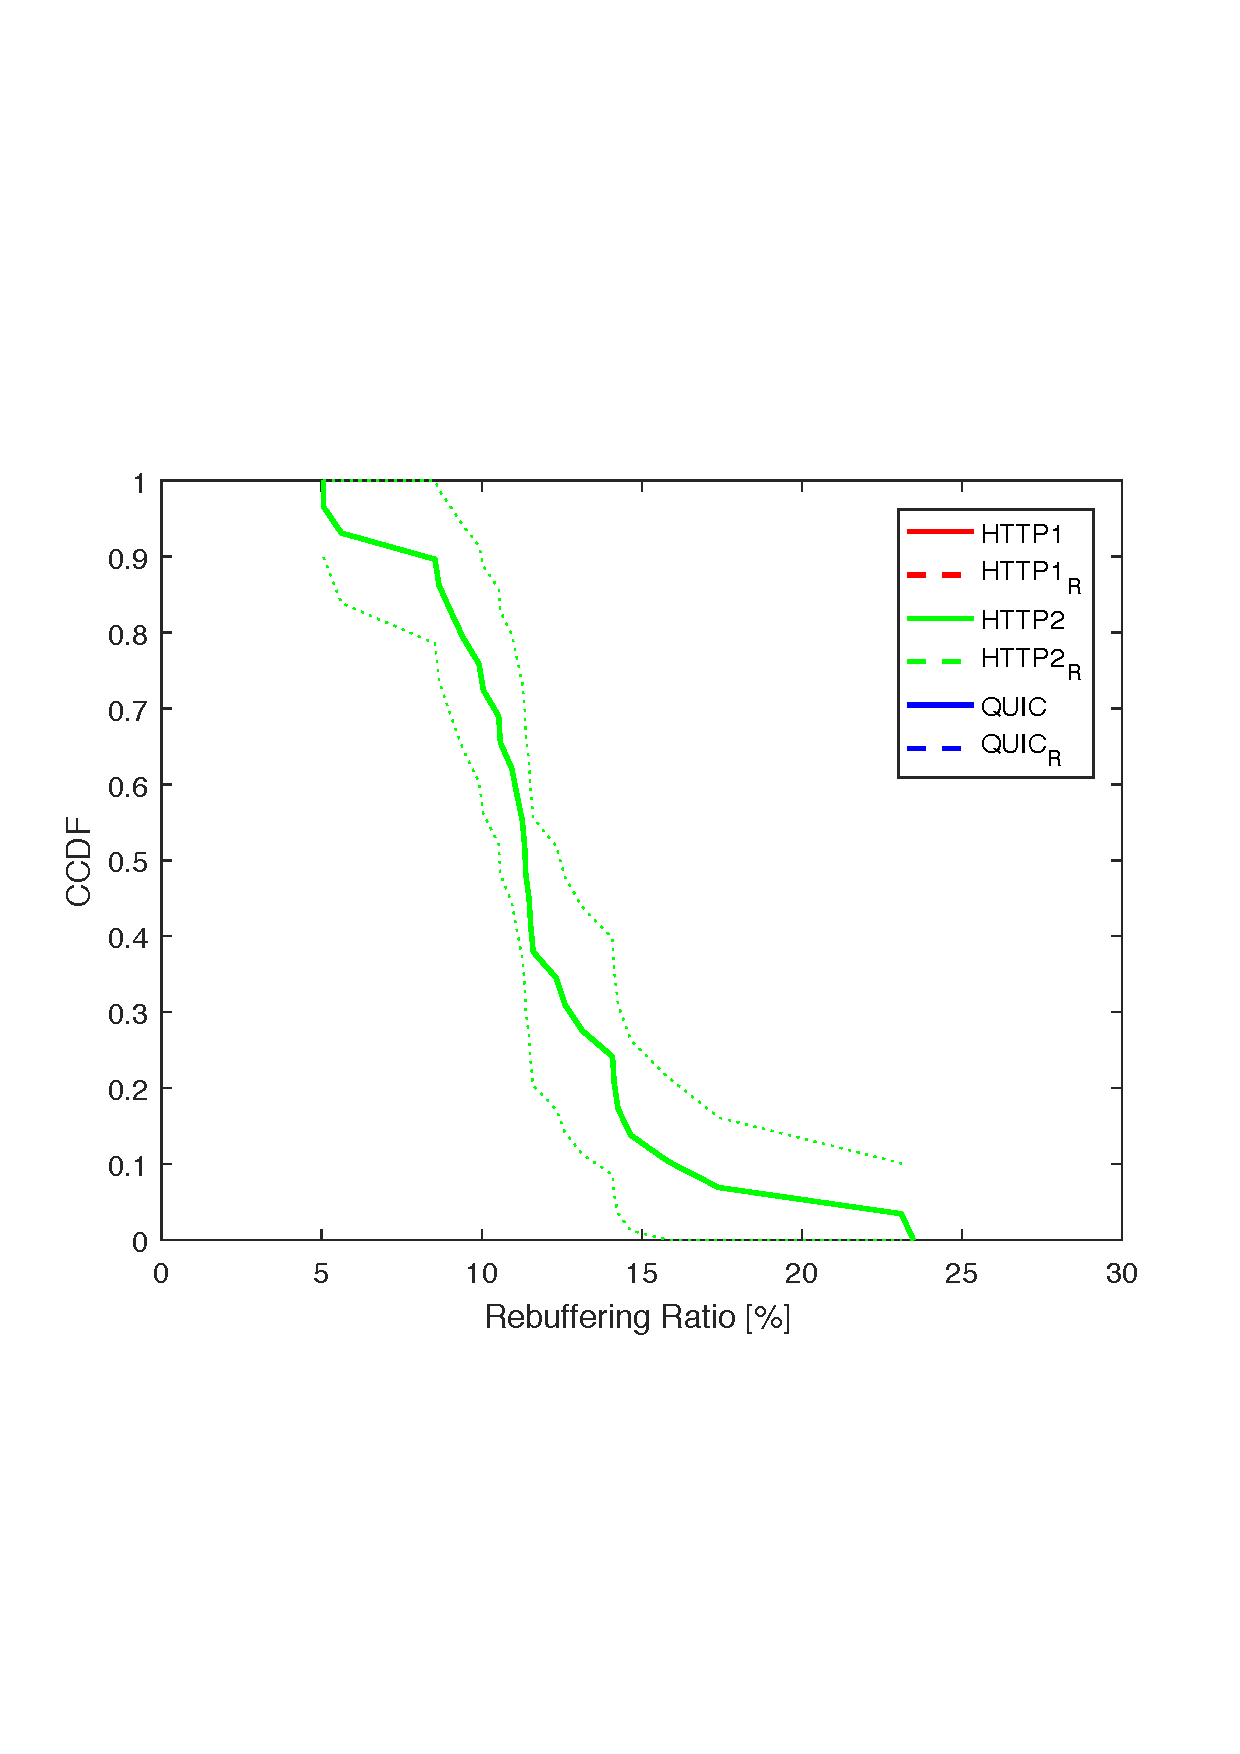
\includegraphics[trim={0 7cm 0 7cm}, scale=0.25]{figures/CDF_rebuffer_squad_mixed_clients_nd18.pdf}
    \caption{}
    \label{fig:pmixedrebuf}
  \end{subfigure}
 \centering
  \caption{Parallel Client Measurements - One HTTP1.1, one HTTP/2 and one QUIC Client. HTTP/2 experiences the worst QoE of all while QUIC clients perform comparatively better than HTTP1.1.}
  \label{fig:pmixed}
\end {figure*}
\fi
\begin{table}[h]
\centering
 \begin{tabular}{ | l | c | c | r | }
    \hline
      & \textit{Client1} & \textit{Client2} & \textit{Client3}\\ \hline \hline
     Average \%Retransmissions & 0.8$\pm$1.3  &1.7$\pm1.3$  &1.0$\pm$0.9  \\
    \hline
  \end{tabular}
  \caption{ABR Segment Retransmissions for three parallel QUIC clients}
           \vspace{-30pt}
    \label{tab:retx_parallel_quic}
    \centering
\end{table}
%with the default Explicit Congestion Notification (ECN) setting, i.e, we enable ECN when requested by incoming connections but do not request ECN on outgoing connections \MZ{[Is %the information about ECN essential for our work or can we take it out?]}. 
\subsection{Internet}
\begin{figure*}[t!]
\centering
\begin{subfigure}[t]{0.33\textwidth}
   \captionsetup{justification=centering,margin=4.5cm}
    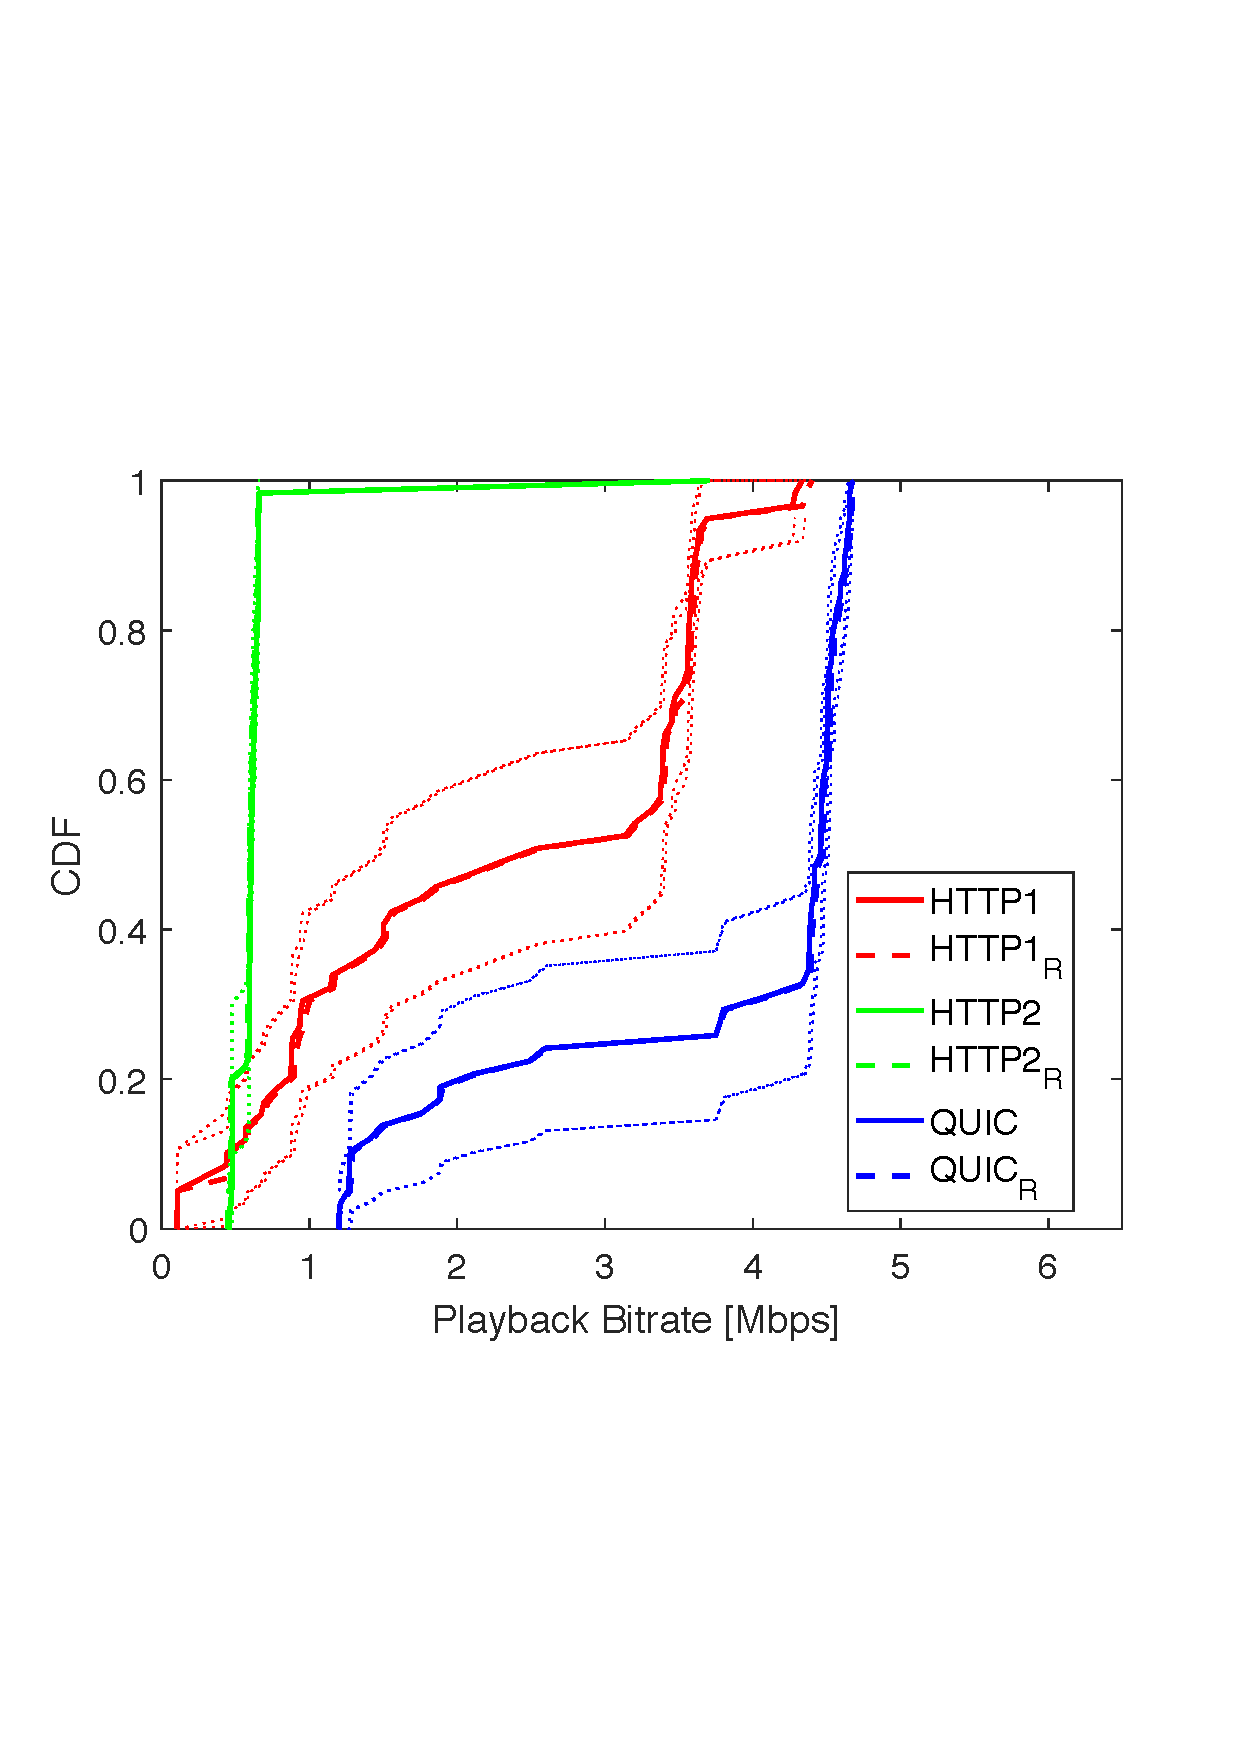
\includegraphics[trim={0 7cm 0 7cm}, scale=0.25]{figures/CDF_bitrat_squad_ec2Mumbai_nd18.pdf}
     \caption{}
    \label{fig:ec2Mumbaibitrate}
  \end{subfigure}
  \begin{subfigure}[t]{0.33\textwidth}
  \captionsetup{justification=raggedright,singlelinecheck=false,margin=2.5cm}
    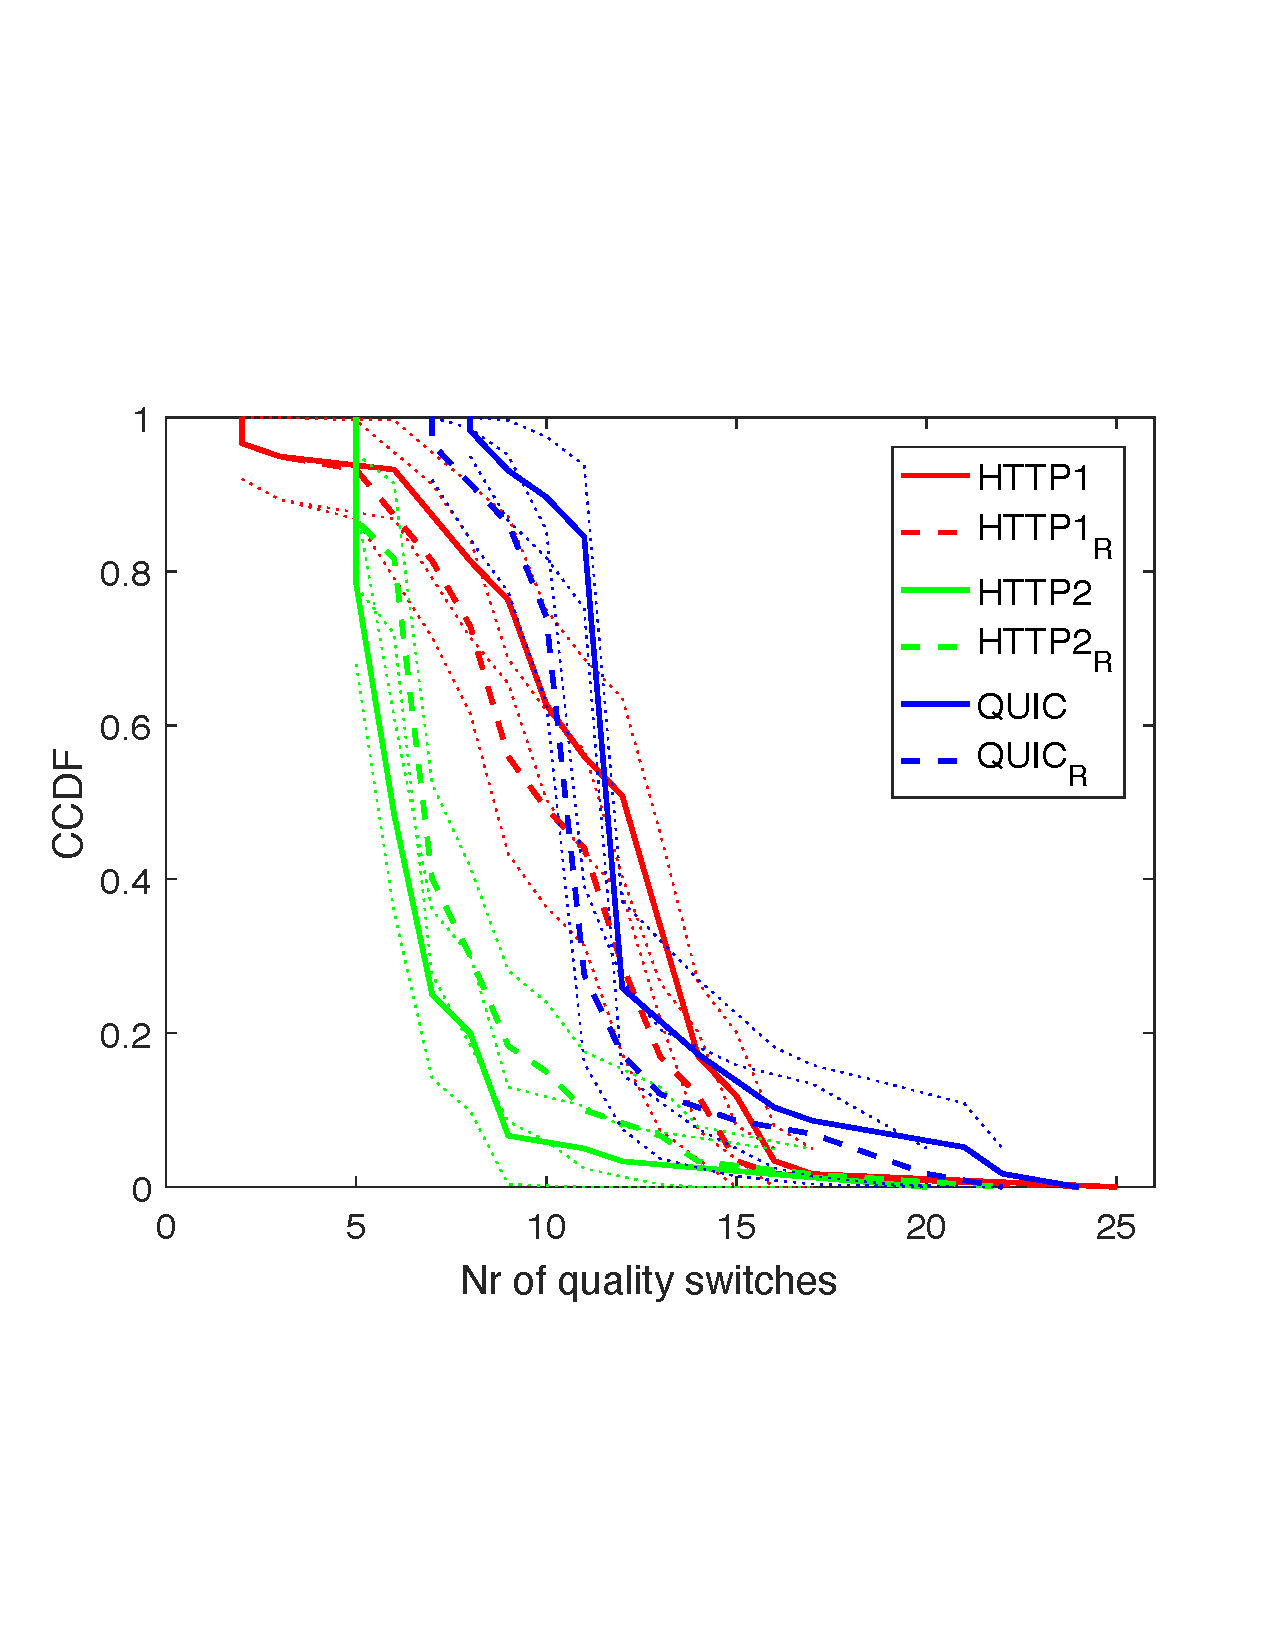
\includegraphics[trim={0 6cm 0 7cm}, scale=0.25]{figures/CDF_cntswitch_squad_ec2Mumbai_nd18.pdf}
    \caption{}
    \label{fig:ec2Mumbaicntswitch}
  \end{subfigure}
  \begin{subfigure}[t]{0.33\textwidth}
  \captionsetup{justification=centering,margin=1.5cm}
    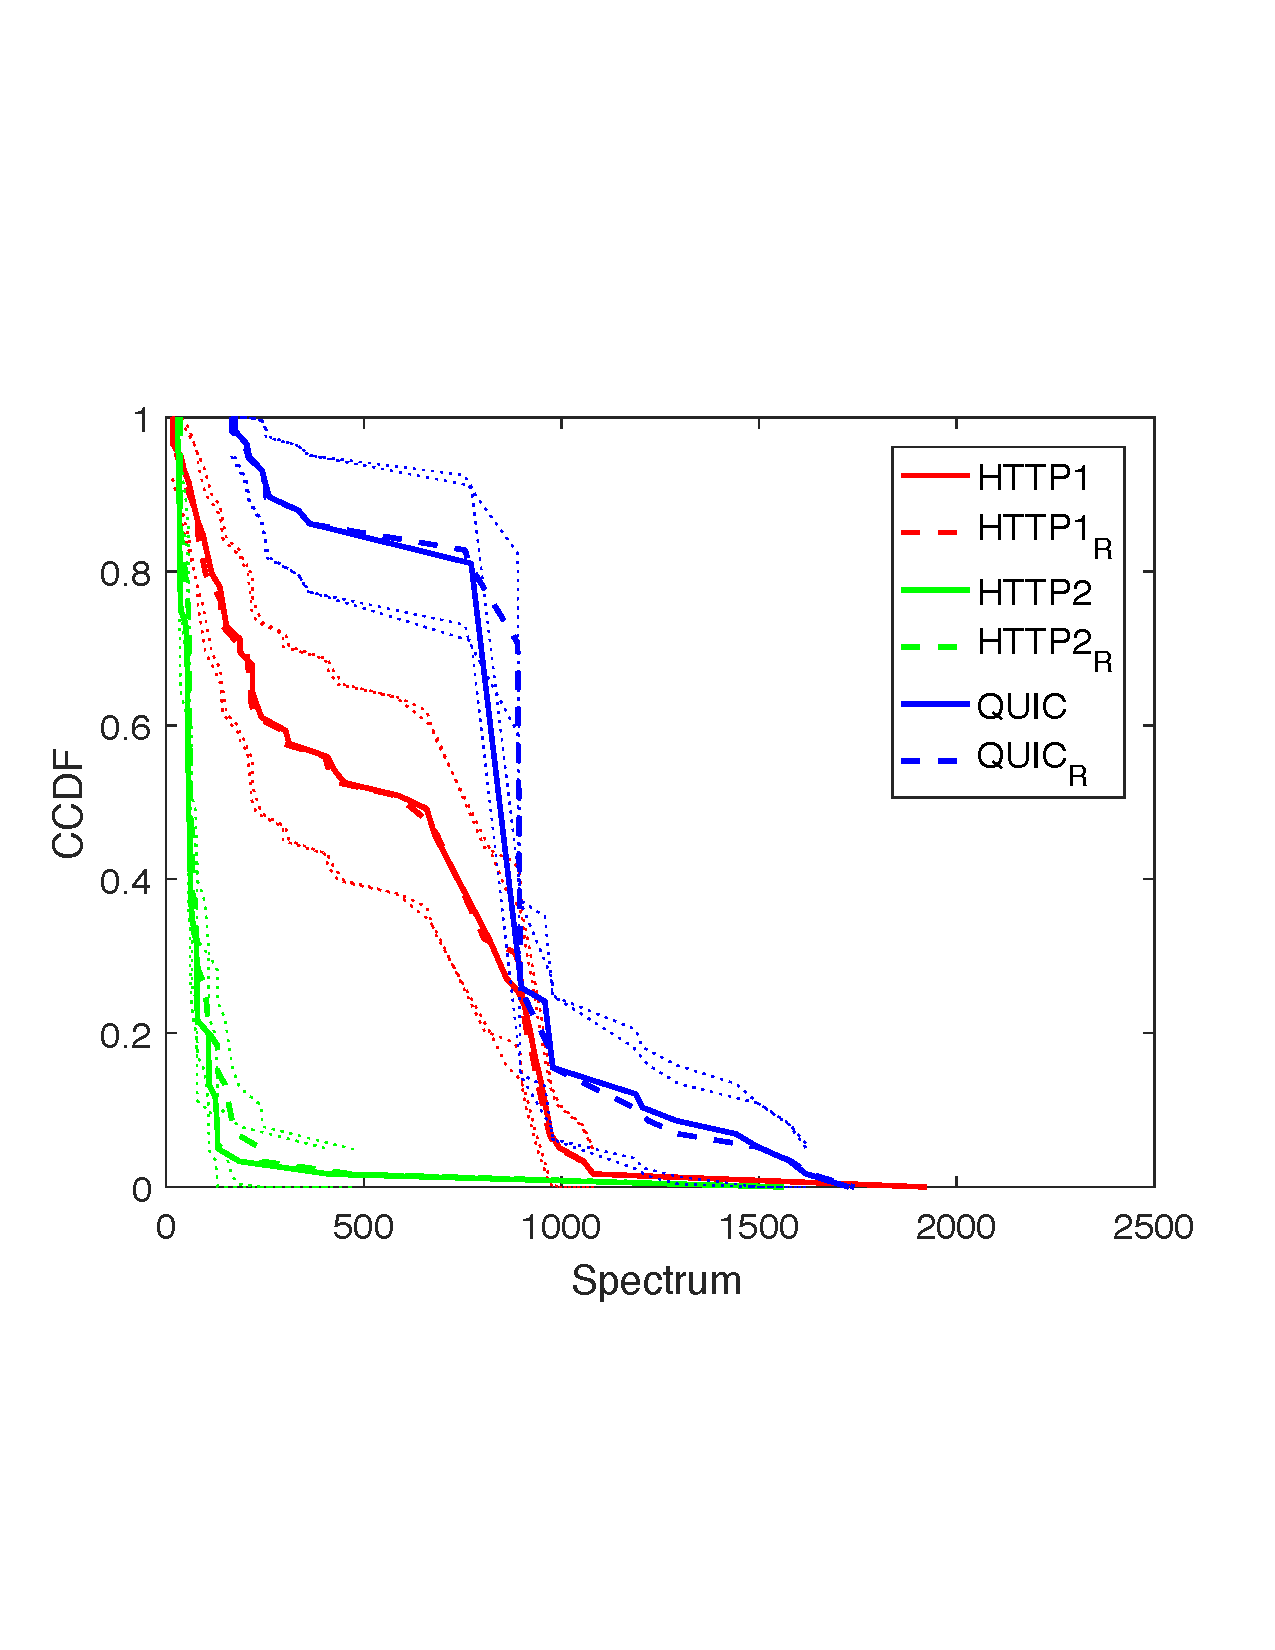
\includegraphics[trim={0 6cm 0 7cm}, scale=0.25]{figures/CDF_magswitch_squad_ec2Mumbai_nd18.pdf}
    \caption{}
    \label{fig:ec2Mumbaimagswitch}
  \end{subfigure}
 \centering
   \vspace{-15pt}
  \caption{Internet Measurements - ABR streaming is performed over inter-continental links with the server at Amazon EC2 in India and the client on the US East Coast. QUIC far outperforms HTTP/1.1 and HTTP/2 in terms of QoE, i.e., provides significant improvement in Average Quality Bitrate while providing comparable reduction in the number of quality switches.}
  \label{fig:ec2Mumbai}
  \vspace{-10pt}
\end {figure*}
For the Internet measurements, we use Amazon EC2 virtual machines in Mumbai, India and Oregon, USA as servers and a client in the UMass Amherst campus network to perform inter-continental and intra-continental measurements, respectively. Here, we repeat each experiment 60 times to account for increased network variations in an uncontrolled environment. Since the bottleneck bandwidth during off-peak hours can be high, we use a different video dataset with higher qualities, \texttt{RedBull} \cite{lederer2012dynamic}, and modify the MPD to contain the following bitrates $\{${0.10, 0.15, 0.20, 0.25, 0.30, 0.40, 0.50, 0.70, 
0.90, 1.20, 1.50, 2.00, 2.50, 3.00, 4.00, 5.00, 6.00}$\}$Mbps for a video duration of 300s and a segment duration of 2s.
Figure \ref{fig:ec2Mumbai} presents results for measurements "in the wild" over inter-continental links from an EC2 web server located in India. The average quality bitrate (in Fig. \ref{fig:ec2Mumbaibitrate}) is significantly higher for QUIC than HTTP/2 and HTTP/1.1. Fig. \ref{fig:ec2Mumbaicntswitch} shows that $\#QS$ is also reduced with the use of QUIC and HTTP/1.1 retransmissions indicating an overall high QoE. Table \ref{tab:qoe_abr_internet} shows QoE metrics for similar measurements conducted with the server located at EC2 in Oregon. Here, it is worth mentioning that all QoE metrics are comparable for HTTP/1.1 and QUIC where QUIC is marginally better than HTTP/1.1, but are significantly improved over HTTP/2 (for example, the average bitrate $AQB$ is less than half of that obtained with HTTP/1.1 and QUIC). Since Internet traffic is predominantly comprised of TCP flows, these results further reinforce the observations made in Sect. \ref{subsubsec:hol} for high delay, high loss paths with competing TCP traffic. Our results show that the use of QUIC results in better QoE in the case of inter-continental as well as intra-continental links, while the advantage compared to HTTP/1.1 is more significant in case of the former.

\begin{comment}
\begin{table*}[h]
\centering
 \begin{tabular}{ | l | c | c | c | c | c | c | r | }
    \hline
      & $AQB$ (Mbps) &  $AQB_{R}$ (Mbps) & $\#QS$ & $\#QS_{R}$ & $H$ & $H_{R}$ & $RB_{R}$(\%)\\ \hline \hline
     %Single Clients: UDP-W (8M-5M) & 3.90$\pm0.1$ & 3.93$\pm$0.1  & 8.7$\pm$0.9 & 6.1$\pm$1.6 & 1596$\pm$204 & 919$\pm$306 & 0   \\ \hline
     Parallel Clients: HTTP/1.1 &  &  &  &  &  &  &  \\ \hline
     Parallel Clients: HTTP/2 & 3.13$\pm$0.2 & 3.14$\pm$0.2  & 9.58$\pm$2.0 & 9.45$\pm$1.7 & 1616$\pm$499 & 1587$\pm$428 & 0 \\ 
    \hline
  \end{tabular}
  \caption{ABR Quality of Experience: Parallel Clients}
    \label{tab:qoe_abr_ctrl}
    \centering
\end{table*}
\end{comment}
\begin{table*}[h]
\centering
 \begin{tabular}{ | l | c | c | c | c | c | c | r | }
    \hline
      & $AQB$ (Mbps) &  $AQB_{R}$ (Mbps) & $\#QS$ & $\#QS_{R}$ & $H$ & $H_{R}$ & $RB_{R}$(\%)\\ \hline \hline
     Internet: HTTP/1.1 & 5.31$\pm$0.1 & 5.66$\pm$0.1  & 8.48$\pm$1.4 & 3.82$\pm$2.1 & 490$\pm$213 & 242$\pm$312 & 0 \\ \hline
     Internet: HTTP/2 & 2.12$\pm$0.6 & 2.13$\pm$0.6  & 9.09$\pm$2.6 & 6.98$\pm$2.5 & 552$\pm$280 & 447$\pm$255  & 0$\pm$10.8\\ \hline
     Internet: QUIC & 5.31$\pm$1.9 & 5.44$\pm$0.2  & 7.91$\pm$1.8 & 5.81$\pm$1.7 & 445$\pm$299 & 351$\pm$273  & 0\\
    \hline
  \end{tabular}
  \caption{ABR Quality of Experience over the Internet: Amazon EC2 Oregon - US East Coast}
  \vspace{-20pt}
    \label{tab:qoe_abr_internet}
    \centering
\end{table*}